\documentclass[]{article}
\usepackage{hyperref}

% Using the caption package allows us to support captions that contain "itemize" environments.
% The font=small option makes the text of captions smaller than the main text.
% Marie asked us to do this.
\usepackage[font=small]{caption}


\setcounter{secnumdepth}{3} % Number subsubsections, because we reference them,
% so the reader needs numbers to find the correct place.

\usepackage{amsfonts}
\usepackage{natbib}
\usepackage{breakcites}
\usepackage{authblk}
\usepackage{amsmath}
\usepackage{graphicx}
\usepackage{bm}
\usepackage{listings}

% MIT_TEMPLATE
\newif\ifMIT
%\MITtrue % uncomment to use MIT template
\MITfalse

%%%%% NEW MATH DEFINITIONS %%%%%

% Mark sections of captions for referring to divisions of figures
\newcommand{\figleft}{{\em (Left)}}
\newcommand{\figcenter}{{\em (Center)}}
\newcommand{\figright}{{\em (Right)}}
\newcommand{\figtop}{{\em (Top)}}
\newcommand{\figbottom}{{\em (Bottom)}}
\newcommand{\captiona}{{\em (a)}}
\newcommand{\captionb}{{\em (b)}}
\newcommand{\captionc}{{\em (c)}}
\newcommand{\captiond}{{\em (d)}}

% Highlight a newly defined term
\newcommand{\newterm}[1]{{\bf #1}}


% Figure reference, lower-case.
\def\figref#1{figure~\ref{#1}}
% Figure reference, capital. For start of sentence
\def\Figref#1{Figure~\ref{#1}}
\def\twofigref#1#2{figures \ref{#1} and \ref{#2}}
\def\quadfigref#1#2#3#4{figures \ref{#1}, \ref{#2}, \ref{#3} and \ref{#4}}
% Section reference, lower-case.
\def\secref#1{section~\ref{#1}}
% Section reference, capital.
\def\Secref#1{Section~\ref{#1}}
% Reference to two sections.
\def\twosecrefs#1#2{sections \ref{#1} and \ref{#2}}
% Reference to three sections.
\def\secrefs#1#2#3{sections \ref{#1}, \ref{#2} and \ref{#3}}
% Reference to an equation, lower-case.
\def\eqref#1{equation~\ref{#1}}
% Reference to an equation, upper case
\def\Eqref#1{Equation~\ref{#1}}
% A raw reference to an equation---avoid using if possible
\def\plaineqref#1{\ref{#1}}
% Reference to a chapter, lower-case.
\def\chapref#1{chapter~\ref{#1}}
% Reference to an equation, upper case.
\def\Chapref#1{Chapter~\ref{#1}}
% Reference to a range of chapters
\def\rangechapref#1#2{chapters\ref{#1}--\ref{#2}}
% Reference to an algorithm, lower-case.
\def\algref#1{algorithm~\ref{#1}}
% Reference to an algorithm, upper case.
\def\Algref#1{Algorithm~\ref{#1}}
\def\twoalgref#1#2{algorithms \ref{#1} and \ref{#2}}
\def\Twoalgref#1#2{Algorithms \ref{#1} and \ref{#2}}
% Reference to a part, lower case
\def\partref#1{part~\ref{#1}}
% Reference to a part, upper case
\def\Partref#1{Part~\ref{#1}}
\def\twopartref#1#2{parts \ref{#1} and \ref{#2}}

\def\ceil#1{\lceil #1 \rceil}
\def\floor#1{\lfloor #1 \rfloor}
\def\1{\bm{1}}
\newcommand{\train}{\mathcal{D}}
\newcommand{\valid}{\mathcal{D_{\mathrm{valid}}}}
\newcommand{\test}{\mathcal{D_{\mathrm{test}}}}

\def\eps{{\epsilon}}


% Random variables
\def\reta{{\textnormal{$\eta$}}}
\def\ra{{\textnormal{a}}}
\def\rb{{\textnormal{b}}}
\def\rc{{\textnormal{c}}}
\def\rd{{\textnormal{d}}}
\def\re{{\textnormal{e}}}
\def\rf{{\textnormal{f}}}
\def\rg{{\textnormal{g}}}
\def\rh{{\textnormal{h}}}
\def\ri{{\textnormal{i}}}
\def\rj{{\textnormal{j}}}
\def\rk{{\textnormal{k}}}
\def\rl{{\textnormal{l}}}
%\def\rm{{\textnormal{m}}}
\def\rn{{\textnormal{n}}}
\def\ro{{\textnormal{o}}}
\def\rp{{\textnormal{p}}}
\def\rq{{\textnormal{q}}}
\def\rr{{\textnormal{r}}}
\def\rs{{\textnormal{s}}}
\def\rt{{\textnormal{t}}}
\def\ru{{\textnormal{u}}}
\def\rv{{\textnormal{v}}}
\def\rw{{\textnormal{w}}}
\def\rx{{\textnormal{x}}}
\def\ry{{\textnormal{y}}}
\def\rz{{\textnormal{z}}}

% Random vectors
\def\rvepsilon{{\mathbf{\epsilon}}}
\def\rvtheta{{\mathbf{\theta}}}
\def\rva{{\mathbf{a}}}
\def\rvb{{\mathbf{b}}}
\def\rvc{{\mathbf{c}}}
\def\rvd{{\mathbf{d}}}
\def\rve{{\mathbf{e}}}
\def\rvf{{\mathbf{f}}}
\def\rvg{{\mathbf{g}}}
\def\rvh{{\mathbf{h}}}
\def\rvu{{\mathbf{i}}}
\def\rvj{{\mathbf{j}}}
\def\rvk{{\mathbf{k}}}
\def\rvl{{\mathbf{l}}}
\def\rvm{{\mathbf{m}}}
\def\rvn{{\mathbf{n}}}
\def\rvo{{\mathbf{o}}}
\def\rvp{{\mathbf{p}}}
\def\rvq{{\mathbf{q}}}
\def\rvr{{\mathbf{r}}}
\def\rvs{{\mathbf{s}}}
\def\rvt{{\mathbf{t}}}
\def\rvu{{\mathbf{u}}}
\def\rvv{{\mathbf{v}}}
\def\rvw{{\mathbf{w}}}
\def\rvx{{\mathbf{x}}}
\def\rvy{{\mathbf{y}}}
\def\rvz{{\mathbf{z}}}

% Elements of random vectors
\def\erva{{\textnormal{a}}}
\def\ervb{{\textnormal{b}}}
\def\ervc{{\textnormal{c}}}
\def\ervd{{\textnormal{d}}}
\def\erve{{\textnormal{e}}}
\def\ervf{{\textnormal{f}}}
\def\ervg{{\textnormal{g}}}
\def\ervh{{\textnormal{h}}}
\def\ervi{{\textnormal{i}}}
\def\ervj{{\textnormal{j}}}
\def\ervk{{\textnormal{k}}}
\def\ervl{{\textnormal{l}}}
\def\ervm{{\textnormal{m}}}
\def\ervn{{\textnormal{n}}}
\def\ervo{{\textnormal{o}}}
\def\ervp{{\textnormal{p}}}
\def\ervq{{\textnormal{q}}}
\def\ervr{{\textnormal{r}}}
\def\ervs{{\textnormal{s}}}
\def\ervt{{\textnormal{t}}}
\def\ervu{{\textnormal{u}}}
\def\ervv{{\textnormal{v}}}
\def\ervw{{\textnormal{w}}}
\def\ervx{{\textnormal{x}}}
\def\ervy{{\textnormal{y}}}
\def\ervz{{\textnormal{z}}}

% Random matrices
\def\rmA{{\mathbf{A}}}
\def\rmB{{\mathbf{B}}}
\def\rmC{{\mathbf{C}}}
\def\rmD{{\mathbf{D}}}
\def\rmE{{\mathbf{E}}}
\def\rmF{{\mathbf{F}}}
\def\rmG{{\mathbf{G}}}
\def\rmH{{\mathbf{H}}}
\def\rmI{{\mathbf{I}}}
\def\rmJ{{\mathbf{J}}}
\def\rmK{{\mathbf{K}}}
\def\rmL{{\mathbf{L}}}
\def\rmM{{\mathbf{M}}}
\def\rmN{{\mathbf{N}}}
\def\rmO{{\mathbf{O}}}
\def\rmP{{\mathbf{P}}}
\def\rmQ{{\mathbf{Q}}}
\def\rmR{{\mathbf{R}}}
\def\rmS{{\mathbf{S}}}
\def\rmT{{\mathbf{T}}}
\def\rmU{{\mathbf{U}}}
\def\rmV{{\mathbf{V}}}
\def\rmW{{\mathbf{W}}}
\def\rmX{{\mathbf{X}}}
\def\rmY{{\mathbf{Y}}}
\def\rmZ{{\mathbf{Z}}}

% Elements of random matrices
\def\ermA{{\textnormal{A}}}
\def\ermB{{\textnormal{B}}}
\def\ermC{{\textnormal{C}}}
\def\ermD{{\textnormal{D}}}
\def\ermE{{\textnormal{E}}}
\def\ermF{{\textnormal{F}}}
\def\ermG{{\textnormal{G}}}
\def\ermH{{\textnormal{H}}}
\def\ermI{{\textnormal{I}}}
\def\ermJ{{\textnormal{J}}}
\def\ermK{{\textnormal{K}}}
\def\ermL{{\textnormal{L}}}
\def\ermM{{\textnormal{M}}}
\def\ermN{{\textnormal{N}}}
\def\ermO{{\textnormal{O}}}
\def\ermP{{\textnormal{P}}}
\def\ermQ{{\textnormal{Q}}}
\def\ermR{{\textnormal{R}}}
\def\ermS{{\textnormal{S}}}
\def\ermT{{\textnormal{T}}}
\def\ermU{{\textnormal{U}}}
\def\ermV{{\textnormal{V}}}
\def\ermW{{\textnormal{W}}}
\def\ermX{{\textnormal{X}}}
\def\ermY{{\textnormal{Y}}}
\def\ermZ{{\textnormal{Z}}}

% Vectors
\def\vzero{{\bm{0}}}
\def\vone{{\bm{1}}}
\def\va{{\bm{a}}}
\def\vb{{\bm{b}}}
\def\vc{{\bm{c}}}
\def\vd{{\bm{d}}}
\def\ve{{\bm{e}}}
\def\vf{{\bm{f}}}
\def\vg{{\bm{g}}}
\def\vh{{\bm{h}}}
\def\vi{{\bm{i}}}
\def\vj{{\bm{j}}}
\def\vk{{\bm{k}}}
\def\vl{{\bm{l}}}
\def\vm{{\bm{m}}}
\def\vn{{\bm{n}}}
\def\vo{{\bm{o}}}
\def\vp{{\bm{p}}}
\def\vq{{\bm{q}}}
\def\vr{{\bm{r}}}
\def\vs{{\bm{s}}}
\def\vt{{\bm{t}}}
\def\vu{{\bm{u}}}
\def\vv{{\bm{v}}}
\def\vw{{\bm{w}}}
\def\vx{{\bm{x}}}
\def\vy{{\bm{y}}}
\def\vz{{\bm{z}}}
\ifMIT
% MIT_TEMPLATE : \bm{\lambda} was generating missing fonts,
% probably because \newcommand{\bmmax}{1} removed them.
% I think \boldmath should be very similar.
\def\vlambda{{\boldmath{\lambda}}}
\def\vmu{{\boldmath{\mu}}}
\def\valpha{{\boldmath{\alpha}}}
\def\vbeta{{\boldmath{\beta}}}
\def\gamma{{\boldmath{\vgamma}}}
\def\vtheta{{\boldmath{\theta}}}
\def\vepsilon{{\boldmath{\epsilon}}}
\def\vomega{{\boldmath{\omega}}}
\def\vpsi{{\boldmath{\psi}}}
\def\vsigma{{\boldmath{\sigma}}}
\def\vSigma{{\boldmath{\Sigma}}}
\def\veta{{\boldmath{\eta}}}
\def\vrho{{\boldmath{\rho}}}
\def\vRho{{\boldmath{\Rho}}}
\def\vphi{{\boldmath{\phi}}}
\def\vPhi{{\boldmath{\Phi}}}
\def\vDelta{{\boldmath{\Delta}}}
\def\vdelta{{\boldmath{\delta}}}
\else
\def\vlambda{{\bm{\lambda}}}
\def\vmu{{\bm{\mu}}}
\def\valpha{{\bm{\alpha}}}
\def\vbeta{{\bm{\beta}}}
\def\vgamma{{\bm{\gamma}}}
\def\vtheta{{\bm{\theta}}}
\def\vepsilon{{\bm{\epsilon}}}
\def\vomega{{\bm{\omega}}}
\def\vpsi{{\bm{\psi}}}
\def\vphi{{\bm{\phi}}}
\def\vsigma{{\bm{\sigma}}}
\def\vSigma{{\bm{\Sigma}}}
\def\veta{{\bm{\eta}}}
\def\vrho{{\bm{\rho}}}
\def\vRho{{\bm{\Rho}}}
\def\vphi{{\bm{\phi}}}
\def\vPhi{{\bm{\Phi}}}
\def\vDelta{{\bm{\Delta}}}
\def\vdelta{{\bm{\delta}}}
\fi

%\def\KeyIdea{{\marginpar{KEY IDEA}}}
% YB: until we populate the book more thoroughly with KEY IDEA, probably best to leave this out
\def\KeyIdea{}

% Elements of vectors
\def\evalpha{{\alpha}}
\def\evbeta{{\beta}}
\def\evepsilon{{\epsilon}}
\def\evlambda{{\lambda}}
\def\evomega{{\omega}}
\def\evmu{{\mu}}
\def\evpsi{{\psi}}
\def\evsigma{{\sigma}}
\def\evtheta{{\theta}}
\def\eva{{a}}
\def\evb{{b}}
\def\evc{{c}}
\def\evd{{d}}
\def\eve{{e}}
\def\evf{{f}}
\def\evg{{g}}
\def\evh{{h}}
\def\evi{{i}}
\def\evj{{j}}
\def\evk{{k}}
\def\evl{{l}}
\def\evm{{m}}
\def\evn{{n}}
\def\evo{{o}}
\def\evp{{p}}
\def\evq{{q}}
\def\evr{{r}}
\def\evs{{s}}
\def\evt{{t}}
\def\evu{{u}}
\def\evv{{v}}
\def\evw{{w}}
\def\evx{{x}}
\def\evy{{y}}
\def\evz{{z}}

% Matrix
\def\mA{{\bm{A}}}
\def\mB{{\bm{B}}}
\def\mC{{\bm{C}}}
\def\mD{{\bm{D}}}
\def\mE{{\bm{E}}}
\def\mF{{\bm{F}}}
\def\mG{{\bm{G}}}
\def\mH{{\bm{H}}}
\def\mI{{\bm{I}}}
\def\mJ{{\bm{J}}}
\def\mK{{\bm{K}}}
\def\mL{{\bm{L}}}
\def\mM{{\bm{M}}}
\def\mN{{\bm{N}}}
\def\mO{{\bm{O}}}
\def\mP{{\bm{P}}}
\def\mQ{{\bm{Q}}}
\def\mR{{\bm{R}}}
\def\mS{{\bm{S}}}
\def\mT{{\bm{T}}}
\def\mU{{\bm{U}}}
\def\mV{{\bm{V}}}
\def\mW{{\bm{W}}}
\def\mX{{\bm{X}}}
\def\mY{{\bm{Y}}}
\def\mZ{{\bm{Z}}}
\ifMIT
\def\mLambda{{\boldmath{\Lambda}}}
\def\mBeta{{\boldmath{\beta}}}
\def\mPhi{{\boldmath{\Phi}}}
\def\mSigma{{\boldmath{\Sigma}}}
\else
\def\mBeta{{\bm{\beta}}}
\def\mPhi{{\bm{\Phi}}}
\def\mLambda{{\bm{\Lambda}}}
\def\mSigma{{\bm{\Sigma}}}
\fi

% Tensor
% Got this from here: http://tex.stackexchange.com/questions/77640/bold-italic-and-sans-serif-math-symbols
\DeclareMathAlphabet{\mathsfit}{\encodingdefault}{\sfdefault}{m}{sl}
\SetMathAlphabet{\mathsfit}{bold}{\encodingdefault}{\sfdefault}{bx}{n}
\newcommand{\tens}[1]{\bm{\mathsfit{#1}}}
\def\tA{{\tens{A}}}
\def\tB{{\tens{B}}}
\def\tC{{\tens{C}}}
\def\tD{{\tens{D}}}
\def\tE{{\tens{E}}}
\def\tF{{\tens{F}}}
\def\tG{{\tens{G}}}
\def\tH{{\tens{H}}}
\def\tI{{\tens{I}}}
\def\tJ{{\tens{J}}}
\def\tK{{\tens{K}}}
\def\tL{{\tens{L}}}
\def\tM{{\tens{M}}}
\def\tN{{\tens{N}}}
\def\tO{{\tens{O}}}
\def\tP{{\tens{P}}}
\def\tQ{{\tens{Q}}}
\def\tR{{\tens{R}}}
\def\tS{{\tens{S}}}
\def\tT{{\tens{T}}}
\def\tU{{\tens{U}}}
\def\tV{{\tens{V}}}
\def\tW{{\tens{W}}}
\def\tX{{\tens{X}}}
\def\tY{{\tens{Y}}}
\def\tZ{{\tens{Z}}}


% Graph
\def\gA{{\mathcal{A}}}
\def\gB{{\mathcal{B}}}
\def\gC{{\mathcal{C}}}
\def\gD{{\mathcal{D}}}
\def\gE{{\mathcal{E}}}
\def\gF{{\mathcal{F}}}
\def\gG{{\mathcal{G}}}
\def\gH{{\mathcal{H}}}
\def\gI{{\mathcal{I}}}
\def\gJ{{\mathcal{J}}}
\def\gK{{\mathcal{K}}}
\def\gL{{\mathcal{L}}}
\def\gM{{\mathcal{M}}}
\def\gN{{\mathcal{N}}}
\def\gO{{\mathcal{O}}}
\def\gP{{\mathcal{P}}}
\def\gQ{{\mathcal{Q}}}
\def\gR{{\mathcal{R}}}
\def\gS{{\mathcal{S}}}
\def\gT{{\mathcal{T}}}
\def\gU{{\mathcal{U}}}
\def\gV{{\mathcal{V}}}
\def\gW{{\mathcal{W}}}
\def\gX{{\mathcal{X}}}
\def\gY{{\mathcal{Y}}}
\def\gZ{{\mathcal{Z}}}

% Sets
\def\sA{{\mathbb{A}}}
\def\sB{{\mathbb{B}}}
\def\sC{{\mathbb{C}}}
\def\sD{{\mathbb{D}}}
% Don't use a set called E, because this would be the same as our symbol
% for expectation.
\def\sF{{\mathbb{F}}}
\def\sG{{\mathbb{G}}}
\def\sH{{\mathbb{H}}}
\def\sI{{\mathbb{I}}}
\def\sJ{{\mathbb{J}}}
\def\sK{{\mathbb{K}}}
\def\sL{{\mathbb{L}}}
\def\sM{{\mathbb{M}}}
\def\sN{{\mathbb{N}}}
\def\sO{{\mathbb{O}}}
\def\sP{{\mathbb{P}}}
\def\sQ{{\mathbb{Q}}}
\def\sR{{\mathbb{R}}}
\def\sS{{\mathbb{S}}}
\def\sT{{\mathbb{T}}}
\def\sU{{\mathbb{U}}}
\def\sV{{\mathbb{V}}}
\def\sW{{\mathbb{W}}}
\def\sX{{\mathbb{X}}}
\def\sY{{\mathbb{Y}}}
\def\sZ{{\mathbb{Z}}}

% Matrix elements
% NOTE: we changed these from lower case to upper case to avoid
% clashes between vectors and matrices with same letter name.
% For example, we don't want elements of the hidden layer vector
% h to have the same name as elements of the Hessian matrix H
\def\emLambda{{\Lambda}}
\def\emA{{A}}
\def\emB{{B}}
\def\emC{{C}}
\def\emD{{D}}
\def\emE{{E}}
\def\emF{{F}}
\def\emG{{G}}
\def\emH{{H}}
\def\emI{{I}}
\def\emJ{{J}}
\def\emK{{K}}
\def\emL{{L}}
\def\emM{{M}}
\def\emN{{N}}
\def\emO{{O}}
\def\emP{{P}}
\def\emQ{{Q}}
\def\emR{{R}}
\def\emS{{S}}
\def\emT{{T}}
\def\emU{{U}}
\def\emV{{V}}
\def\emW{{W}}
\def\emX{{X}}
\def\emY{{Y}}
\def\emZ{{Z}}
\def\emSigma{{\Sigma}}

% Tensor elements
% Same font as tensor, without \bm wrapper
\newcommand{\etens}[1]{\mathsfit{#1}}
\def\etLambda{{\etens{\Lambda}}}
\def\etA{{\etens{A}}}
\def\etB{{\etens{B}}}
\def\etC{{\etens{C}}}
\def\etD{{\etens{D}}}
\def\etE{{\etens{E}}}
\def\etF{{\etens{F}}}
\def\etG{{\etens{G}}}
\def\etH{{\etens{H}}}
\def\etI{{\etens{I}}}
\def\etJ{{\etens{J}}}
\def\etK{{\etens{K}}}
\def\etL{{\etens{L}}}
\def\etM{{\etens{M}}}
\def\etN{{\etens{N}}}
\def\etO{{\etens{O}}}
\def\etP{{\etens{P}}}
\def\etQ{{\etens{Q}}}
\def\etR{{\etens{R}}}
\def\etS{{\etens{S}}}
\def\etT{{\etens{T}}}
\def\etU{{\etens{U}}}
\def\etV{{\etens{V}}}
\def\etW{{\etens{W}}}
\def\etX{{\etens{X}}}
\def\etY{{\etens{Y}}}
\def\etZ{{\etens{Z}}}

% The true underlying data generating distribution
\newcommand{\pdata}{p_{\rm{data}}}
% The empirical distribution defined by the training set
\newcommand{\ptrain}{\hat{p}_{\rm{data}}}
\def\empirical{\ptrain} % Accidental duplicate
\newcommand{\Ptrain}{\hat{P}_{\rm{data}}}
% The model distribution
\newcommand{\pmodel}{p_{\rm{model}}}
\newcommand{\Pmodel}{P_{\rm{model}}}
\newcommand{\ptildemodel}{\tilde{p}_{\rm{model}}}
% Stochastic autoencoder distributions
\newcommand{\pencode}{p_{\rm{encoder}}}
\newcommand{\pdecode}{p_{\rm{decoder}}}
\newcommand{\precons}{p_{\rm{reconstruct}}}

\newcommand{\laplace}{\mathrm{Laplace}} % Laplace distribution, see first use in prob.tex

\newcommand{\E}{\mathbb{E}}
\newcommand{\Ls}{\mathcal{L}}
\newcommand{\R}{\mathbb{R}}
\newcommand{\emp}{\tilde{p}}
\newcommand{\lr}{\alpha}
\newcommand{\reg}{\lambda}
\newcommand{\rect}{\mathrm{rectifier}}
\newcommand{\softmax}{\mathrm{softmax}}
\newcommand{\sigmoid}{\sigma} % Note: main text often hardcodes \sigma still, also
% many equations would likely frame bust if expanded to say \mathrm{sigmoid}
\newcommand{\sigm}{\sigmoid} % Duplicate command, this one is deprecated
\newcommand{\softplus}{\zeta} % Note: some figures may not use this macro, but main text consistently does
\newcommand{\KL}{D_{\mathrm{KL}}}
\newcommand{\Var}{\mathrm{Var}}
\newcommand{\standarderror}{\mathrm{SE}}
\newcommand{\Cov}{\mathrm{Cov}}
% Put these here so we can keep same syntax throughout the book but also change
% it easily.
% Wolfram Mathworld says $L^2$ is for function spaces and $\ell^2$ is for vectors
% But then they seem to use $L^2$ for vectors throughout the site, and so does
% wikipedia.
% No one really seems to use subscripts (l_2, L_2) on general math reference
% sites, though subscripts seem popular in machine learning.
\newcommand{\normlzero}{L^0}
\newcommand{\normlone}{L^1}
\newcommand{\normltwo}{L^2}
\newcommand{\normlp}{L^p}
\newcommand{\normmax}{L^\infty}

% NOTE: This one was not done with a macro originally, many uses need to converted
% to \parents rather than Pa if we want to change it.
\newcommand{\parents}{Pa} % See usage in notation.tex. Chosen to match Daphne's book.

\ifMIT
\else
\DeclareMathOperator*{\argmax}{arg\,max}
\DeclareMathOperator*{\argmin}{arg\,min}
\fi
\DeclareMathOperator{\sign}{sign}
\DeclareMathOperator{\Tr}{Tr}
\let\ab\allowbreak


\title{NIPS 2016 Tutorial:\\ Generative Adversarial Networks}

\author{Ian Goodfellow}
\affil{OpenAI, {\tt ian@openai.com}}

\renewcommand\Authands{, and }


\date{}


% Make \[ \] math have equation numbers
\DeclareRobustCommand{\[}{\begin{equation}}
\DeclareRobustCommand{\]}{\end{equation}}

\begin{document}

\newlength{\figwidth}
\setlength{\figwidth}{26pc}

\maketitle

\begin{abstract}
This report summarizes the tutorial presented by the author at NIPS 2016 on
{\em generative adversarial networks} (GANs).
The tutorial describes:
(1) Why generative modeling is a topic worth studying,
(2) how generative models work, and how GANs compare to other generative models,
(3) the details of how GANs work,
(4) research frontiers in GANs, and
(5) state-of-the-art image models that combine GANs with other methods.
Finally, the tutorial contains three exercises for readers to complete,
and the solutions to these exercises.
\end{abstract}


\section*{Introduction}


This report\footnote{This is the arxiv.org version of this tutorial.
  Some graphics have been compressed to respect arxiv.org's 10MB limit on paper size,
  and do not reflect the full image quality.
}
summarizes the content of the NIPS 2016 tutorial on {\em generative adversarial networks}
(GANs) \citep{Goodfellow-et-al-NIPS2014-small}.
The tutorial was designed primarily to ensure that it answered most of
the questions asked by audience members ahead of time, in order to make sure
that the tutorial would be as useful as possible to the audience.
This tutorial is not intended to be a comprehensive review of the field
of GANs; many excellent papers are not described here, simply because
they were not relevant to answering the most frequent questions, and because
the tutorial was delivered as a two hour oral presentation and did not
have unlimited time cover all subjects.

The tutorial describes:
(1) Why generative modeling is a topic worth studying,
(2) how generative models work, and how GANs compare to other generative models,
(3) the details of how GANs work,
(4) research frontiers in GANs, and
(5) state-of-the-art image models that combine GANs with other methods.
Finally, the tutorial contains three exercises for readers to complete,
and the solutions to these exercises.

The slides for the tutorial are available in PDF and Keynote format at the following URLs:

\url{http://www.iangoodfellow.com/slides/2016-12-04-NIPS.pdf}

\url{http://www.iangoodfellow.com/slides/2016-12-04-NIPS.key}

The video was recorded by the NIPS foundation and should be made available at a later date.

Generative adversarial networks are an example of {\em generative models}.
The term ``generative model'' is used in many different ways.
In this tutorial, the term refers to any model that takes a training set,
consisting of samples drawn from a distribution $\pdata$, and learns to
represent an estimate of that distribution somehow.
The result is a probability distribution $\pmodel$.
In some cases, the model estimates $\pmodel$ explicitly, as shown in
\figref{fig:density}.
In other cases, the model is only able to generate samples from
$\pmodel$, as shown in \figref{fig:generative_machine}.
Some models are able to do both.
GANs focus primarily on sample generation, though it is possible to
design GANs that can do both.

\begin{figure}
\center
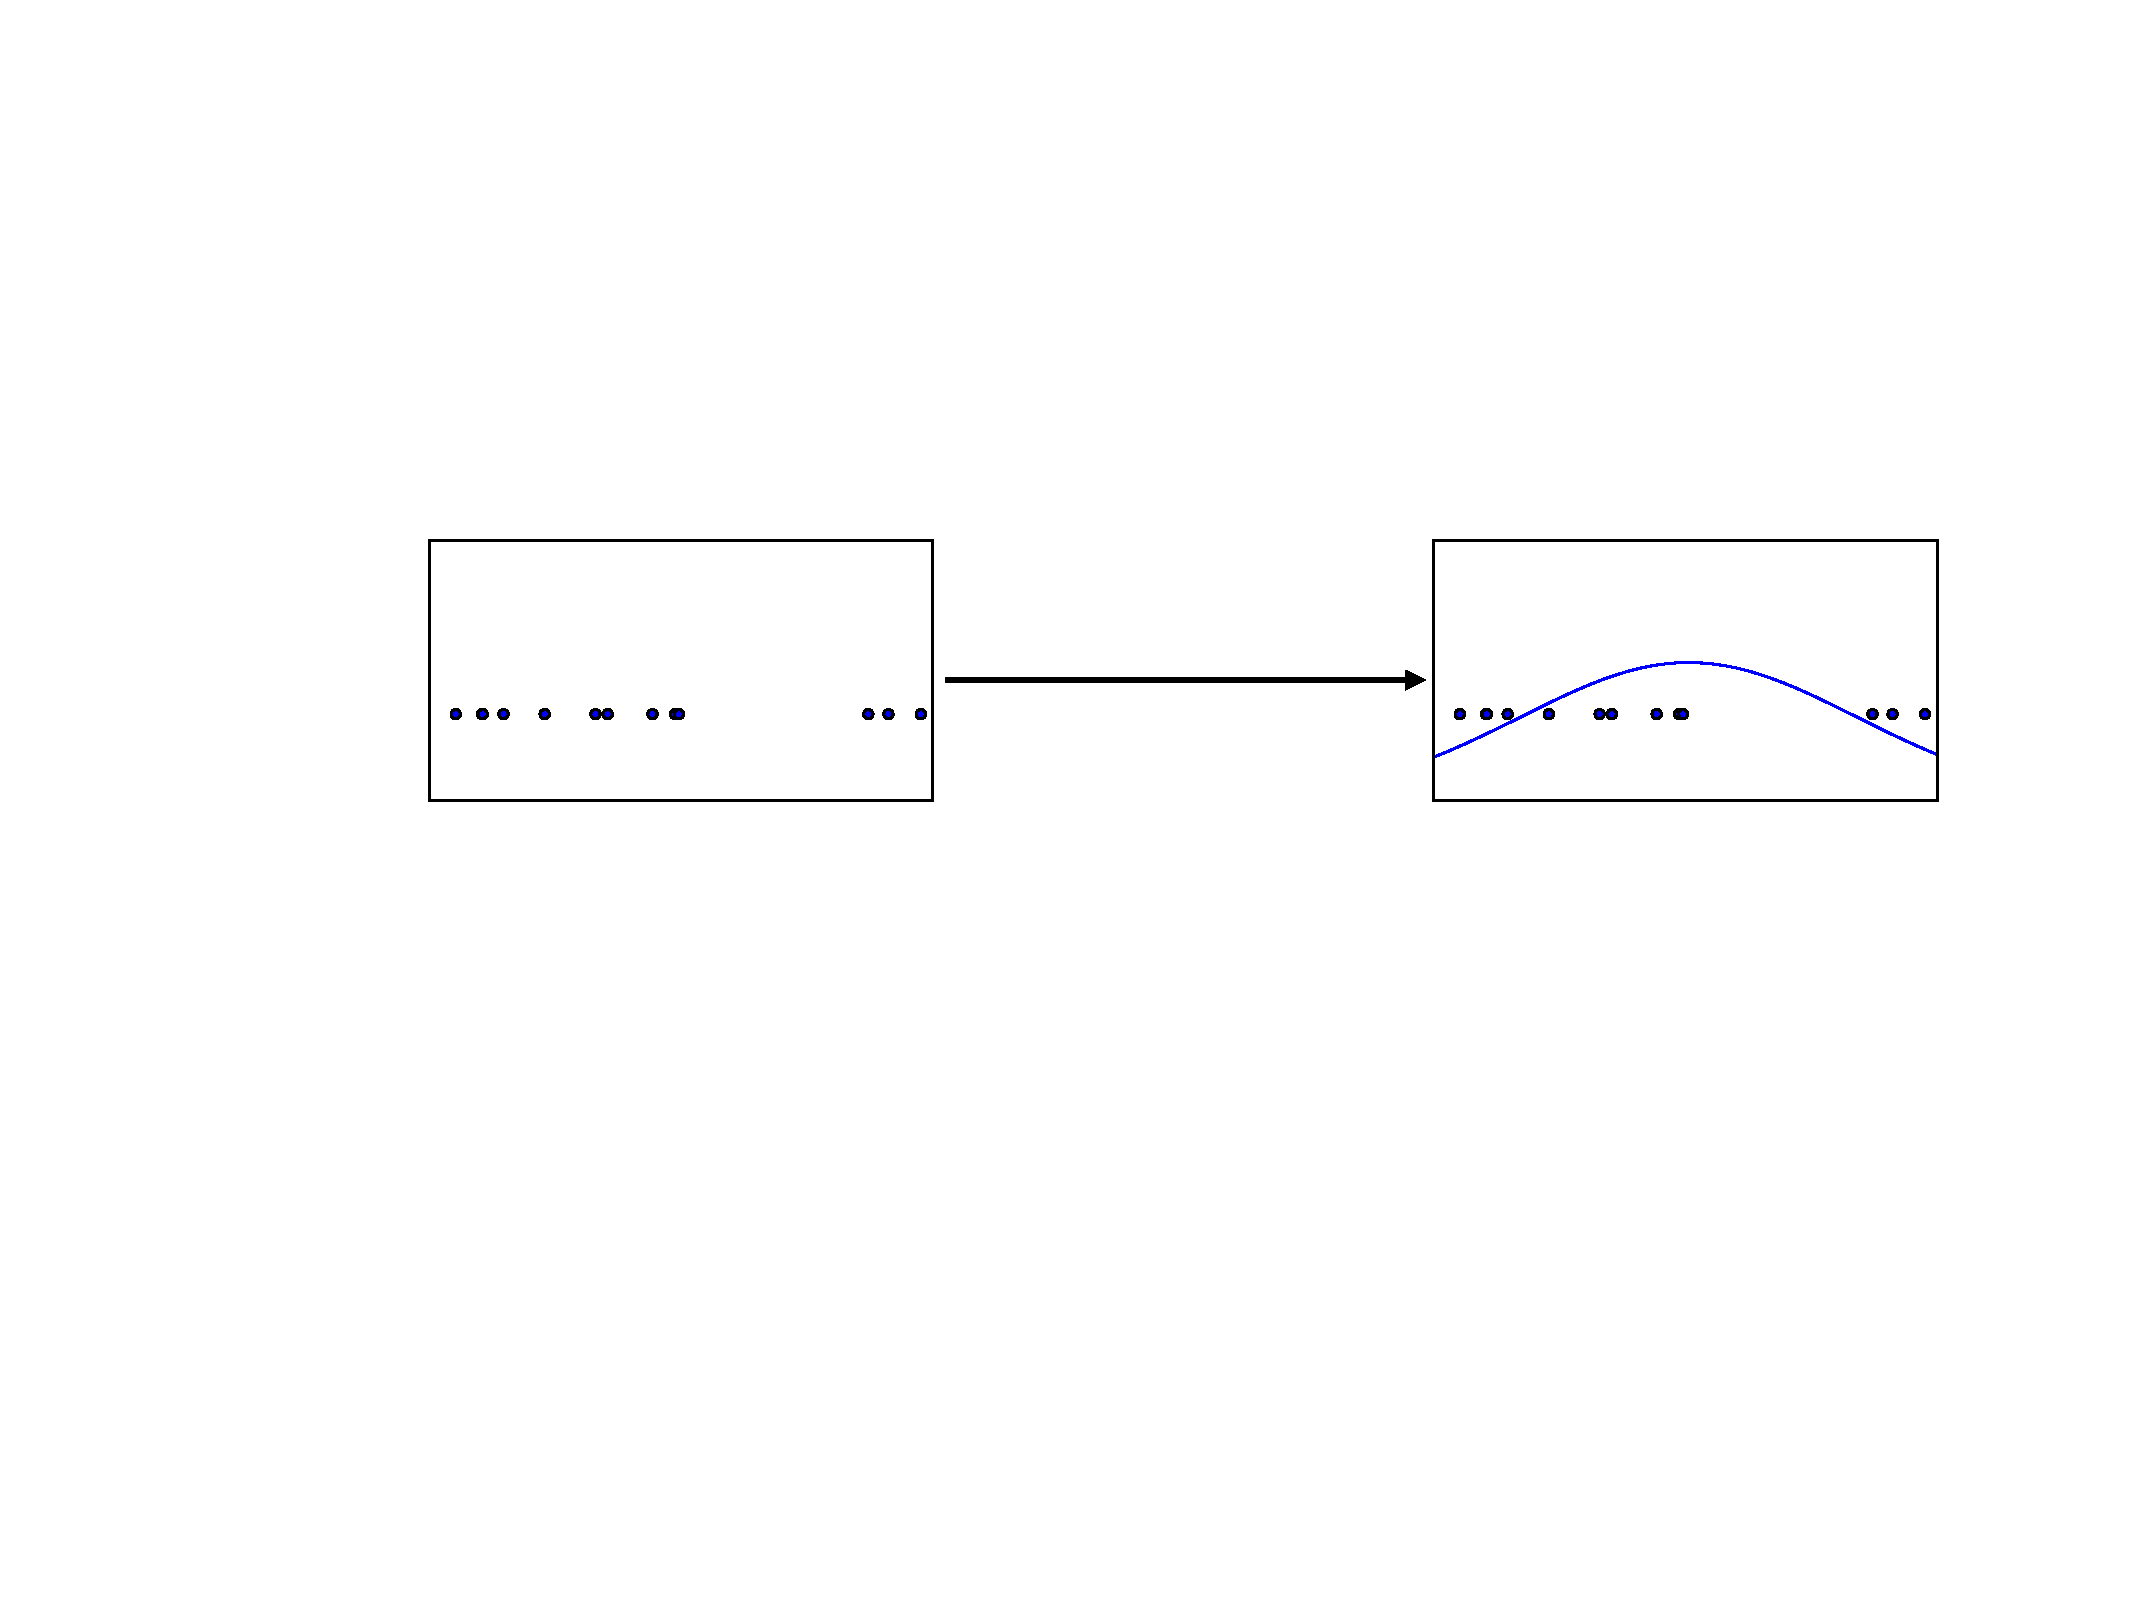
\includegraphics[width=\textwidth]{density.pdf}
\caption{Some generative models perform density estimation.
These models take a training set of examples drawn from an unknown
data-generating distribution $\pdata$ and return an estimate of that
distribution. The estimate $\pmodel$ can be evaluated for a particular
value of $\vx$ to obtain an estimate $\pmodel(\vx)$ of the true
density $\pmodel(\vx)$.
This figure illustrates the process for a collection of samples of
one-dimensional data and a Gaussian model.
}
\label{fig:density}
\end{figure}

\begin{figure}
  \center
  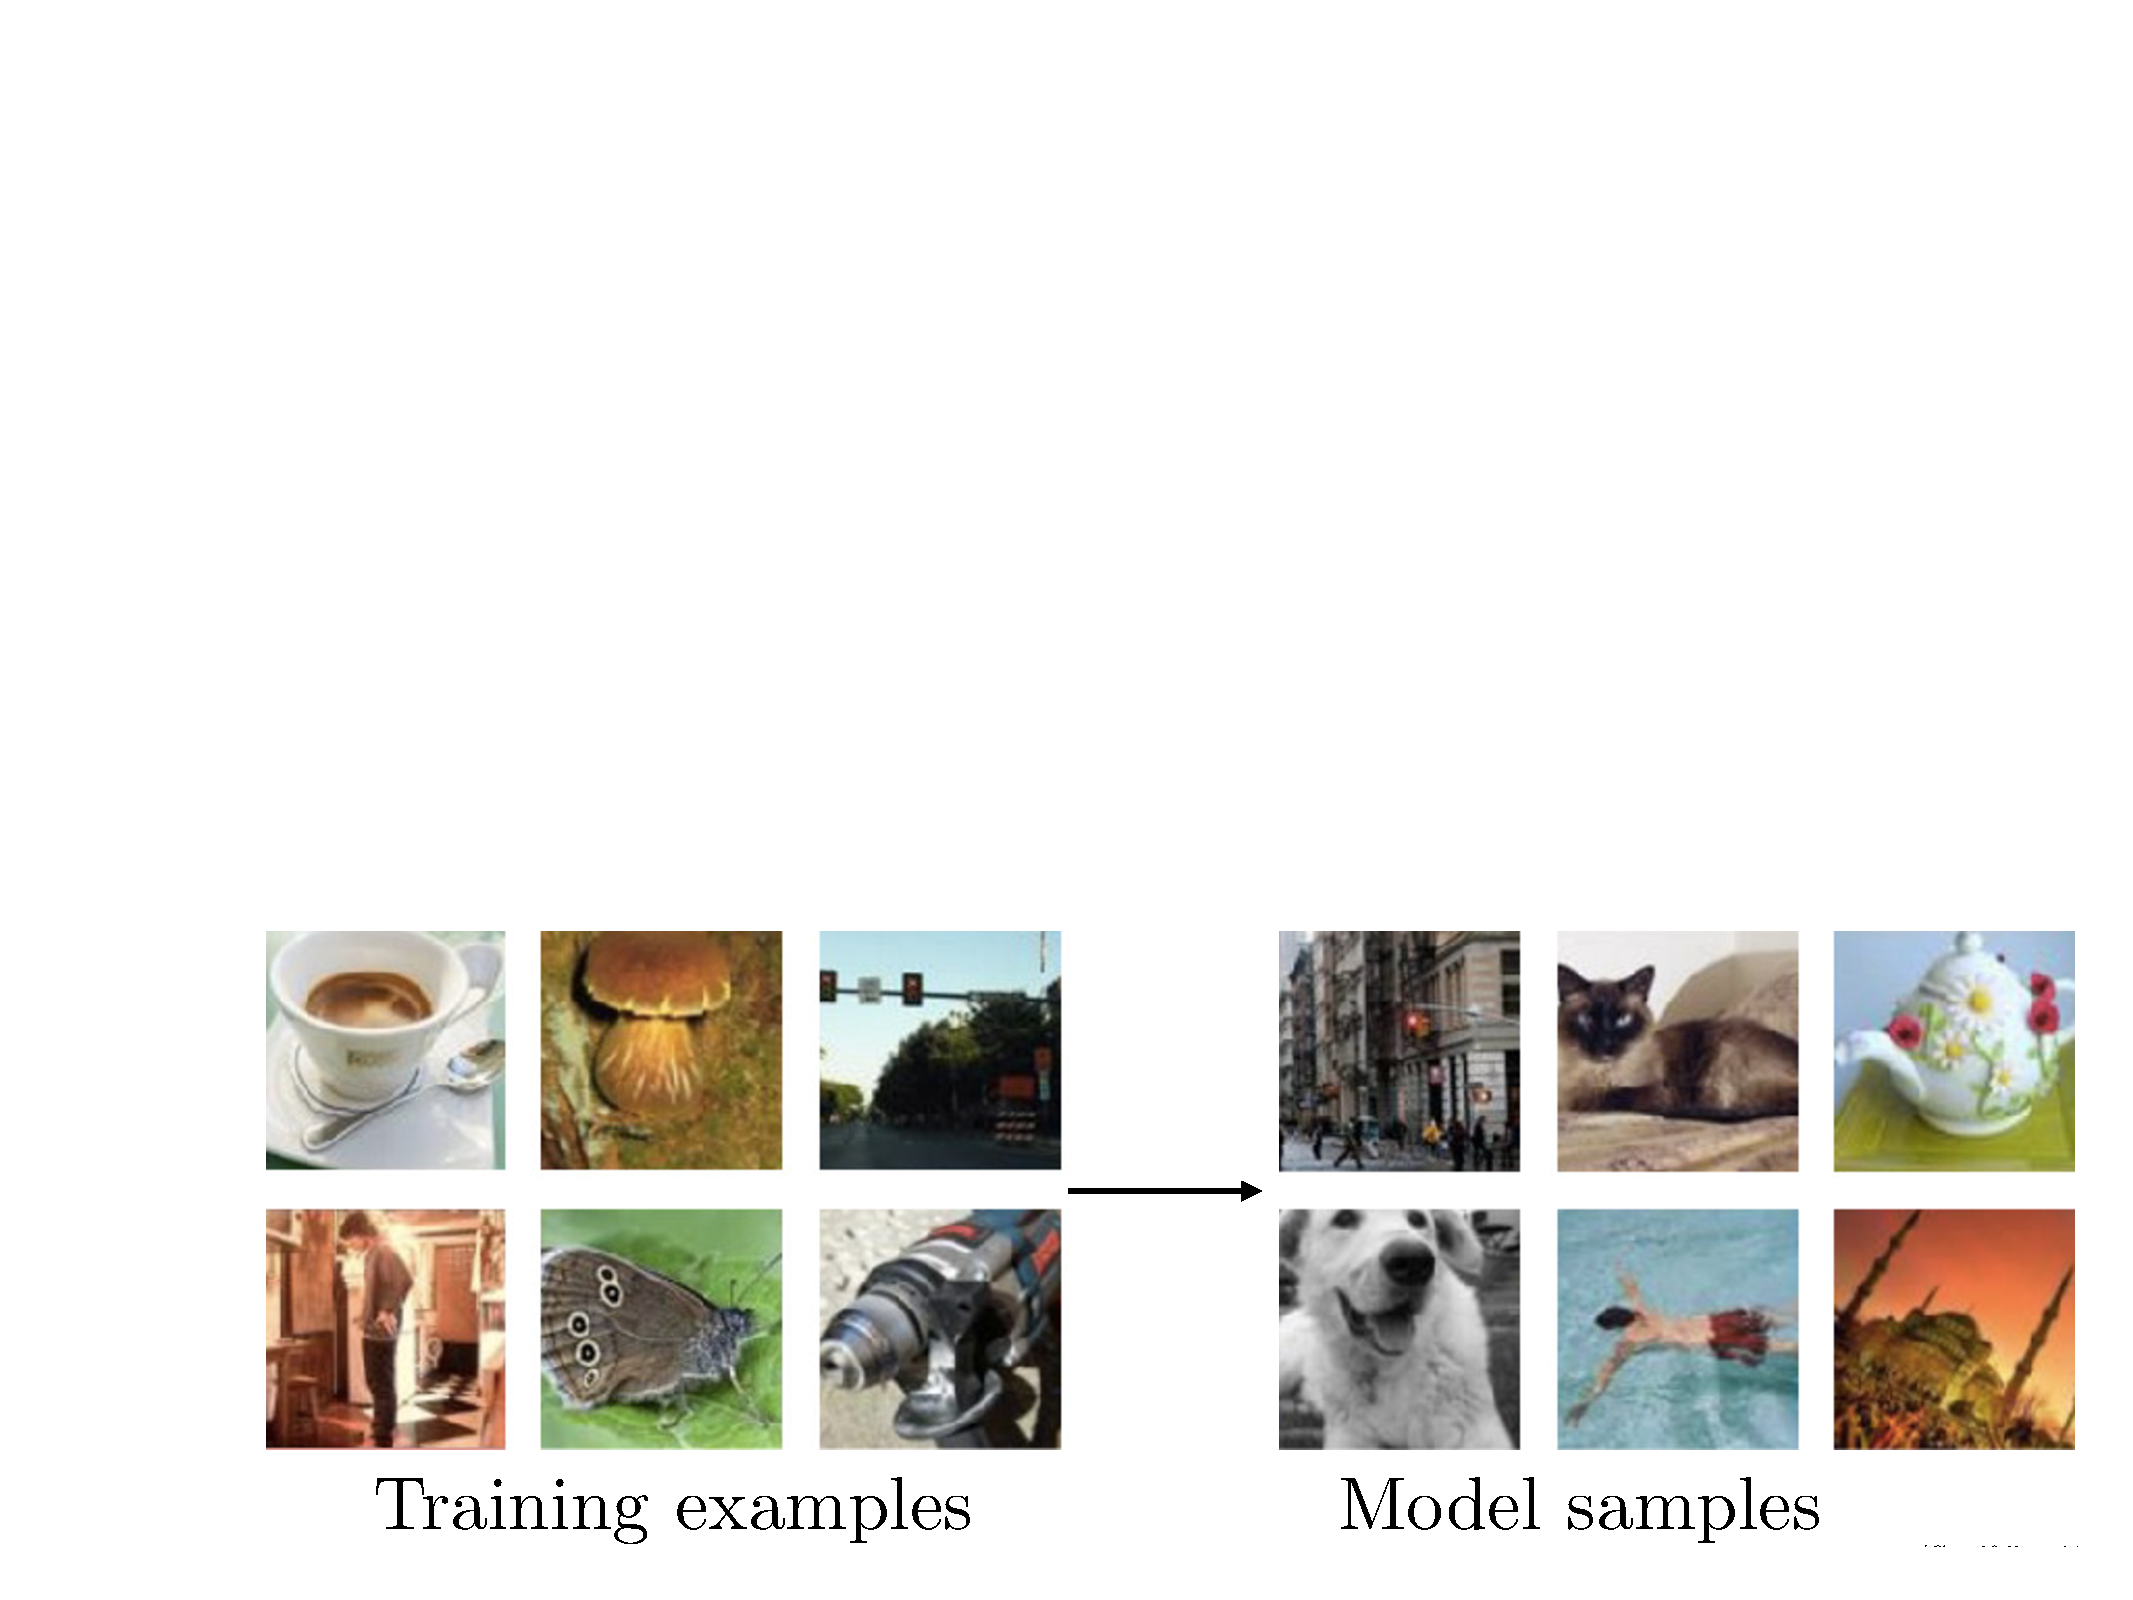
\includegraphics[width=\textwidth]{generative_machine.pdf}
  \caption{Some generative models are able to generate samples
    from the model distribution.
    In this illustration of the process, we show samples from
    the ImageNet \citep{imagenet_cvpr09,Deng2010,ILSVRCarxiv14} 
    dataset.
    An ideal generative model would be able to train on examples
    as shown on the left and then create more examples from the
    same distribution as shown on the right.
    At present, generative models are not yet advanced enough to
    do this correctly for ImageNet, so for demonstration purposes
    this figure uses actual ImageNet data to illustrate what an
    ideal generative model would produce.
  }
  \label{fig:generative_machine}
\end{figure}


\section{Why study generative modeling?}
\label{sec:why}

One might legitimately wonder why generative models are worth studying,
especially generative models that are only capable of generating data
rather than providing an estimate of the density function.
After all, when applied to images, such models seem to merely provide
more images, and the world has no shortage of images.

There are several reasons to study generative models, including:
\begin{itemize}

\item Training and sampling from generative models is an excellent test
of our ability to represent and manipulate high-dimensional probability
distributions.
High-dimensional probability distributions are important objects in a
wide variety of applied math and engineering domains.

\item Generative models can be incorporated into reinforcement learning in several
  ways.
  Reinforcement learning algorithms can be divided into two categories;
  model-based and model-free, with model-based algorithms being those that
  contain a generative model.
  Generative models of time-series data can be used to simulate possible
futures. Such models could be used for planning and for reinforcement learning
in a variety of ways.
A generative model used for planning can learn a conditional distribution over
future states of the world, given the current state of the world and hypothetical
actions an agent might take as input.
The agent can query the model with different potential actions and choose actions
that the model predicts are likely to yield a desired state of the world.
For a recent example of such a model, see \citet{finn2016unsupervised},
and for a recent example of the use of such a model for planning,
see \citet{finn2016deep}. 
Another way that generative models might be used for reinforcement learning is
to enable learning in an imaginary environment, where mistaken actions do not
cause real damage to the agent.
Generative models can also be used to guide exploration by keeping track of
how often different states have been visited or different actions have been
attempted previously.
Generative models, and especially GANs, can also be used for inverse reinforcement
learning.
Some of these connections to reinforcement learning are described further in
TODO.

\item Generative models can be trained with missing data and can provide predictions
  on inputs that are missing data.
  One particularly interesting case of missing data is {\em semi-supervised learning},
  in which the labels for many or even most training examples are missing.
  Modern deep learning algorithms typically require extremely many labeled examples
  to be able to generalize well.
  Semi-supervised learning is one strategy for reducing the number of labels.
  The learning algorithm can improve its generalization by studying a large number
  of unlabeled examples which, which are usually easier to obtain.
  Generative models, and GANs in particular, are able to perform semi-supervised
  learning reasonably well. This is described further in TODO.

\item Generative models, and GANs in particular, enable machine learning to work with
  {\em multi-modal} outputs.
  For many tasks, a single input may correspond to many different correct answers,
  each of which is acceptable.
Some traditional means of training machine learning models, such as minimizing the
mean squared error between a desired output and the model's predicted output, are
not able to train models that can produce multiple different correct answers.
One example of such a scenario is predicting the next frame in a video, as shown
in \figref{fig:lotter}.

\item Finally, many tasks intrinsically require realitic generation of samples from
  some distribution.
\end{itemize}

\begin{figure}
\centering
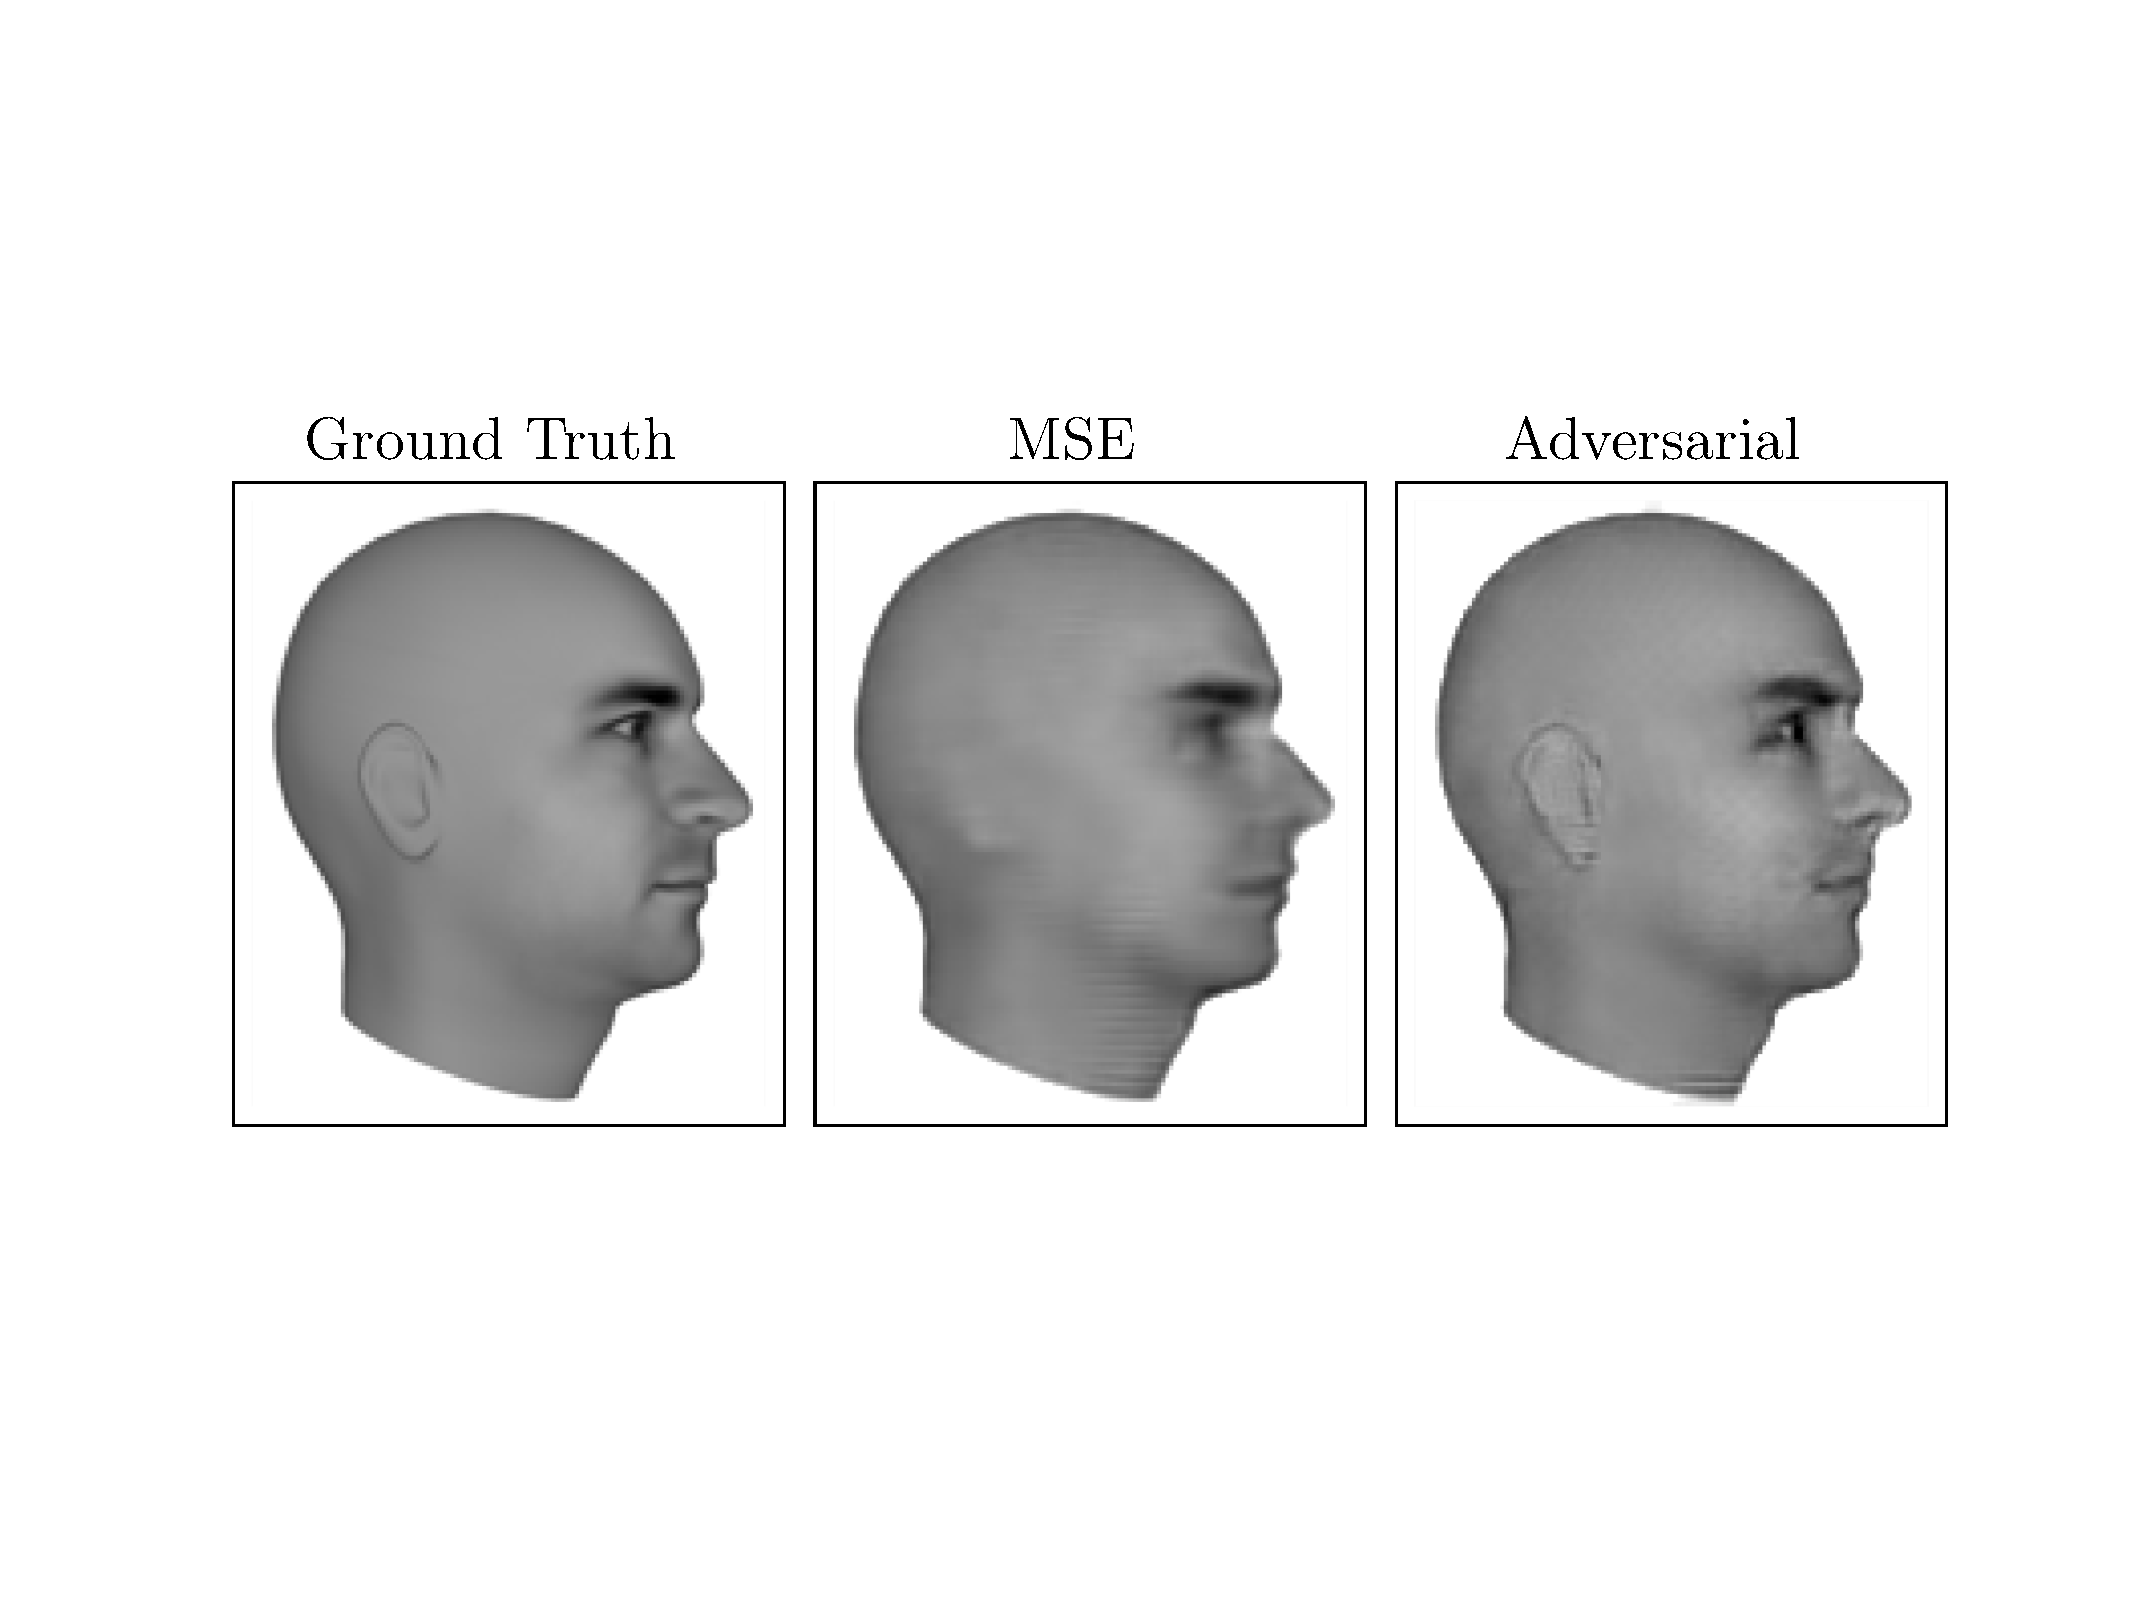
\includegraphics[width=\textwidth]{lotter.pdf}
\caption{
\citet{lotter2015unsupervised} provide an excellent illustration of the importance
of being able to model multi-modal data.
In this example, a model is trained to predict the next frame in a video sequence.
The video depicts a computer rendering of a moving 3D model of a person's head.
The image on the left shows an example of an actual frame of video, which the model
would ideally predict.
The image in the center shows what happens when the model is trained using mean
squared error between the actual next frame and the model's predicted next frame.
The model is forced to choose a single answer for what the next frame will look like.
Because there are many possible futures, corresponding to slightly different positions
of the head, the single answer that the model chooses corresponds to an average over
many slightly different images.
This causes the ears to practically vanish and the eyes to become blurry.
Using an additional GAN loss, the image on the right is able to understand that there
are many possible outputs, each of which is sharp and recognizable as a realistic,
detailed image.
}
  \label{fig:lotter}
\end{figure}

Examples of some of these tasks that intrinsically require the generation of good
samples include:
\begin{itemize}
  \item {\em Single image super-resolution}: In this task, the goal is to take a
    low-resolution image and synthesize a high-resolution equivalent.
    Generative modeling is required because this task requires the model to impute
    more information into the image than was originally there in the input.
    There are many possible high-resolution images corresponding to the low-resolution
    image.
    The model should choose an image that is a sample from the probability distribution
    over possible images.
    Choosing an image that is the average of all possible images would yield a result
    that is too blurry to be pleasing.
    See \figref{fig:superres}.

  \item Tasks where the goal is to create art.
    Two recent projects have both demonstrated that generative models, and in particular,
    GANs, can be used to create interactive programs that assist the user in creating
    realistic images that correspond to rough scenes in the user's imagination.
    See \figref{fig:igan} and \figref{fig:ian}.

\end{itemize}

\begin{figure}
  \centering
  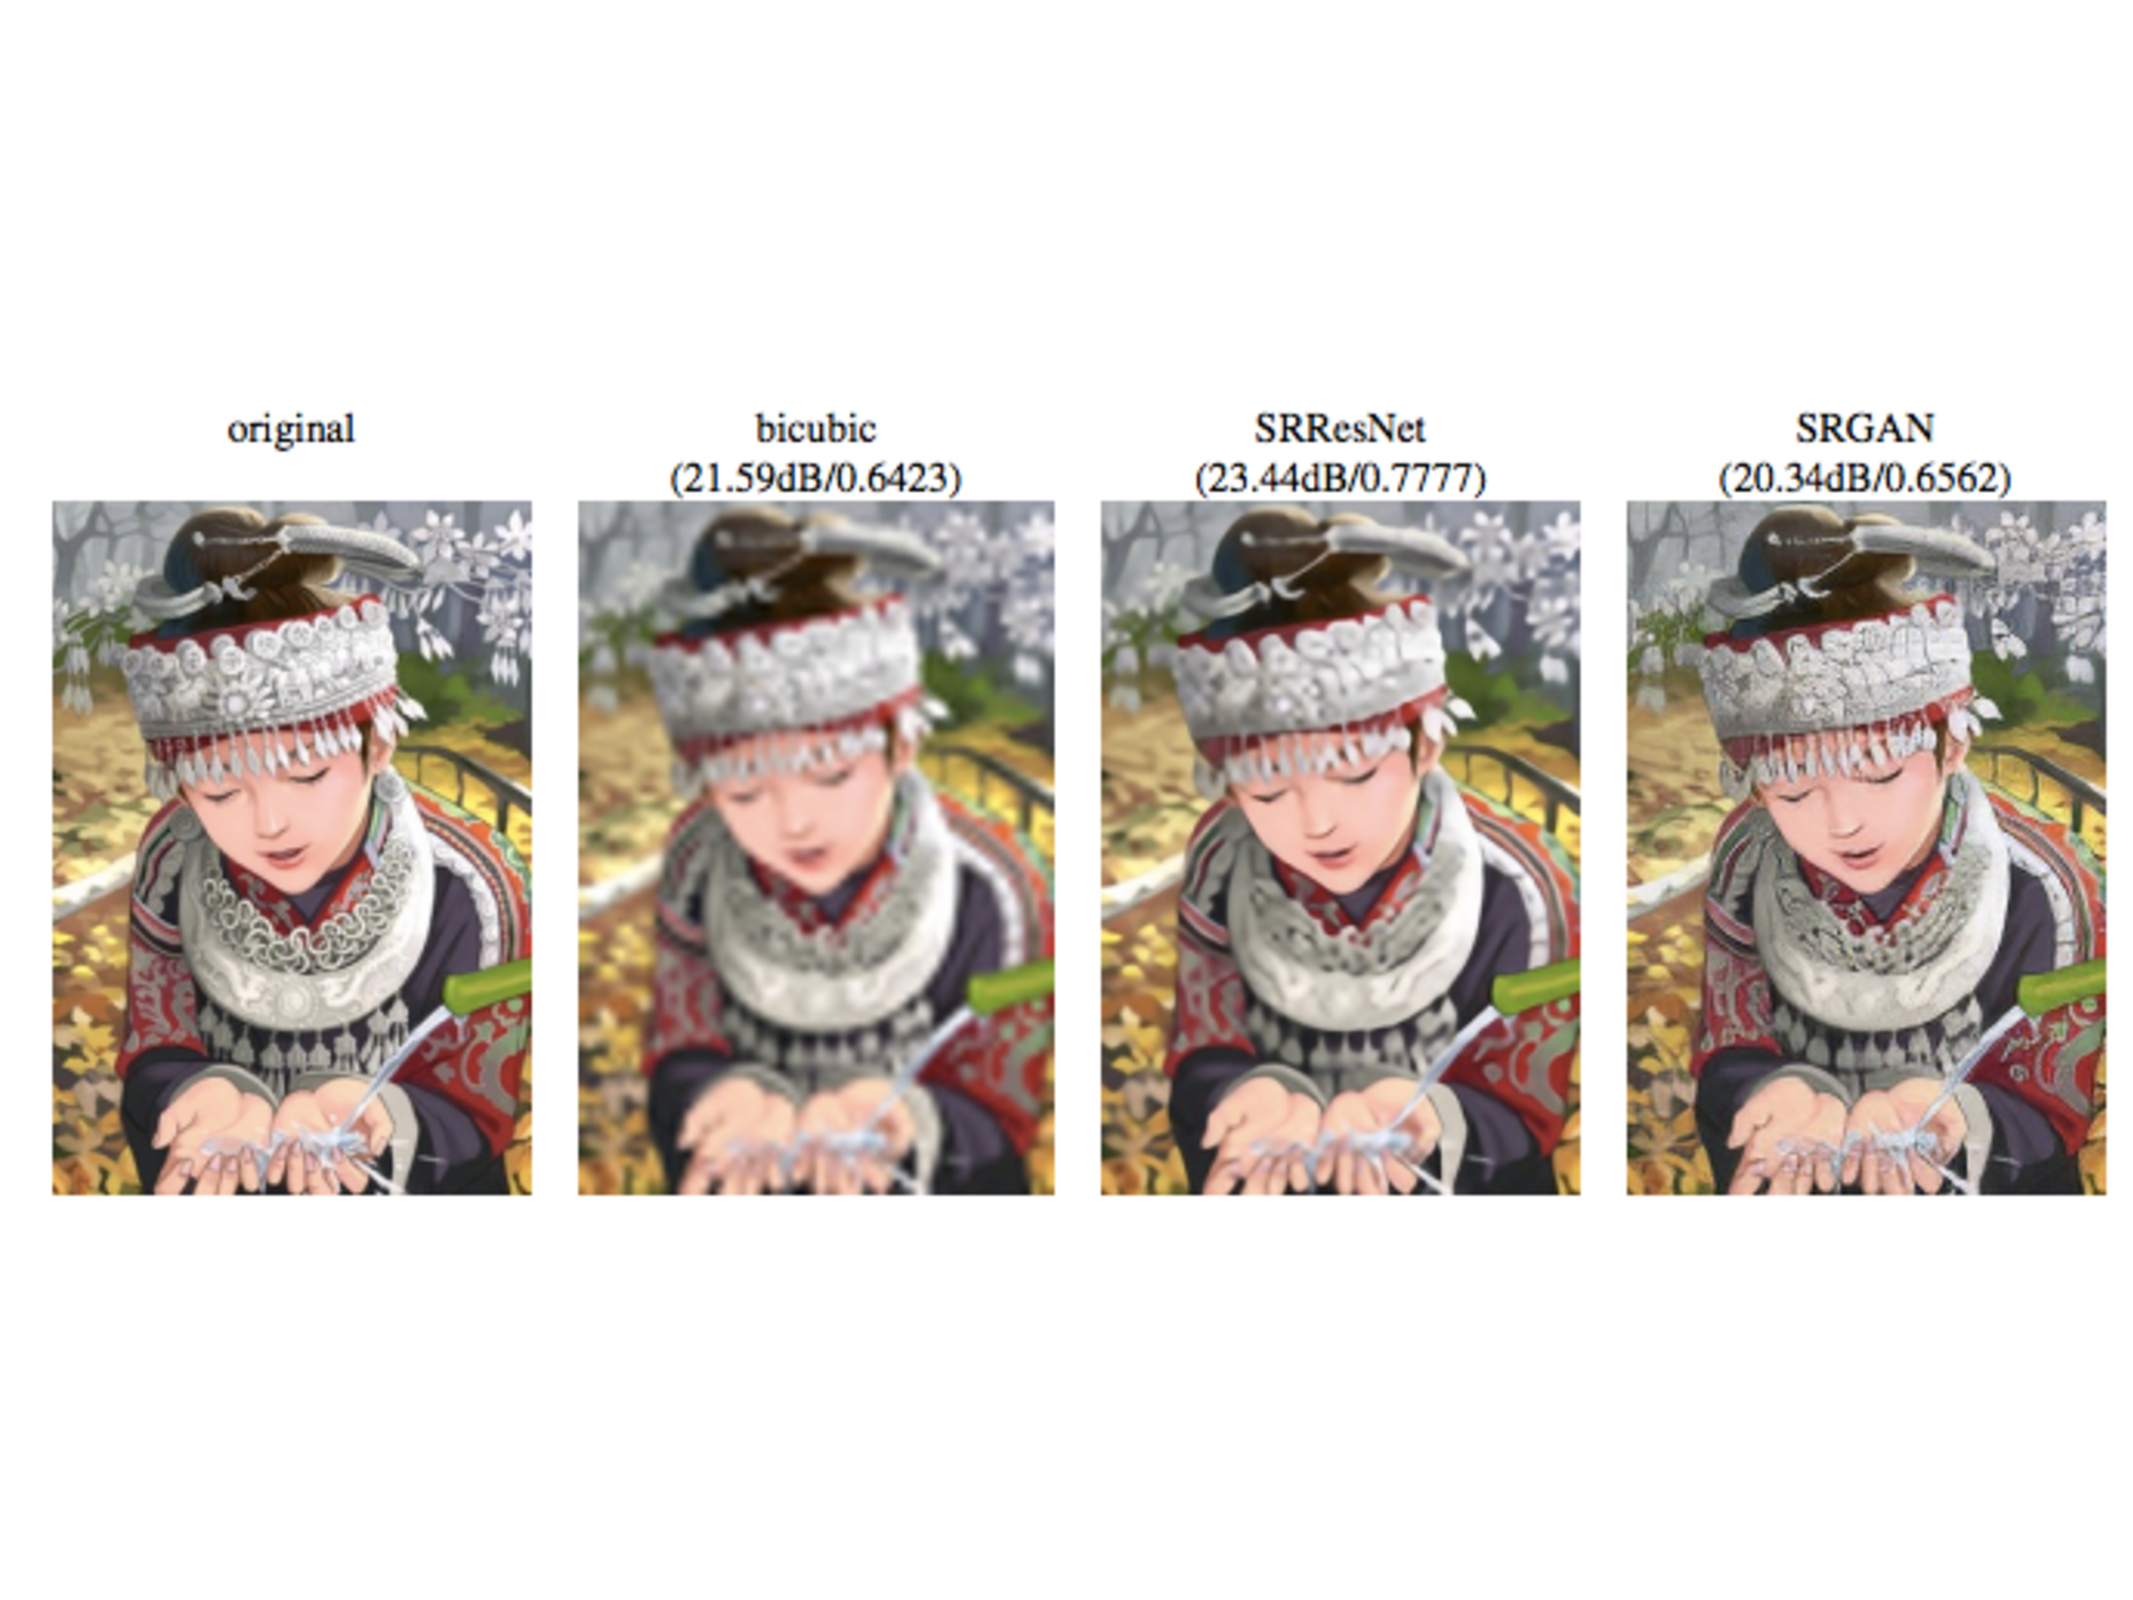
\includegraphics[width=\textwidth]{superres}
  \caption{
\citet{Ledig16} demonstrate excellent single-image superresolution results that show
the benefit of using a generative model trained to generate realistic samples from
 a multimodal distribution.
 The leftmost image is an original high-resolution image.
 It is then downsampled to make a low-resolution image, and different methods
 are used to attempt to recover the high-resolution image.
 The bicubic method is simply an interpolation method that does not use 
 the statistics of the training set at all.
 SRResNet is a neural network trained with mean squared error.
 SRGAN is a GAN-based neural network that improves over SRGAN because it is able
 to understand that there are multiple correct answers, rather than averaging
 over many answers to impose a single best output.
  }
  \label{fig:superres}
\end{figure}

\begin{figure}
  \centering
  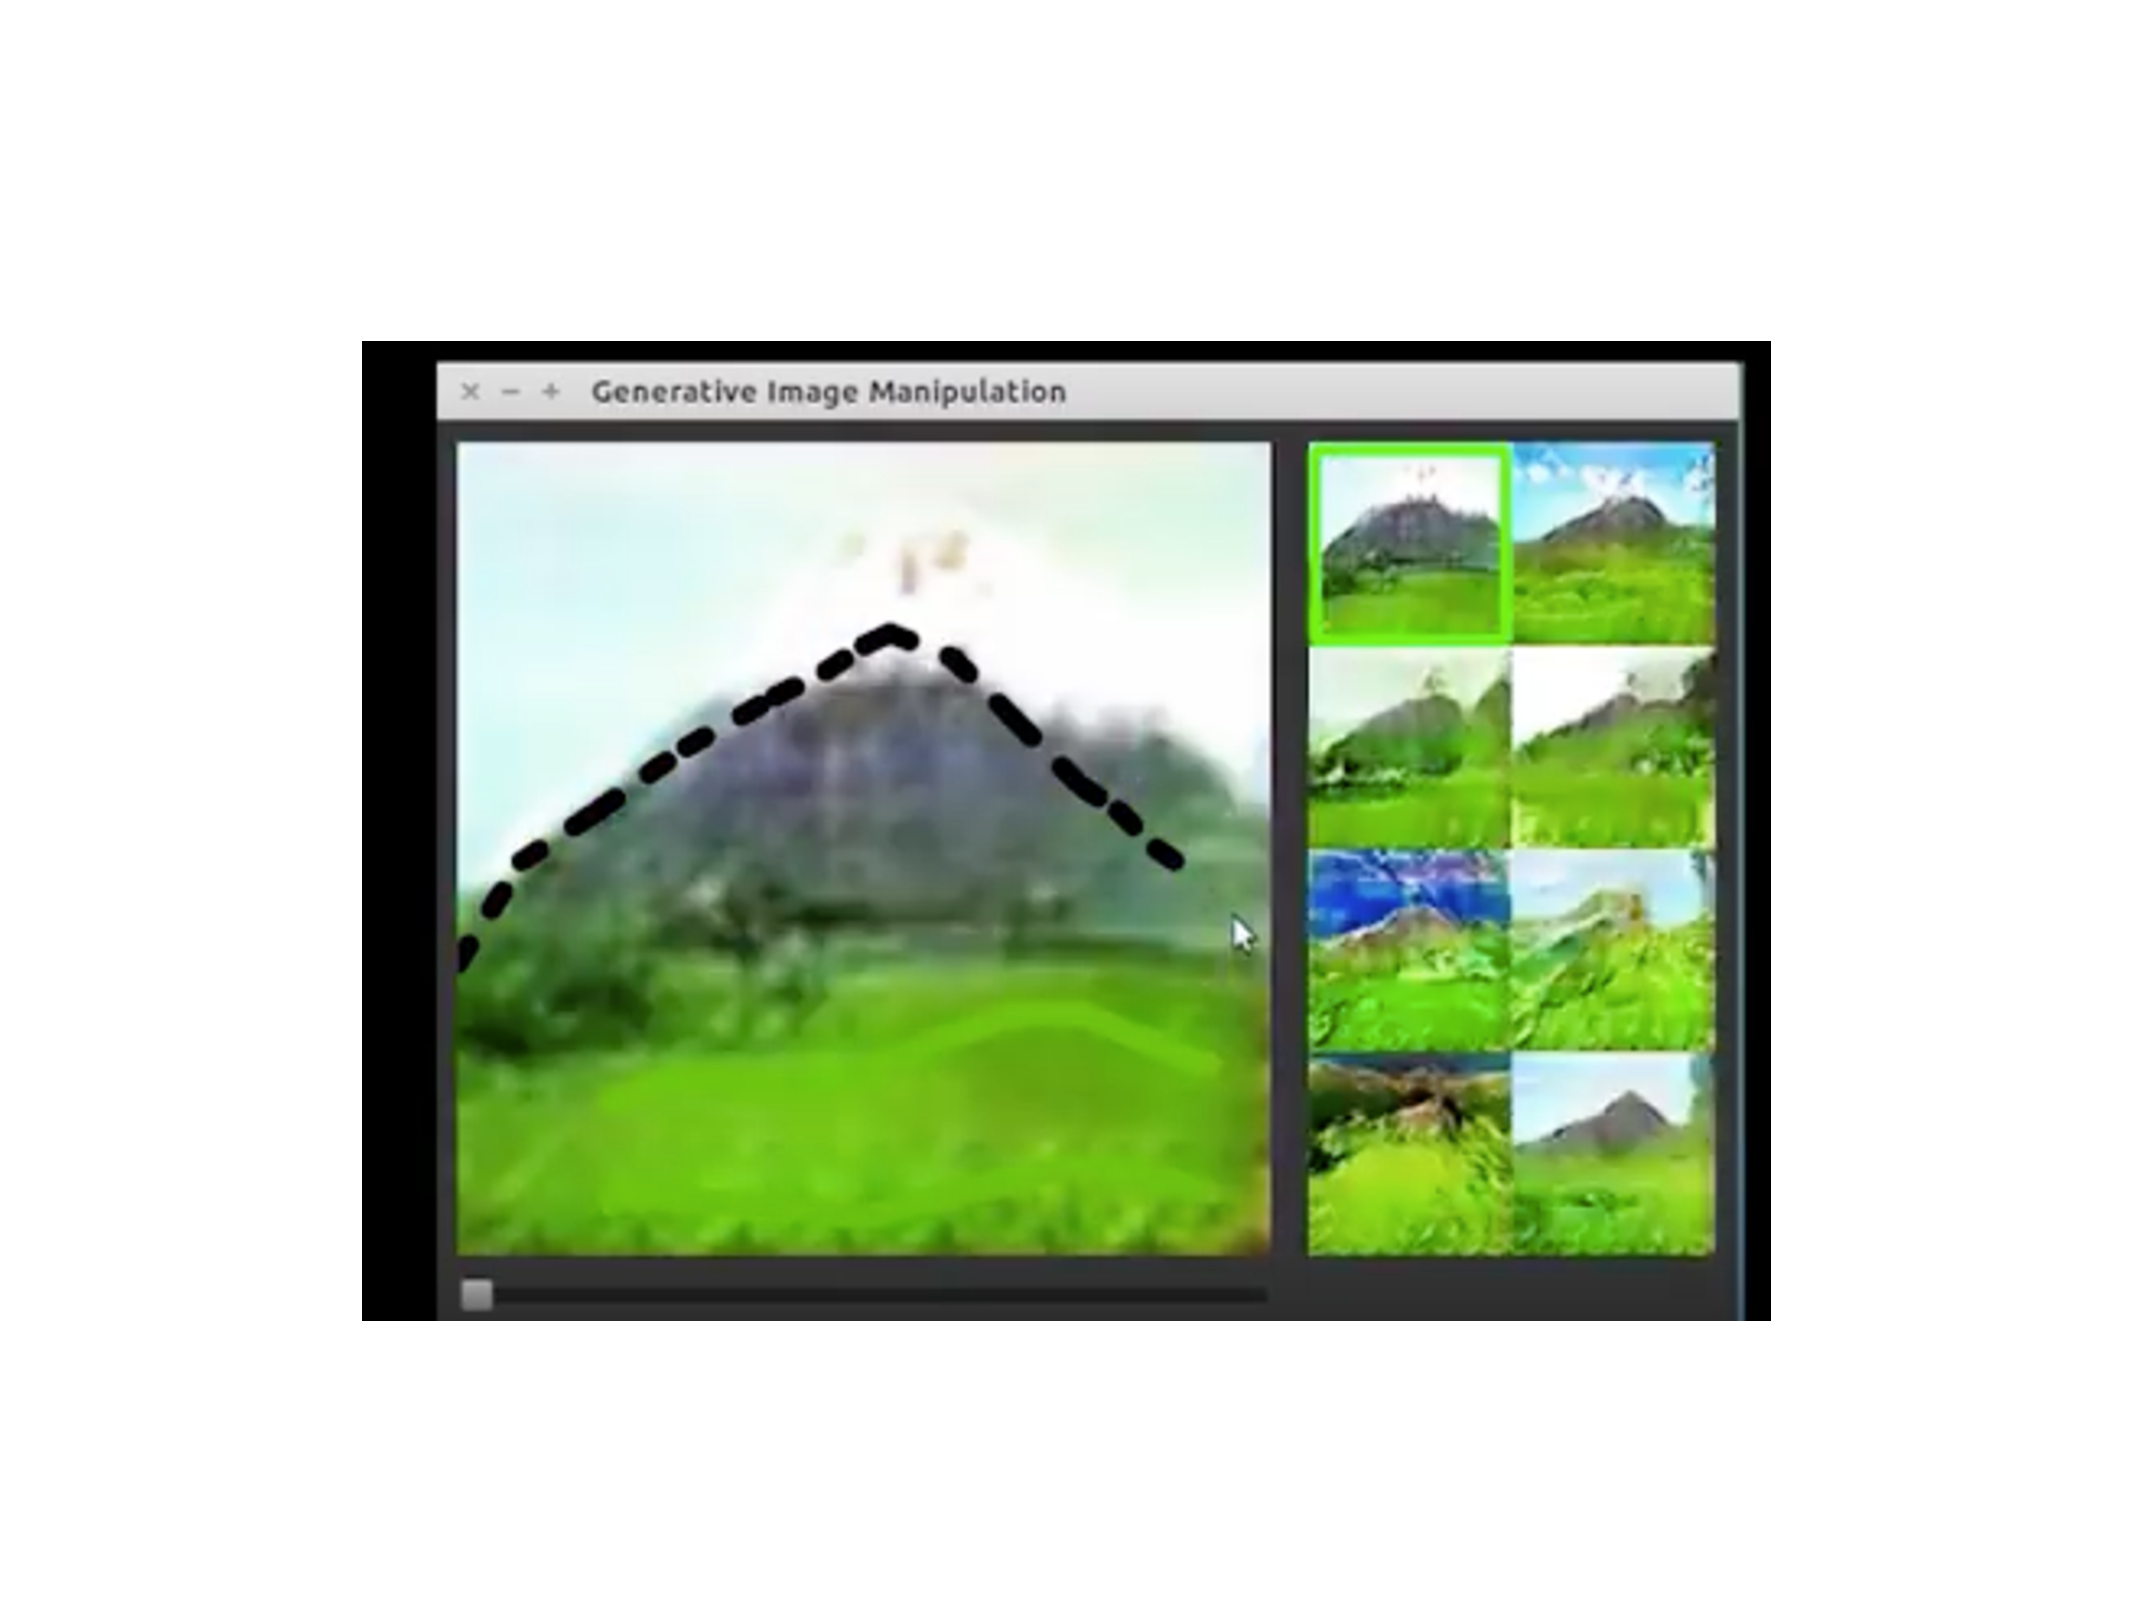
\includegraphics[width=\textwidth]{igan}
  \caption{
TODOcite developed an interactive application called {\em interactive generative adversarial networks}
(iGAN). 
A user can draw a rough sketch of an image, and iGAN uses a GAN to produce the most similar
realistic image.
In this example, a user has scribbled a few green lines that iGAN has converted into a grassy
field, and the user has drawn a black triangle that iGAN has turned into a detailed mountain.
Applications that create art are one of many reasons to study generative models that create
images.
A video demonstration of iGAN is available at the following URL:
\url{https://www.youtube.com/watch?v=9c4z6YsBGQ0}
}
  \label{fig:igan}
\end{figure}


\begin{figure}
  \centering
  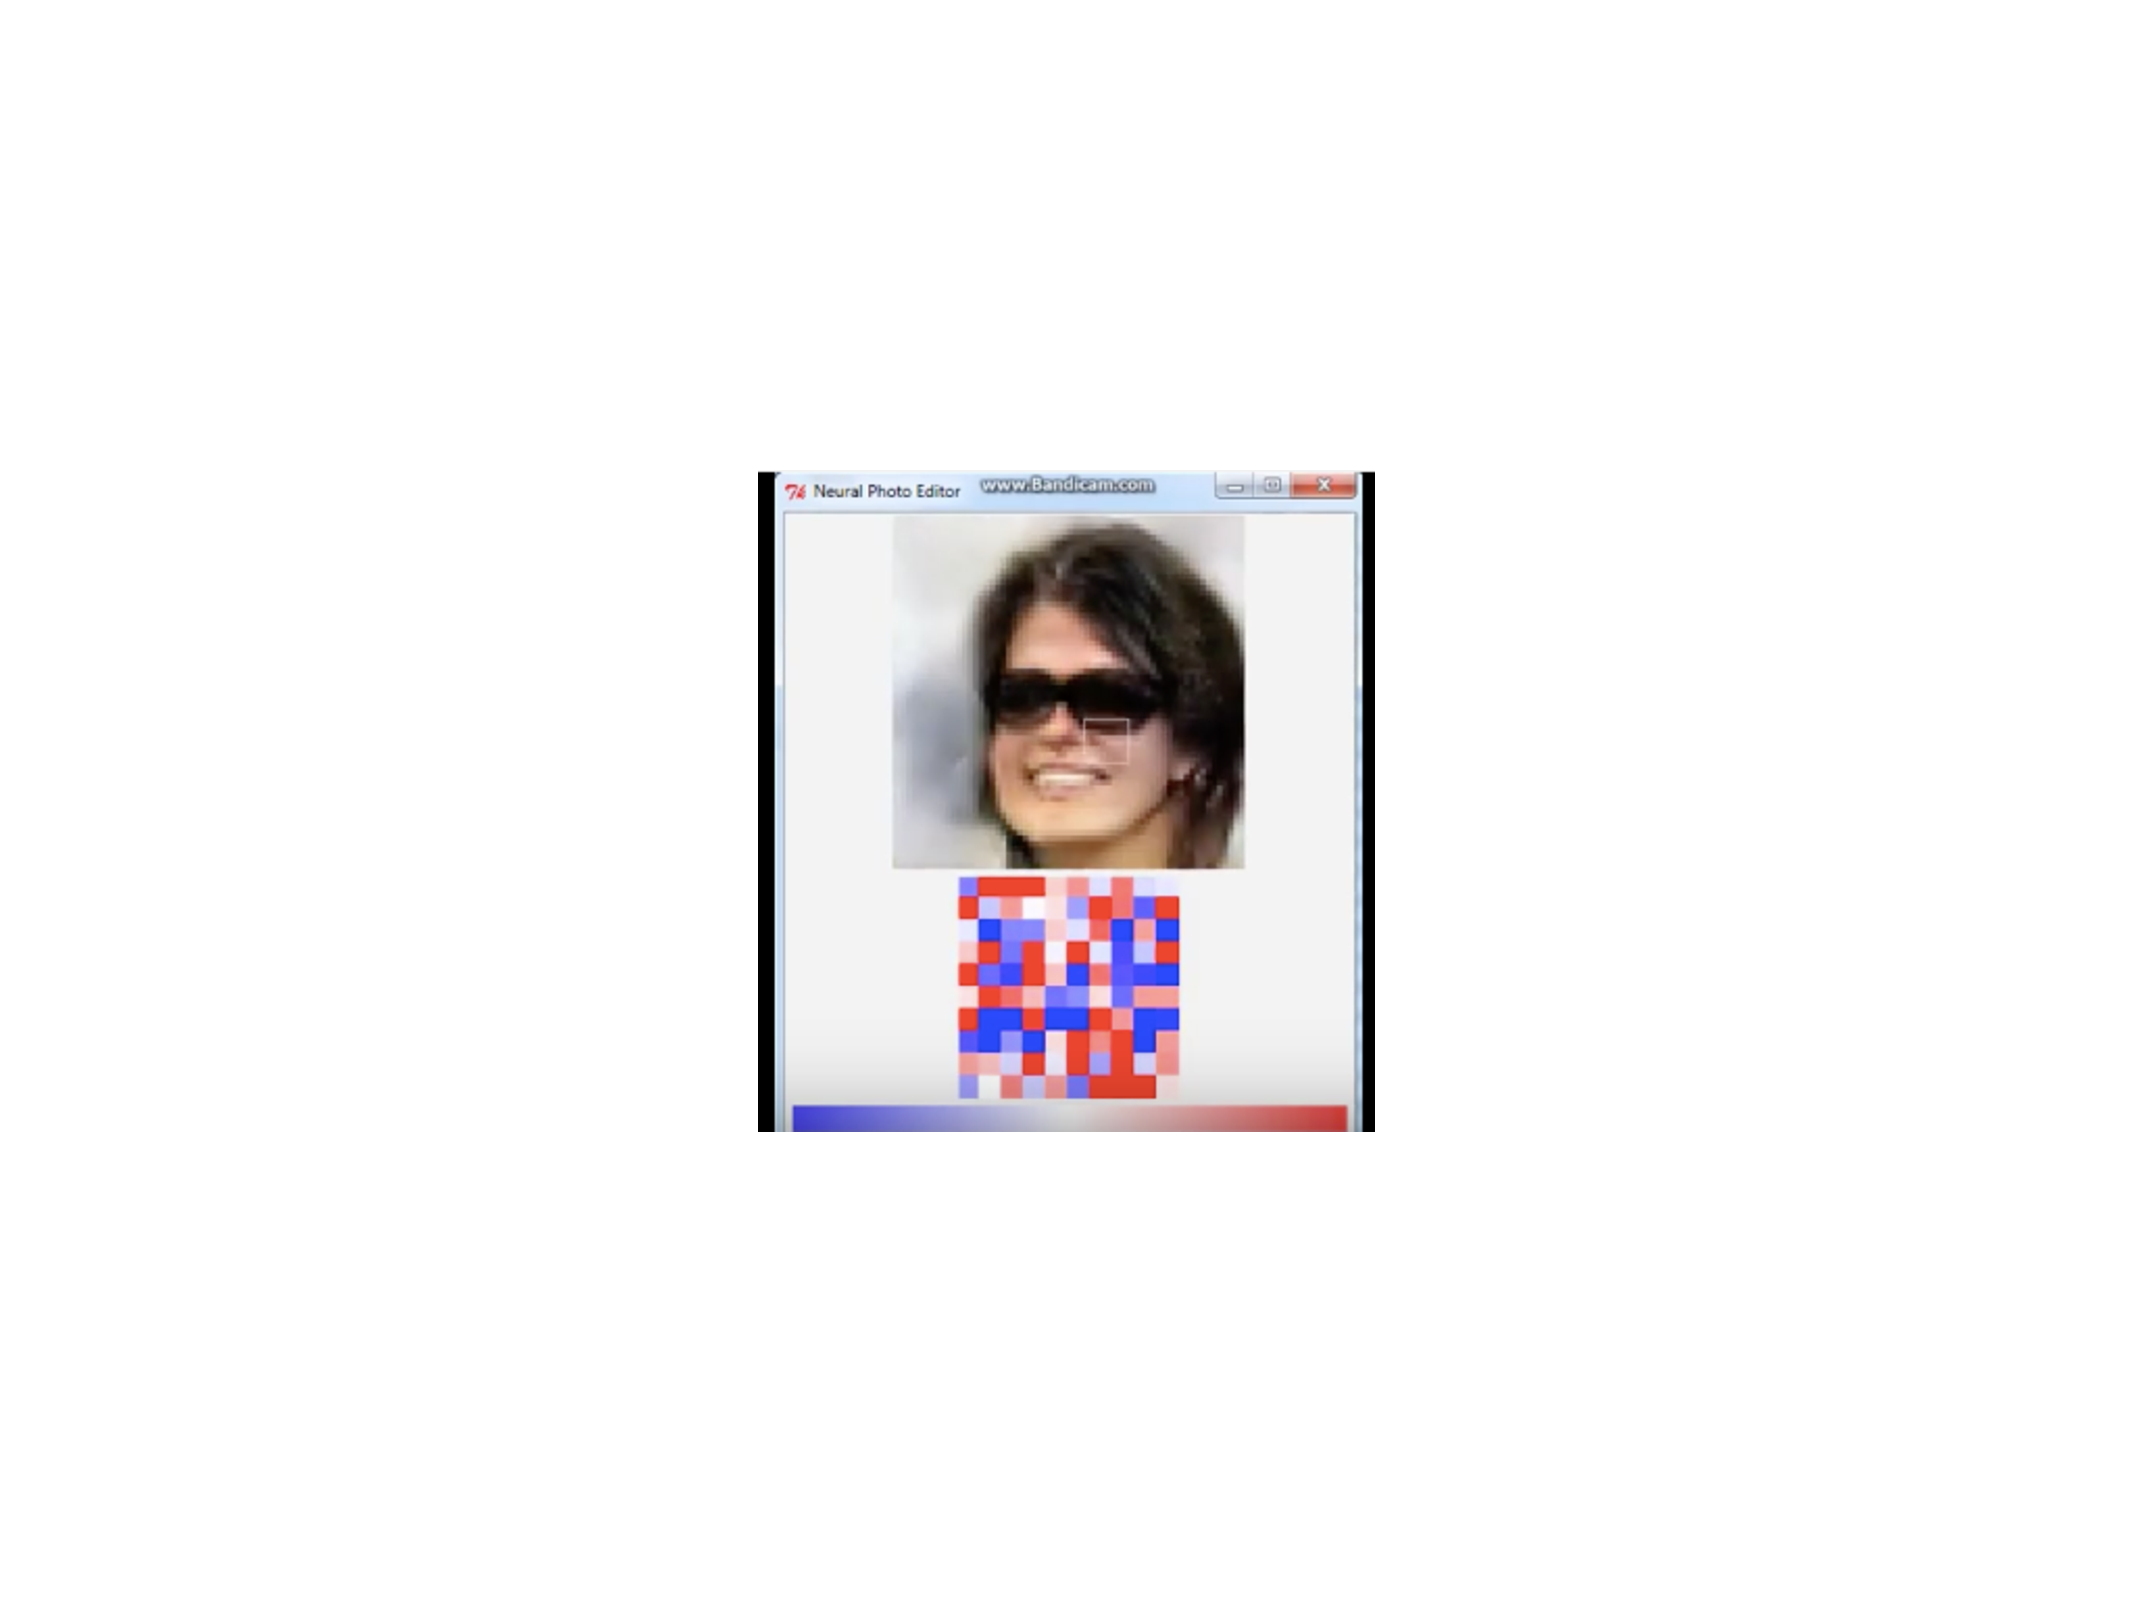
\includegraphics[width=\textwidth]{ian}
  \caption{
    TODOcite developed {\em interactive adversarial networks} (IAN).
    The user paints rough modifications to a photo, such as painting
    with black paint in an area where the user would like to add black
    hair, and IAN turns these rough paint strokes into photorealistic
    imagery matching the user's desires.
    Applications that enable a user to make realistic modifications to
    photo media are one of many reasons to study generative models
    that create images.
    A video demonstration of IAN is available at the following URL:
    \url{https://www.youtube.com/watch?v=FDELBFSeqQs}
  }
  \label{fig:ian}
\end{figure}

\section{How do generative models work? How do GANs compare to others?}
\label{sec:tree}

We now have some idea of what generative models can do and why it might be
desirable to build one.
Now we can ask: how does a generative model actually work? And in particular,
how does a GAN work, in comparison to other generative models?

\subsection{Maximum likelihood estimation}

To simplify the discussion somewhat, we will focus on generative models
that work via the principle of \newterm{maximum likelihood}.
Not every generative model uses maximum likelihood.
Some generative models do not use maximum likelihood by default, but
can be made to do so (GANs fall into this category).
By ignoring those models that do not use maximum likelihood, and
by focusing on the maximum likelihood version of models that do not
usually use maximum likelihood, we can eliminate some of the more 
distracting differences between different models.

The basic idea of maximum likelihood is to define a model that provides
an estimate of a probability distribution, parameterized by parameters
$\vtheta$.
We then refer to the \newterm{likelihood} as the probability that the model
assigns to the training data: $\prod_{i=1}^m \pmodel\left(\vx^{(i)}; \vtheta \right),$
for a dataset containing $m$ training examples $\vx^{(i)}$.

The principle of maximum likelihood simply says to choose the parameters for the model
that maximize the likelihood of the training data.
This is easiest to do in log space, where we have a sum rather than a product
over examples.
This sum simplifies the algebraic expressions for the derivatives of the likelihood
with respect to the models, and when implemented on a digital computer, is less
prone to numerical problems, such as underflow resulting from multiplying together
several very small probabilities.

\begin{align}
\vtheta^* =& \argmax_\vtheta \prod_{i=1}^m \pmodel\left(\vx^{(i)}; \vtheta \right) \\
  =& \argmax_\vtheta \log \prod_{i=1}&m \pmodel\left(\vx^{(i)}; \vtheta \right) \label{eq:log} \\
          =& \argmax_\vtheta \sum_{i=1}^m \log \pmodel\left(\vx^{(i)}; \vtheta \right).
\end{align}

In \eqref{eq:log}, we have used the property that $\argmax_v f(v) = \argmax_v \log f(v)$ for 
positive $v$, because the logarithm is a function that increases everywhere and does not change
the location of the maximum.

The maximum likelihood process is illustrated in \figref{fig:mle}.

We can also think of maximum likelihood estimation as minimizing the
\newterm{KL divergence} between the data generating distribution and the
model:
\[ \vtheta^* = \argmin_\vtheta \KL\left( \pdata(\vx) \Vert \pmodel(\vx ; \vtheta) \right). \]
If we were able to do this precisely, then if $\pdata$ lies within the family of distributions
$\pmodel(\vx ; \vtheta)$, the model would recover $\pdata$ exactly.
In practice, we do not have access to $\pdata$ itself, but only to a training set
consisting of $m$ samples from $\pdata$.
We uses these to define $\ptrain$, an \newterm{empirical distribution} that places mass only
on exactly those $m$ points, approximating $\pdata$.
Minimizing the KL divergence between $\ptrain$ and $\pmodel$ is exactly equivalent to maximizing
the log-likelihood of the training set.

\begin{figure}
\centering
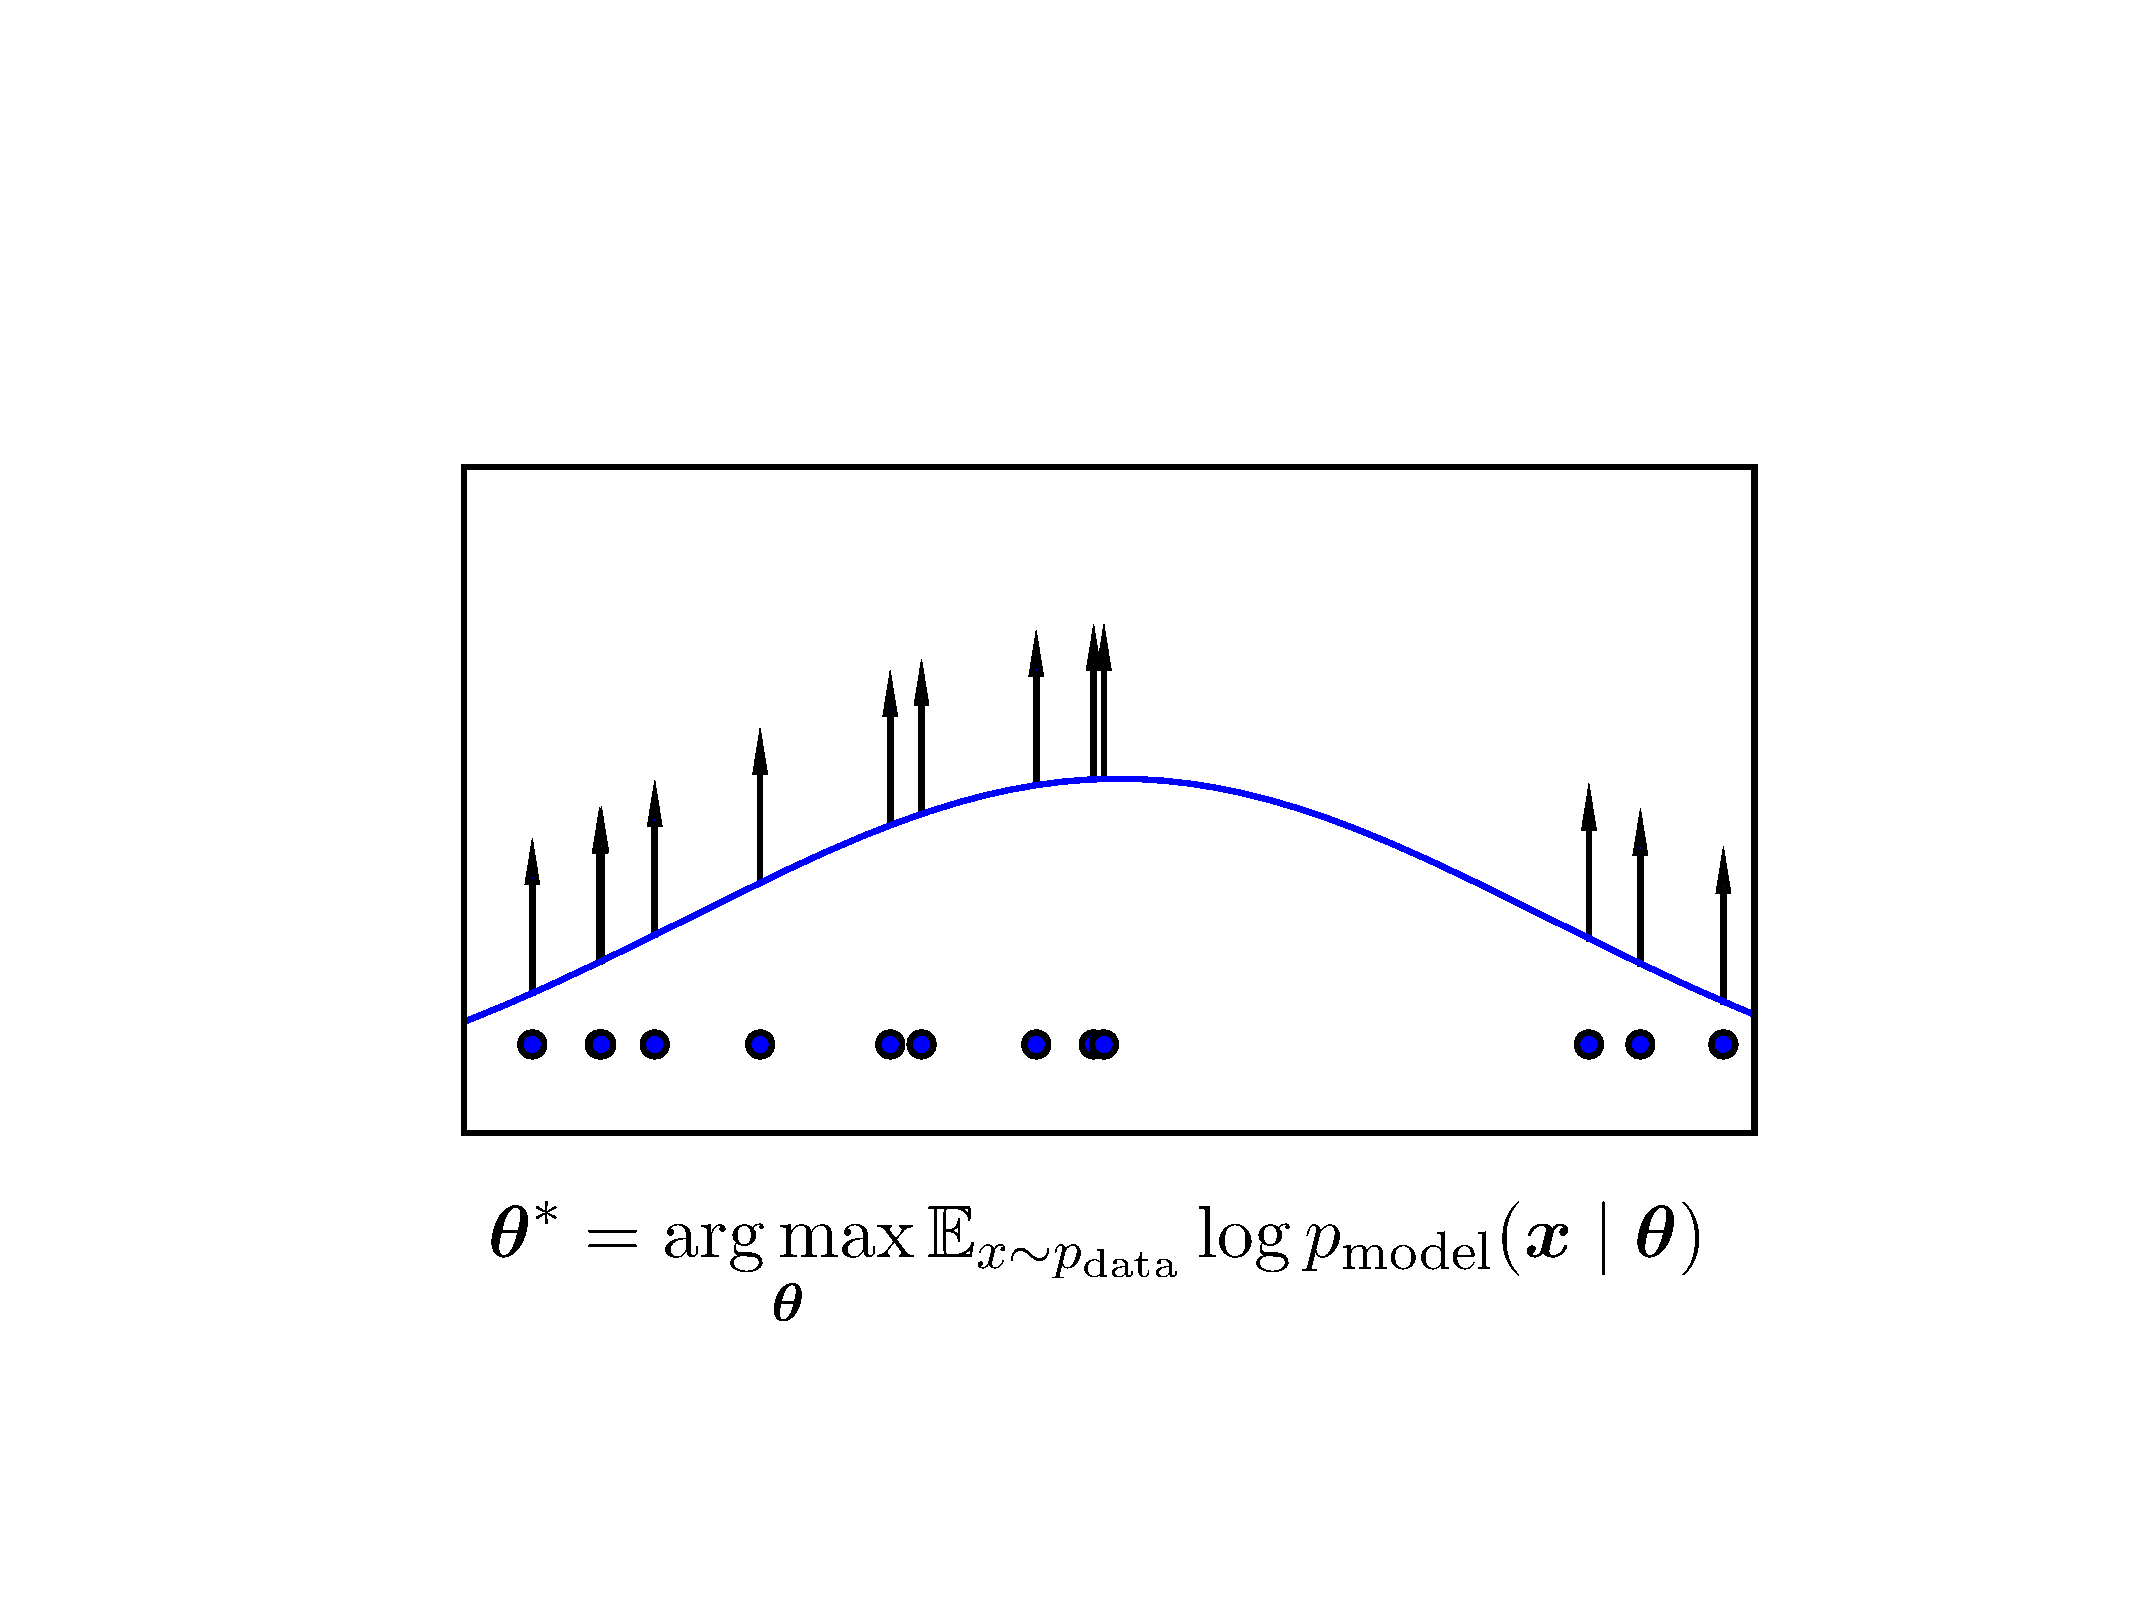
\includegraphics[width=\textwidth]{mle.pdf}
\caption{The maximum likelihood process consists of taking several samples from
  the data generating distribution to form a training set, then pushing up on the
  probability the model assigns to those points, in order to maximize the likelihood
  of the training data.
  This illustration shows how different data points push up on different parts of
  the density function for a Gaussian model applied to 1-D data.
  The fact that the density function must sum to $1$ means that we cannot simply
  assign infinite likelihood to all points; as one point pushes up in one place
  it inevitably pulls down in other places.
  The resulting density function balances out the upward forces from all the data
  points in different locations.
}
\label{fig:mle}
\end{figure}

For more information on maximum likelihood and other statistical estimators,
see chapter 5 of \citet{Goodfellow-et-al-2016}.


\subsection{A taxonomy of deep generative models}

If we restrict our attention to deep generative models that work by maximizing
the likelihood, we can compare several models by contrasting the ways that they
compute either the likelihood and its gradients, or approximations to these
quantities.
As mentioned earlier, many of these models are often used with principles other
than maximum likelihood, but we can examine the maximum likelihood variant of
each of them in order to reduce the amount of distracting differences between
the methods.
Following this approach, we construct the taxonomy shown in \figref{fig:tree}.
Every leaf in this taxonomic tree has some advantages and disadvantages.
GANs were designed to avoid many of the disadvantages present in pre-existing
nodes of the tree, but also introduced some new disadvantages.

\begin{figure}
\centering
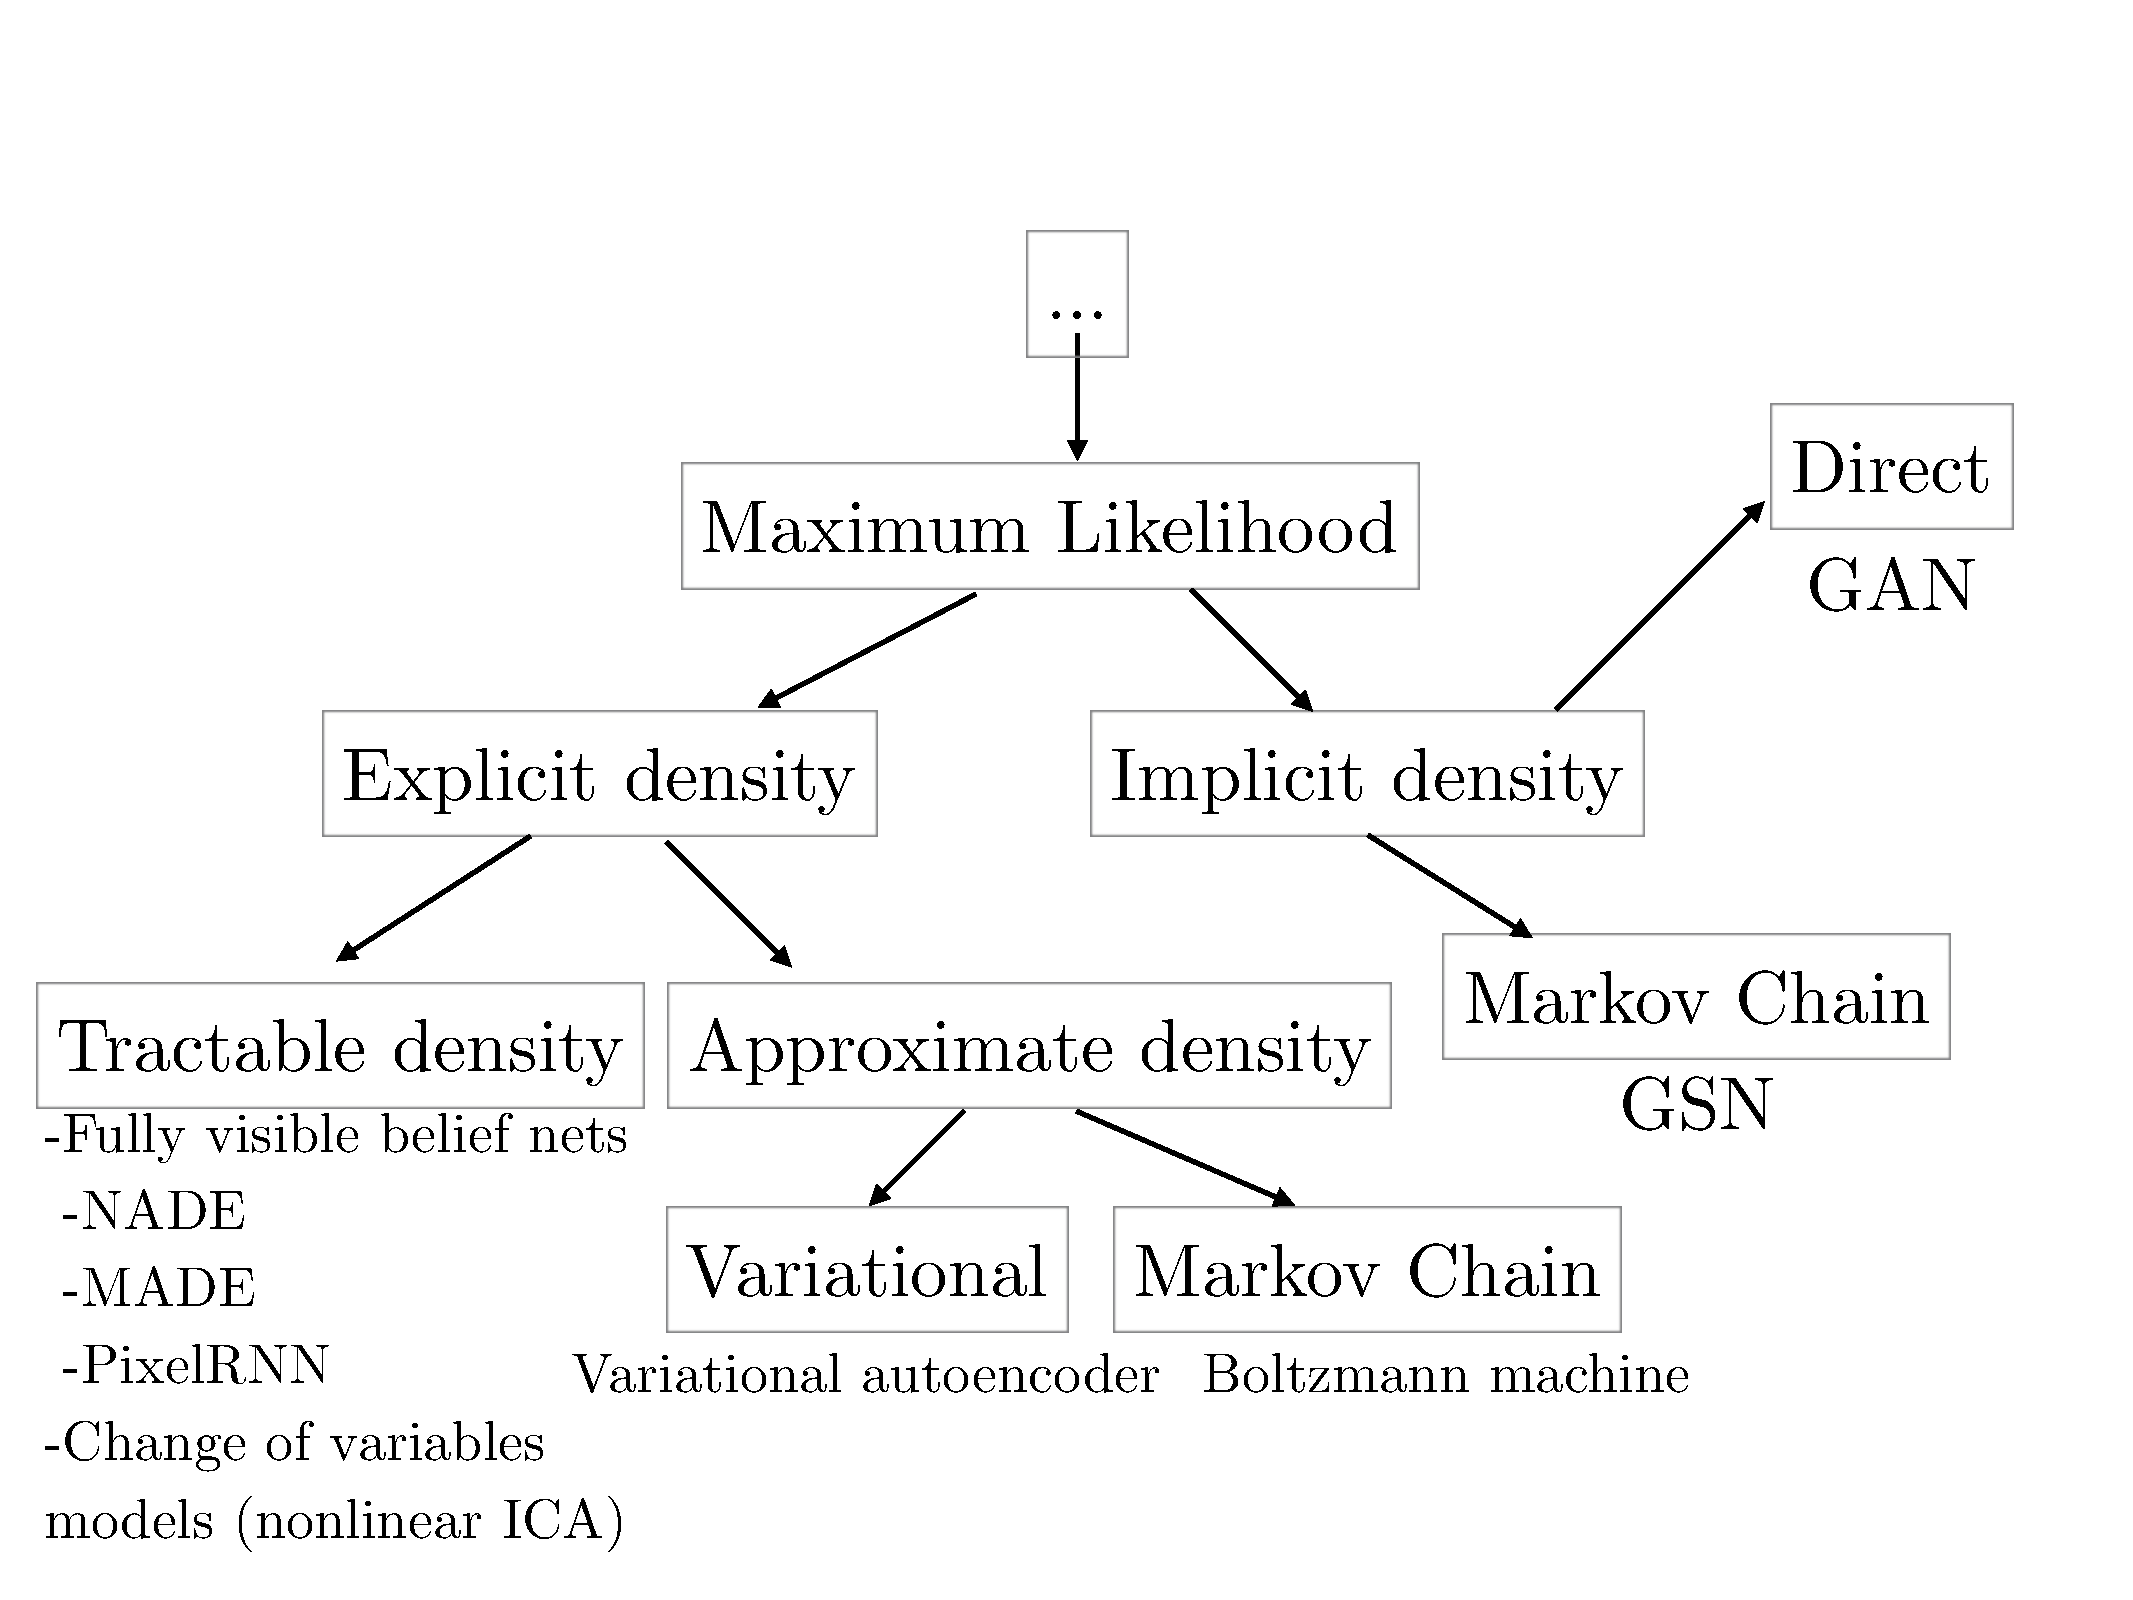
\includegraphics[width=\textwidth]{tree}
\caption{
Deep generative models that can learn via the principle of maximim likelihood
differ with respect to how they represent or approximate the likelihood.
On the left branch of this taxonomic tree, models construct an explicit density,
$\pmodel(\vx; \vtheta)$, and thus an explicit likelihood which can be maximized.
Among these explicit density models, the density may be computationally tractable,
or it may be intractable, meaning that to maximize the likelihood it is necessary
to make either variatioanl approximations or Monte
Carlo approximations (or both).
On the right branch of the tree, the model does not explicitly represent a
probability distribution over the space where the data lies.
Instead, the model provides some way of interacting less directly with this
probability distribution.
Typically the indirect means of interacting with the probability distribution is
the ability to draw samples from it.
Some of these implicit models that offer the ability to sample from the distribution
do so using a Markov Chain; the model defines a way to stochastically transform
an existing sample in order to obtain another sample from the same distribution.
Others are able to generate a sample in a single step, starting without any input.
While the models used for GANs can sometimes be constructed to define an explicit
density, the training algorithm for GANs makes use only of the model's ability to
generate samples.
GANs are thus trained using the strategy from the rightmost leaf of the tree:
using an implicit model that samples directly from the distribution represented
by the model.
}
\label{fig:tree}
\end{figure}

\subsection{Explicit density models}

In the left branch of the taxonomy shown in \figref{fig:tree} are models that define
an explicit density function $\pmodel(\vx ; \vtheta)$.
For these models, maxmimization of the likelihood is straightforward; we simply plug
the model's definition of the density function into the expression for the likelihood,
and follow the gradient uphill.

The main difficulty present in explicit density models is designing a model that can
capture all of the complexity of the data to be generated 
while still maintaining computational tractability.
There are two different strategies used to confront this challenge:
(1) careful construction of models whose structure guarantees their tractability,
as described in \secref{sec:explicit_tractable},
and (2) models that admit tractable approximations to the likelihood and its
gradients, as described in \secref{sec:approx}.

\subsubsection{Tractable explicit models}
\label{sec:explicit_tractable}

In the leftmost leaf of the taxonomic tree of \figref{fig:tree} are the models
that define an explicit density function that is computationally tractable.
There are currently two popular approaches to tractable explicit density models:
fully visible belief networks and nonlinear independent components analysis.

\paragraph{Fully visible belief networks}
\newterm{Fully visible belief networks} \citep{Frey96,Frey98} or FVBNs are models that use the chain
rule of probability to decompose a probability distribution over an $n$-dimensional vector $\vx$
into a product of one-dimensional probability distributions:
\[
\pmodel(\vx) = \prod_{i=1}^n \pmodel\left(\evx_i \mid \evx_1, \dots, \evx_{i-1} \right).
\]
FVBNs are, as of this writing, one of the three most popular
approaches to generative modeling, alongside GANs and variational autoencoders.
They form the basis for sophisticated generative models from DeepMind, such as
WaveNet \citep{aaron-wavenet-2016}. WaveNet is able to generate realistic human speech.
The main drawback of FVBNs is that samples must be generated
one entry at a time: first $\evx_1$, then $\evx_2$, etc., so the cost of generating
a sample is $O(n)$.
In modern FVBNs such as WaveNet, the distribution over each $\evx_i$ is computed by a deep
neural network, so each of these $n$ steps involves a nontrivial amount of computation.
Moreover, these steps cannot be parallelized.
WaveNet thus requires two minutes of computation time to generate one second of audio,
and cannot yet be used for interactive conversations.
GANs were designed to be able to generate all of $\vx$ in parallel, yielding greater
generation speed.

\paragraph{Nonlinear independent components analysis}
Another family of deep generative models with explicit density functions is based on
defining continuous, nonlinear transformations between two different spaces.
For example, if there is a vector of latent variables $\vz$ and a continuous, differentiable,
invertible transformation
$g$ such that $g(\vz)$ yields a sample from the model in $\vx$ space,
then
\begin{equation}
  \label{eq:change-of-variable}
  p_x(\vx) = p_z(g^{-1}(\vx)) \left| \mathrm{det}
  \left( \frac{\partial g^{-1}(\vx)} {\partial \vx}\right) \right|. 
\end{equation}
The density $p_x$ is tractable if the density $p_z$ is tractable
and the determinant of the Jacobian of $g^{-1}$ is tractable.
In other words, a simple distribution over $\vz$ combined with
a transformation $g$ that warps space in complicated ways can yield
a complicated distribution over $\vx$, and if $g$ is carefully designed,
the density is tractable too.
Models with nonlinear $g$ functions date back at least to
~\citet{hyvarinen1999nonlinear}.
The latest member of this family is real NVP \citep{dinh2016density}.
See \figref{fig:nvp} for some visualizations of ImageNet samples
generated by real NVP.
The main drawback to nonlinear ICA models is that they impose restrictions
on the choice of the function $g$. In particular, the invertibility requirement
means that the latent variables $\vz$ must have the same dimensionality as $\vx$.
GANs were designed to impose very few requirements on $g$, and, in particular,
admit the use of $\vz$ with larger dimension than $\vx$.

\begin{figure}
\centering
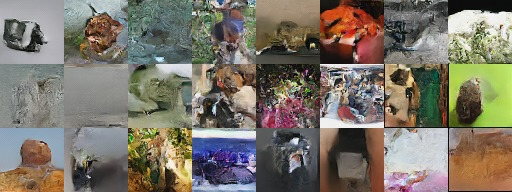
\includegraphics[width=\textwidth]{fig_imnet_64_samples}
\caption{Samples generated by a real NVP model trained on 64x64 ImageNet images.
Figure reproduced from \citet{dinh2016density}.}
\label{fig:nvp}
\end{figure}

For more information about the chain rule of probability used to define FVBNs
or about the effect of deterministic transformations on probability densities
as used to define nonlinear ICA models, see chapter 3 of \citet{Goodfellow-et-al-2016}.

In summary, models that define an explicit, tractable density are highly
effective, because they permit the use of an optimization algorithm directly
on the log-likelihood of the training data.
However, the family of models that provide a tractable density is limited,
with different families having different disadvantages.

\subsubsection{Explicit models requiring approximation}
\label{sec:approx}

To avoid some of the disadvantages imposed by the design requirements of models
with tractable density functions, other models have been developed that still
provide an explicit density function but use one that is intractable, requiring
the use of approximations to maximize the likelihood.
These fall roughly into two categories: those using deterministic approximations,
which almost always means variational methods, and those using stochastic approximations,
meaning Markov chain Monte Carlo methods.

\paragraph{Variational approximations}
Variational methods define a lower bound
\[ \mathcal{L}(\vx; \vtheta) \leq \log \pmodel(\vx; \vtheta). \]
A learning algorithm that maximizes $\mathcal{L}$ is guaranteed to obtain at least
as high a value of the log-likelihood as it does of $\mathcal{L}$.
For many families of models, it is possible to define an $\mathcal{L}$ that is computationally
tractable even when the log-likelihood is not.
Currently, the most popular approach to variational learning in deep generative models
is the \newterm{variational autoencoder} \citep{Kingma-arxiv2013,Rezende-et-al-ICML2014} or VAE.
Variational autoencoders are one of the three approaches to deep generative modeling that are
the most popular as of this writing, along with FVBNs and GANs.
The main drawback of variational methods is that the deterministic approximation induces some bias,
in the sense that even with a perfect optimization algorithm and infinite training data, the gap
between $\mathcal{L}$ and the true likelihood can result in $\pmodel$ learning something other than
the true $\pdata$.
GANs were designed to be unbiased, in the sense that with a large enough model and infinite data,
the Nash equilibrium for a GAN game corresponds to recovering $\pdata$ exactly.
In practice, variational methods often obtain very good likelihood, but are regarded as producing
lower quality samples.
There is not a good method of quantitatively measuring sample quality, so this is a subjective opinion,
not an empirical fact.
See \figref{fig:vae_samples} for an example of some samples drawn from a VAE.
While it is difficult to point to a single aspect of GAN design and say that it results in
better sample quality, GANs are generally regarded as producing better samples.
For more information about variational approximations, see chapter 19 of
\citet{Goodfellow-et-al-2016}.

\begin{figure}
  \centering
  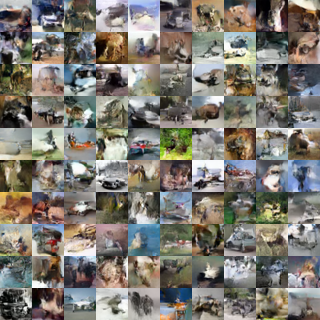
\includegraphics[width=\textwidth]{cifar_vae}
  \caption{Samples drawn from a VAE trained on the CIFAR-10 dataset.
    Figure reproduced from \citet{kingma2016improving}.
  }
  \label{fig:vae_samples}
\end{figure}

\paragraph{Markov chain approximations}
Most deep learning algorithms make use of some form of stochastic approximation,
at the very least in the form of using a small number of randomly selected training
examples to form a minibatch used to minimize the expected loss.
Usually, sampling-based approximations work reasonably well as long as a fair sample
can be generated quickly (e.g. selecting a single example from the training set
is a cheap operation) and as long as the variance across samples is not too high.
Some models require the generation of more expensive samples, using Markov chain
techniques.
A Markov chain is a process for generating samples by repeatedly drawing a sample
$\vx' \sim q(\vx' \mid \vx).$
By repeatedly updating $\vx$ according to the transition operator $q$, Markov chain
methods can sometimes guarantee that $\vx$ will eventually converge to a sample from
$\pmodel(\vx)$.
Unfortunately, this convergence can be very slow, and there is no clear way to test
whether the chain has converged, so in practice one often uses $\vx$ too early, before
it has truly converged to be a fair sample from $\pmodel$.
In high-dimensional spaces, Markov chains become less efficient.
Boltzmann machines \citep{Fahlman83,Ackley85,Hinton-Boltzmann,Hinton86a} are a
family of generative models that rely on Markov chains both to train the model
or to generate a sample from the model.
Boltzmann machines were an important part of the deep learning renaissance beginning
in 2006 \citep{Hinton06,hinton2007learning} but they are now used only very rarely,
presumably mostly because the underlying Markov chain approximation techniques have
not scaled to problems like ImageNet generation.
Moreover, even if Markov chain methods scaled well enough to be used for training,
the use of a Markov chain to generate samples from a trained model is undesirable
compared to single-step generation methods because the multi-step Markov chain
approach has higher computational cost.
GANs were designed to avoid using Markov chains for these reasons.
For more information about Markov chain Monte Carlo approximations, see chapter 18 of
\citet{Goodfellow-et-al-2016}.
For more information about Boltzmann machines, see chapter 20 of the same book.

Some models use both variational and Markov chain approximations.
For example, deep Boltzmann machines make use of both types of
approximation \citep{SalHinton09}.

\subsection{Implicit density models}

Some models can be trained without even needing to explicitly define a density
functions.
These models instead offer a way to train the model while interacting only
indirectly with $\pmodel$, usually by sampling from it.
These constitute the second branch, on the right side, of our taxonomy of
generative models depicted in \figref{fig:tree}.

Some of these implicit models based on drawing samples from $\pmodel$ define
a Markov chain transition operator that must be run several times to obtain
 a sample from the model.
From this family, the primary example is the \newterm{generative stochastic network}
\citep{Bengio-et-al-ICML-2014}.
As discussed in \secref{sec:approx}, Markov chains often fail to scale to high
dimensional spaces, and impose increased computational costs for using the
generative model. GANs were designed to avoid these problems.

Finally, the rightmost leaf of our taxonomic tree is the family of implicit models
that can generate a sample in a single step.
At the time of their introduction, GANs were the only notable member of this family,
but since then they have been joined by additional models based on
kernelized moment matching \citep{Li-et-al-2015,dziugaite2015training}.

\subsection{Comparing GANs to other generative models}

In summary, GANs were designed to avoid many disadvantages associated with other generative
models:
\begin{itemize}
  \item They can generate samples in parallel, instead of using runtime proportional to the
    dimensionality of $\vx$. This is an advantage relative to FVBNs.
  \item The design of the generator function has very few restrictions. This is an advantage
    relative to Boltzmann machines, for which few probability distributions admit tractable
    Markov chain sampling, and relative to nonlinear ICA, for which the generator must be
    invertible and the latent code $\vz$ must have the same dimension as the samples
    $\vx$.
  \item No Markov chains are needed. This is an advantage relative to Boltzmann machines and GSNs.
  \item No variational bound is needed, and thus the GAN framework is able to be asymptotically
    consistent. This is an advantage relative to VAEs.
  \item GANs are subjectively regarded as producing better samples than other methods.
\end{itemize}
At the same time, GANs have taken on a new disadvantage: training them requires finding
the Nash equilibrium of a game, which is a more difficult problem than optimizing an
objective function.

\section{How do GANs work?}

We have now seen several other generative models and explained that GANs do not
work in the same way that they do. But how do GANs themselves work?

\subsection{The GAN framework}

The basic idea of GANs is to set up a game between two players.
One of them is called the \newterm{generator}.
The generator creates samples that are intended to come from the
same distribution as the training data.
The other player is the \newterm{discriminator}.
The discriminator examines samples to determine whether they are real
or fake.
The discriminator learns using traditional supervised learning techniques,
dividing inputs into two classes (real or fake).
The generator is trained to fool the discriminator.
We can think of the generator as being like a counterfeiter, trying to
make fake money, and the discriminator as being like police, trying to
allow legitimate money and catch counterfeit money.
To succeed in this game, the counterfeiter must learn to make money that
is indistinguishable from genuine money, and the generator network must
learn to create samples that are drawn from the same distribution as the
training data.
The process is illustrated in \figref{fig:framework}.

\begin{figure}
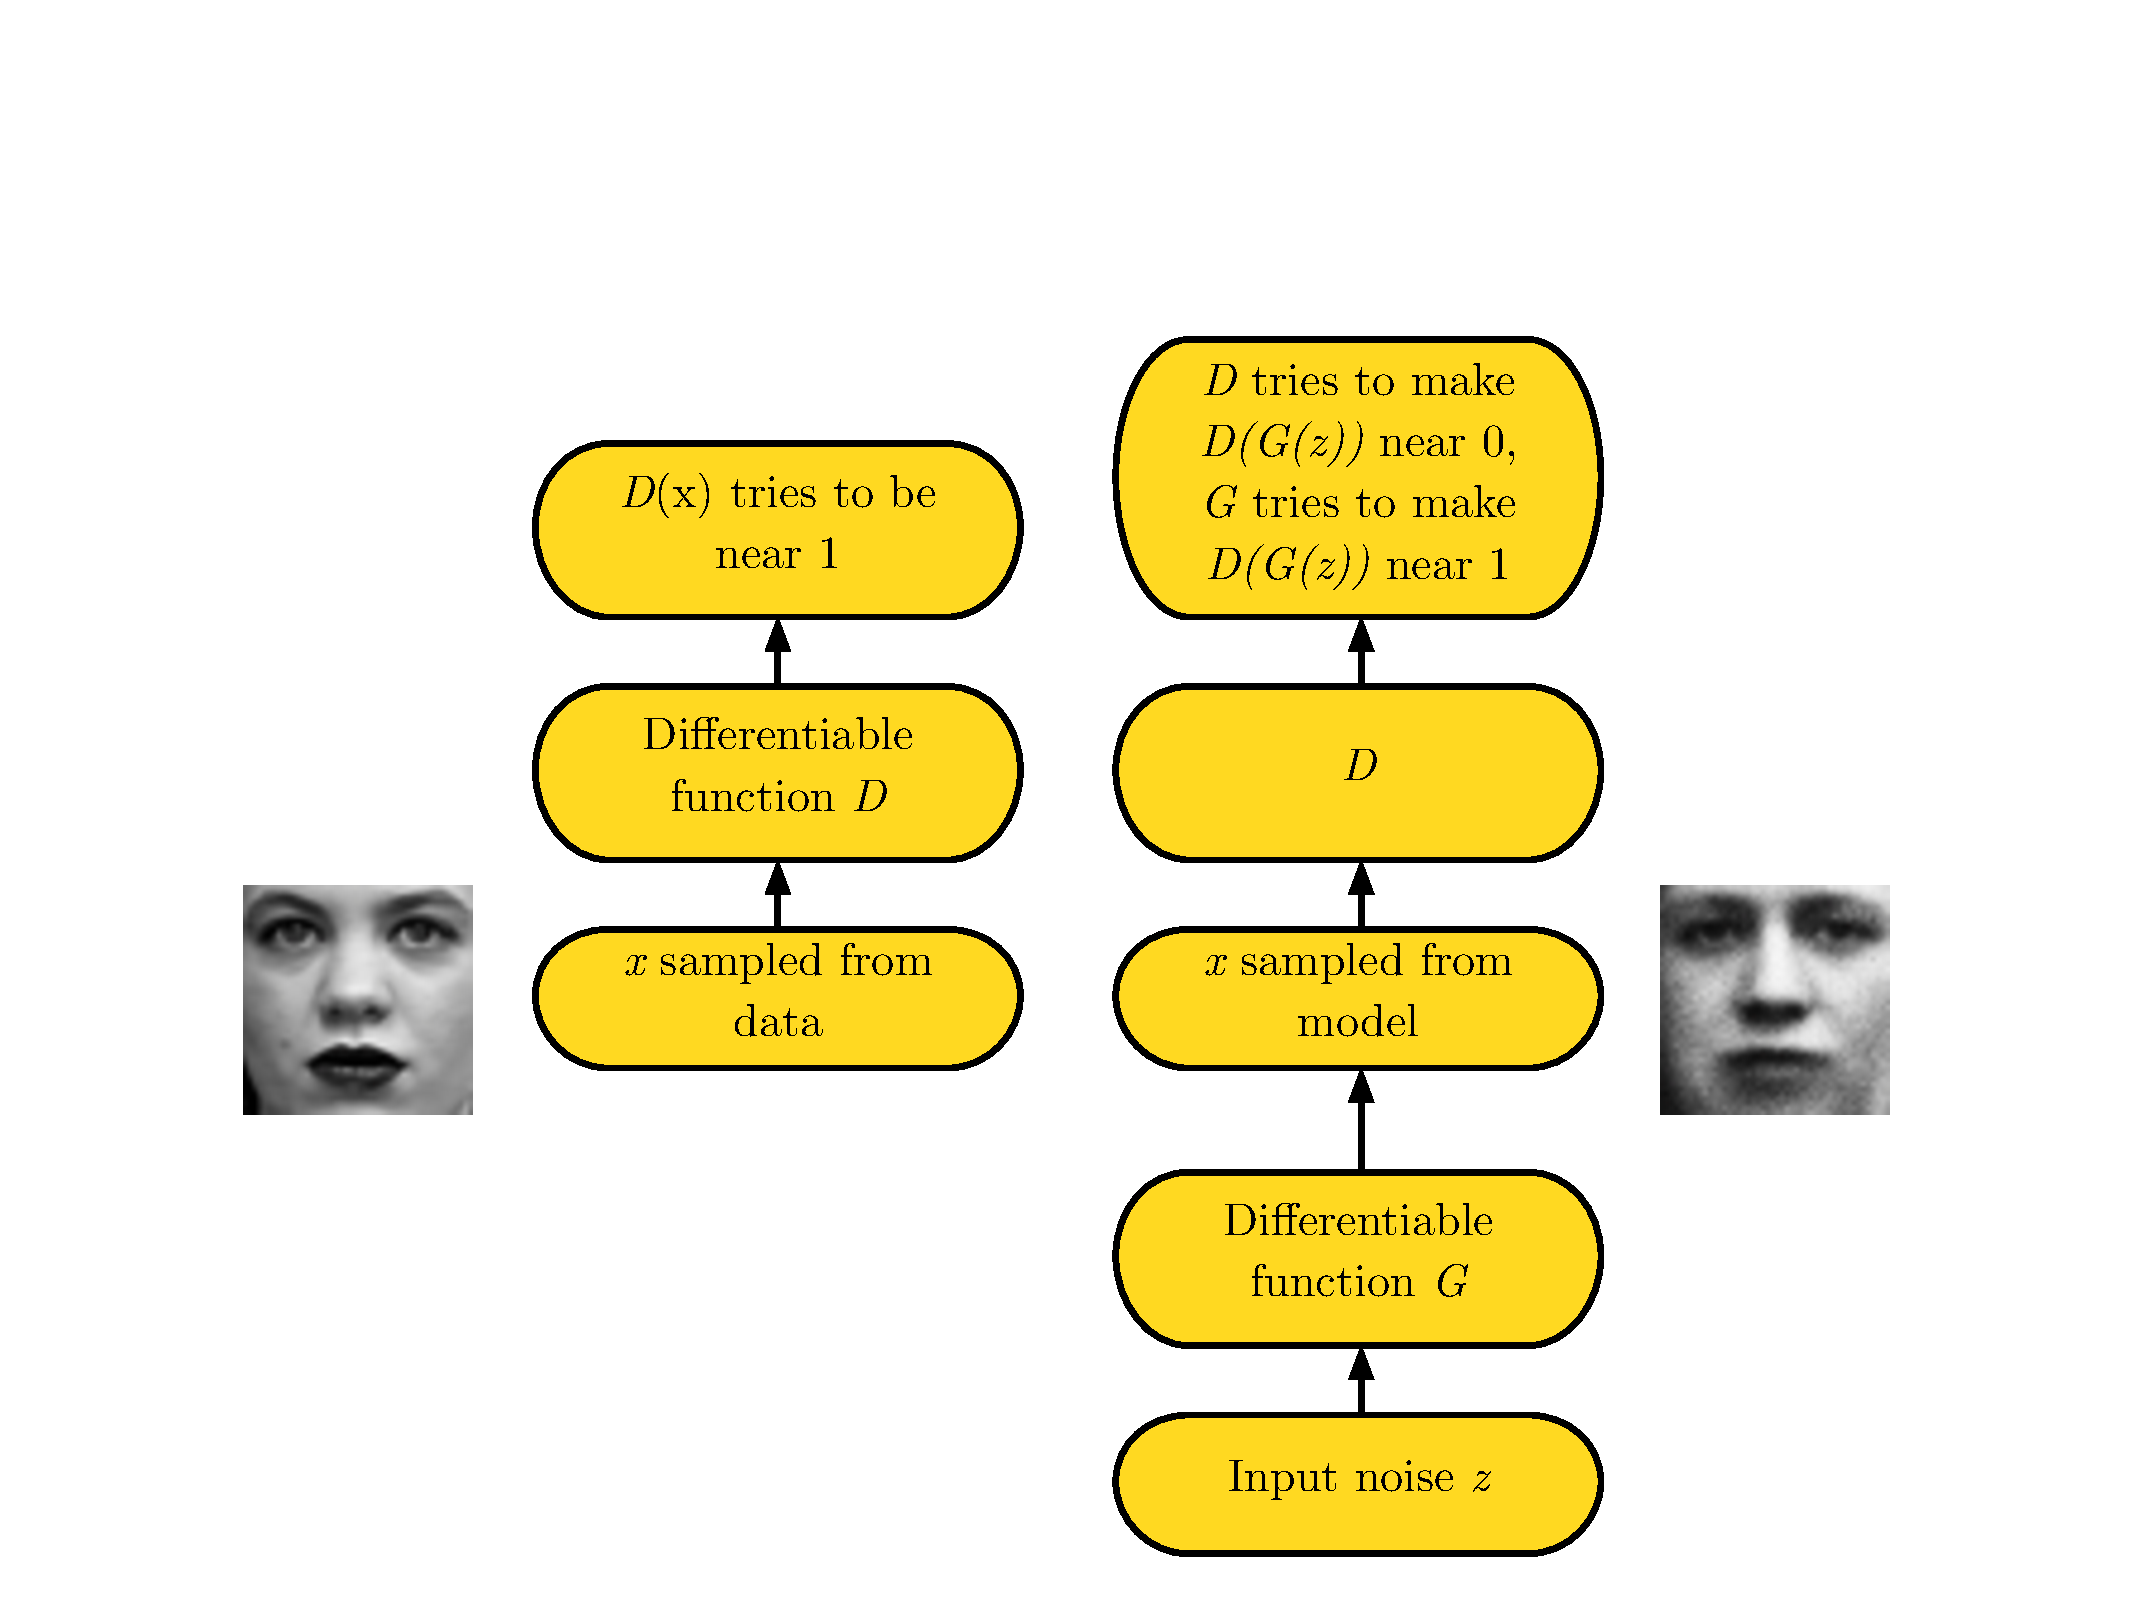
\includegraphics[width=\textwidth]{framework}
\caption{The GAN framework pits two adversaries against each other in a game.
Each player is represented by a differentiable function controlled by a set
of parameters.
Typically these functions are implemented as deep neural networks.
The game plays out in two scenarios.
In one scenario, training examples $\vx$ are randomly sampled from the training
set and used as input for the first player, the discriminator, represented
by the function $D$. The goal of the discriminator is to output the probability
that its input is real rather than fake, under the assumption that half of the
inputs it is ever shown are real and half are fake.
In this first scenario, the goal of the discriminator is for $D(\vx)$ to be
near 1.
In the second scenario, inputs $\vz$ to the generator are randomly sampled from
the model's prior over the latent variables.
The discriminator then receives input $G(\vz)$, a fake sample created by the
generator.
In this scenario, both players participate. The discriminator strives to make
$D(G(z))$ approach 0 while the generative strives to make the same quantity
approach 1.
If both models have sufficient capacity, then the Nash equilibrium of this game
corresponds to the $G(\vz)$ being drawn from the same distribution as the training
data, and $D(\vx) = \frac{1}{2}$ for all $\vx$.
}
\label{fig:framework}
\end{figure}

Formally, GANs are a structured probabilistic model (see chapter 16 of
\citet{Goodfellow-et-al-2016} for an introduction to structured probabilistic
models) containing latent variables $\vz$ and observed variables $\vx$.
The graph structure is shown in \figref{fig:graph}.

The two players in the game are represented by two functions, each of which
is differentiable both with respect to its inputs and with respect to its
parameters.
The discriminator is a function $D$ that takes $\vx$ as input and uses
$\vtheta^{(D)}$ as parameters.
The generator is defined by a function $G$ that takes $\vz$ as input and
uses $\vtheta^{(G)}$ as parameters.

Both players have cost functions that are defined in terms of both players'
parameters.
The discriminator wishes to minimize $J^{(D)}\left( \vtheta^{(D)}, \vtheta^{(G)} \right)$
and must do so while controlling only $\vtheta^{(D)}$.
The generator wishes to minimize $J^{(G)}\left( \vtheta^{(D)}, \vtheta^{(G)} \right)$
and must do so while controlling only $\vtheta^{(G)}$.
Because each player's cost depends on the other player's parameters, but each player
cannot control the other player's parameters, this scenario is most
straightforward to describe as a game rather than as an optimization problem.
The solution to an optimization problem is a (local) minimum, a point in parameter space
where all neighboring points have greater or equal cost.
The solution to a game is a Nash equilibrium.
Here, we use the terminology of local differential Nash equilibria \citep{ratliff2013characterization}.
In this context, a Nash equilibrium is a tuple $(\vtheta^{(D)}, \vtheta^{(G)} )$
that is a local minimum of $J^{(D)}$ with respect to $\vtheta^{(D)}$ and a local
minimum of $J^{(G)}$ with respect to $\vtheta^{(G)}$.

\paragraph{The generator}
The generator is simply a differentiable function $G$.
When $\vz$ is sampled from some simple prior distribution,
$G(\vz)$ yields a sample of $\vx$ drawn from $\pmodel$.
Typically, a deep neural network is used to represent $G$.
Note that the inputs to the function $G$ do not need to correspond
to inputs to the first layer of the deep neural net; inputs may
be provided at any point throughout the network.
For example, we can partition $\vz$ into two vectors $\vz^{(1)}$
and $\vz^{(2)}$, then feed $\vz^{(1)}$ as input to the first layer
of the neural net and add $\vz^{(2)}$ to the last layer of the neural
net. If $\vz^{(2)}$ is Gaussian, this makes $\vx$ conditionally Gaussian
given $\vz^{(1)}$.
Another popular strategy is to apply additive or multiplicative noise to
hidden layers or concatenate noise to hidden layers of the neural net.
Overall, we see that there are very few restrictions on the design of
the generator net.
If we want $\pmodel$ to have full support on $\vx$ space we need the dimension
of $\vz$ to be at least as large as the dimension of $\vx$, and $G$ must be
differentiable, but those are the only requirements.
In particular, note that any model that can be trained with the nonlinear
ICA approach can be a GAN generator network.
The relationship with variational autoencoders is more complicated;
the GAN framework can train some models that the VAE framework cannot and vice
versa, but the two frameworks also have a large intersection.
The most salient difference is that, if relying on standard backprop,
VAEs cannot have discrete variables at the input to the generator,
while GANs cannot have discrete variables at the output of the generator.

\paragraph{The training process}
The training process consists of simultaneous SGD.
On each step, two minibatches are sampled: a minibatch of $\vx$ values from
the dataset and a minibatch of $\vz$ values drawn from the model's prior over
latent variables.
Then two gradient steps are made simultaneously:
one updating $\vtheta^{(D)}$ to reduce $J^{(D)}$
and one updating $\vtheta^{(G)}$ to reduce $J^{(G)}$.
In both cases, it is possible to use the gradient-based optimization algorithm
of your choice.
Adam \citep{kingma2014adam} is usually a good choice.
Many authors recommend running more steps of one player than the other, but
as of late 2016, the author's opinion is that the protocol that works the best
in practice is simultaneous gradient descent, with one step for each player.


\begin{figure}
  \centering
  
\includegraphics{graph}
  \caption{The graphical model structure of GANs, which is also shared with
    VAEs, sparse coding, etc.
    It is directed graphical model where every latent variable influences
    every observed variable.
    Some GAN variants remove some of these connections.
  }
  \label{fig:graph}
\end{figure}

\subsection{Cost functions}

Several different cost functions may be used within the GANs framework.

\subsubsection{The discriminator's cost, $J^{(D)}$}

All of the different games designed for GANs so far use the same cost for the
discriminator, $J^{(D)}$. They differ only in terms of the cost used for the
generator, $J^{(G)}$.

The cost used for the discriminator is:
\begin{equation}
  J^{(D)}(\vtheta^{(D)}, \vtheta^{(G)}) = -\frac{1}{2} \E_{\vx \sim \pdata} \log D(\vx; \vtheta^{(D)}) - \frac{1}{2} \E_{\vz} \log \left(1 - D\left( G(z); \vtheta^{(G)} \right) \right).
  \label{eq:discriminator_cost}
\end{equation}

This is just the standard cross-entropy cost that is minimized when training a standard binary classifier
with a sigmoid output.
The only difference is that the classifier is trained on two minibatches of data; one coming from the
dataset, where the label is $1$ for all examples, and one coming from the generator, where the label
is $0$ for all examples.


\subsubsection{Minimax}

So far we have specified the cost function for only the discriminator.
A complete specification of the game requires that we specify a cost function also
for the generator.

The simplest version of the game is a \newterm{zero-sum game}, in which the sum of all player's
costs is always zero.
In this version of the game,
\[ J^{(G)} = - J^{(D)} .\]

Because $J^{(G)}$ is tied directly to $J^{(D)}$, we can summarize the entire game with a
\newterm{value function} specifying the discriminator's payoff:
\[ V\left(\vtheta^{(D)}, \vtheta^{(G)} \right) = - J^{(D)} \left(\vtheta^{(D)}, \vtheta^{(G)} \right).\]

Zero-sum games are also called \newterm{minimax} games because their solution involves minimization
in an outer loop and maximization in an inner loop:
\[ \vtheta^{(G)*} = \argmin_{\vtheta^{(G)}} \max_{\vtheta^{(D)}} V\left(\vtheta^{(D)}, \vtheta^{(G)} \right) . \]

The minimax game is mostly of interest because it is easily amenable to theoretical analysis.
\citet{Goodfellow-et-al-NIPS2014-small} used this variant of the GAN game to show that learning in
this game resembles minimizing the Jensen-Shannon divergence between the data and the model distribution,
and that the game converges to its equilibrium if both players' policies can be updated directly in
function space.
In practice, the players are represented with deep neural nets and updates are made in parameter space,
so these results, which depend on convexity, do not apply.

\subsubsection{Heuristic, non-saturating game}

TODO

In the minimax game, the generator minimizes the log-probability of the discriminator being correct.
In this game, the generator maximizes the log-probability of the discriminator being mistaken.

\section{Tips and Tricks}

Practitioners use several tricks to improve the performance of GANs.
It can be difficult to tell how effective some of these tricks are;
many of them seem to help in some contexts and hurt in others.
These should be regarded as techniques that are worth trying out,
not as ironclad best practices.

NIPS 2016 also featured a workshop on adversarial training, with
an invited talk by Soumith Chintala called "How to train a GAN."
This talk has more or less the same goal as this portion of the tutorial,
with a different collection of advice.
To learn about tips and tricks not included in this tutorial, check
out the GitHub repository associated with Soumith's talk:

\url{https://github.com/soumith/ganhacks}


\subsection{Train with labels}

Using labels in any way, shape or form almost always results in a dramatic
improvement in the subjective quality of the samples generated by the model.
This was first observed by \citet{denton2015deep}, who built class-conditional
GANs that generated much better samples than GANs that were free to generate
from any class.
Later, \citet{salimans2016improved} found that sample quality improved
even if the generator did not explicitly incorporate class information; training
 the discriminator to recognize specific classes of real objects is sufficient.

 It is not entirely clear why this trick works.
 It may be that the incorporation of class information gives the training
 process useful clues that help with optimization.
 It may also be that this trick gives no objective improvement in sample quality,
 but instead biases the samples toward taking on properties that the human
 visual system focuses on.
 If the latter is the case, then this trick may not result in a better model
 of the true data-generating distribution, but it still helps to create media
 for a human audience to enjoy and may help an RL agent to carry out tasks
 that rely on knowledge of the same aspects of the environment that are relevant
 to human beings.

 It is important to compare results obtained using this trick only to other
 results using the same trick; models trained with labels should be compared
 only to other models trained with labels, class-conditional models should
 be compared only to other class-conditional models.
 Comparing a model that uses labels to one that does not is unfair and an
 uninteresting benchmark, much as a convolutional model can usually be expected
 to outperform a non-convolutional model on image tasks.

\subsection{One-sided label smoothing}
\label{sec:label_smooth}

GANs are intended to work when the discriminator estimates a ratio of two
densities, but deep neural nets are prone to producing highly confident
outputs that identify the correct class but with too extreme of a probability.
This is especially the case when the input to the deep network is adversarially
constructed; the classifier tends to linearly extrapolate and produce
extremely confident predictions \citep{Goodfellow-2015-adversarial}.

To encourage the discriminator to estimate soft probabilities rather than
to extrapolate to extremely confident classification, we can use a technique
called \newterm{one-sided label smoothing} \citep{salimans2016improved}.

Usually we train the discriminator using \eqref{eq:discriminator_cost}.
We can write this in TensorFlow \citep{tensorflow} code as:
\begin{lstlisting}
d_on_data = discriminator_logits(data_minibatch)
d_on_samples = discriminator_logits(samples_minibatch)
loss = tf.nn.sigmoid_cross_entropy_with_logits(d_on_data, 1.) + \
       tf.nn.sigmoid_cross_entropy_with_logits(d_on_samples, 0.)
\end{lstlisting}

The idea of one-sided label smoothing is to replace the target for the real examples
with a value slightly less than one, such as .9:

\begin{lstlisting}
loss = tf.nn.sigmoid_cross_entropy_with_logits(d_on_data, .9) + \
       tf.nn.sigmoid_cross_entropy_with_logits(d_on_samples, 0.)
\end{lstlisting}

This prevents extreme extrapolation behavior in the discriminator; if it learns
to predict extremely large logits corresponding to a probability approaching $1$
for some input, it will be penalized and encouraged to bring the logits back
down to a smaller value.

It is important to not smooth the labels for the fake samples.
Suppose we use a target of $1-\alpha$ for the real data and a target of $0+\beta$
for the fake samples.
Then the optimal discriminator function is
\[ D^*(\vx) = \frac{(1-\alpha) \pdata(\vx) + \beta \pmodel(\vx)} { \pdata(\vx) + \pmodel(\vx) }.\]

When $\beta$ is zero, then smoothing by $\alpha$ does nothing but scale down the optimal value
of the discriminator.
When $\beta$ is nonzero, the shape of the optimal discriminator function changes.
In particular, in a region where $\pdata(\vx)$ is very small and $\pmodel(\vx)$ is larger,
$D^*(\vx)$ will have a peak near the spurious mode of $\pmodel(\vx)$.
The discriminator will thus reinforce incorrect behavior in the generator; the generator
will be trained either to produce samples that resemble the data or to produce samples
that resemble the samples it already makes.

One-sided label smoothing is a simple modification of the much older label smoothing
technique, which dates back to at least the 1980s.
\citet{Szegedy-et-al-2015} demonstrated that label smoothing is an excellent regularizer
in the context of convolutional networks for object recognition.
One reason that label smoothing works so well as a regularizer is that it does not
ever encourage the model to choose an incorrect class on the training set, but only
to reduce the confidence in the correct class.
Other regularizers such as weight decay often encourage some misclassification
if the coefficient on the regularizer is set high enough.
\citet{wardefarley2016} showed that label smoothing can help to reduce vulnerability to
adversarial examples, which suggests that label smoothing should help the discriminator
more efficiently learn to resist attack by the generator.

\subsection{Virtual batch normalization}

Since the introduction of DCGANs, most GAN architectures have involved some form
of batch normalization.
The main purpose of batch normalization is to improve the optimization of the model,
by reparameterizing the model so that the mean and variance of each feature are determined
by a single mean parameter and a single variance parameter associated with that feature,
rather than by a complicated interaction between all of the weights of all of the layers
used to extract the feature.
This reparameterization is accomplished by subtracting the mean and dividing by the standard
deviation of that feature on a minibatch of data.
It is important that the normalization operation is {\em part of the model},
so that back-propgation computes the gradient of features that are defined to always
be normalized.
The method is much less effect if features are frequently renormalized after learning
without the normalization defined as part of the model.

Batch normalization is very helpful, but for GANs has a few unfortunate side effects.
The use of a different minibatch of data to compute the normalization statistics
on each step of training results in fluctuation of these normalizing constants.
When minibatch sizes are small (as is often the case when trying to fit a large generative
model into limited GPU memory) these fluctuations can become large enough that they
have more effect on the image generated by the GAN than the input $\vz$ has.
See \figref{fig:bad_batchnorm} for an example.

\begin{figure}
\centering
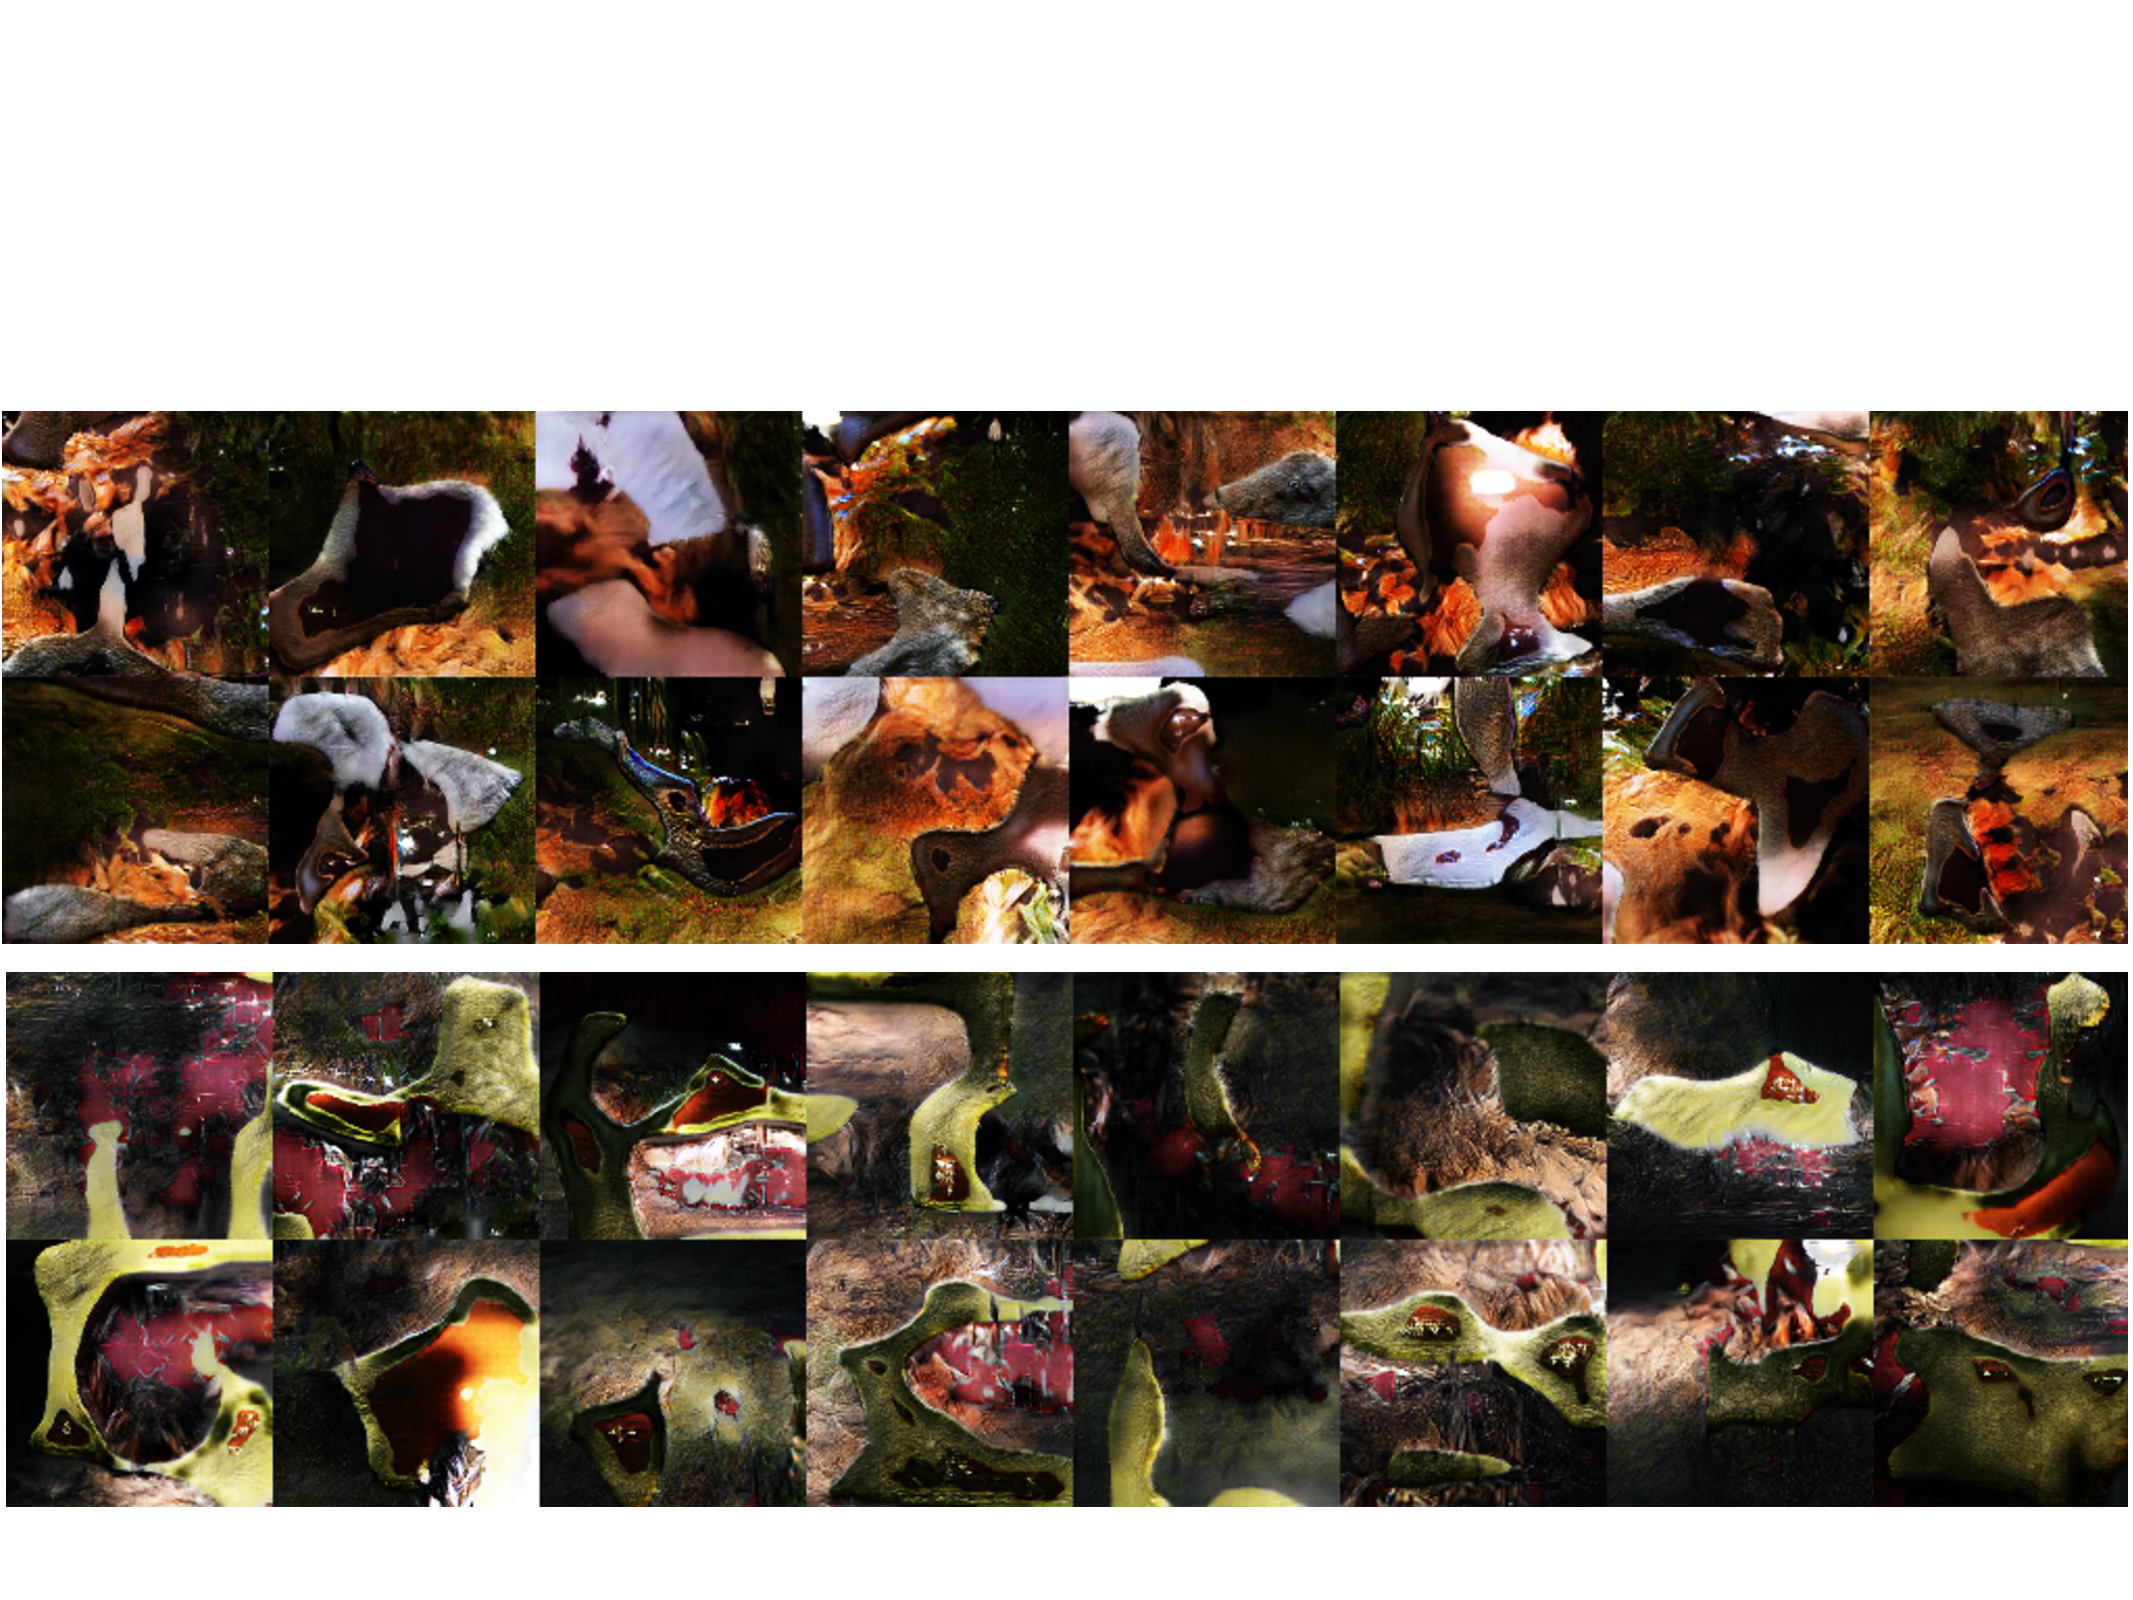
\includegraphics[width=\figwidth]{bad_batchnorm}
\caption{
Two minibatches of sixteen samples each, generated by a generator network using
batch normalization.
These minibatches illustrate a problem that occurs occasionally when using batch
normalization: fluctuations in the mean and standard deviation of feature values
in a minibatch can have a greater effect than the individual $\vz$ codes for individual
images within the minibatch.
This manifests here as one minibatch containing all orange-tinted samples and the other
containing all green-tinted samples.
The examples within a minibatch should be independent from each other, but in this
case, batch normalization has caused them to become correlated with each other.
}
\label{fig:bad_batchnorm}
\end{figure}

\citet{salimans2016improved} introduced techniques to mitigate this problem.
\newterm{Reference batch normalization} consists of running the network twice:
once on a minibatch of \newterm{reference examples} that are sampled once at the
start of training and never replaced, and once on the current minibatch of examples
to train on.
The mean and standard deviation of each feature are computed using the reference
batch. The features for both batches are then normalized using these computed statistics.
A drawback to reference batch normalization is that the model can overfit to the
reference batch. To mitigate this problem slightly, one can instead use
\newterm{virutal batch normalization}, in which the normalization statistics for each
example are computed using the union of that example and the reference batch.
Both reference batch normalization and virtual batch normalization have the property
that all examples in the training minibatch are processed independently from each other,
and all samples produced by the generator (except those defining the reference batch)
are i.i.d.

\subsection{Can one balance $G$ and $D$?}

Many people have an intuition that it is necessary to somehow balance the two players
to prevent one from overpowering the other.
If such balance is desirable and feasible, it has not yet been demonstrated in any
compelling fashion.

The author's present belief is that GANs work by estimating the ratio of the data density
and model density. This ratio is estimated correctly only when the discriminator is
optimal, so it is fine for the discriminator to overpower the generator.

Sometimes the gradient for the generator can vanish when the discriminator becomes
too accurate.
The right way to solve this problem is not to limit the power of the discriminator,
but to use a parameterization of the game where the gradient does not vanish
(\secref{sec:heuristic}).

Sometimes the gradient for the generator can become very large if the discriminator
becomes too confident. Rather than making the discriminator less accurate, a better
way to resolve this problem is to use one-sided label smoothing (\secref{sec:label_smooth}).

The idea that the discriminator should always be optimal in order to best estimate
the ratio would suggest training the discriminator for $k > 1$ steps every time
the generator is trained for one step. In practice, this does not usually result in a
clear improvement.

One can also try to balance the generator and discriminator by choosing the model
size.
In practice, the discriminator is usually deeper and sometimes has more filters
per layer than the generator.
This may be because it is important for the discriminator to be able to correctly
estimate the ratio between the data density and generator density, but it may
also be an artifact of the mode collapse problem---since the generator tends not
to use its full capacity with current training methods, practitioners presumably
do not see much of a benefit from increasing the generator capacity.
If the mode collapse problem can be overcome, generator sizes will presumably
increase. It is not clear whether discriminator sizes will increase proportionally.



\section{Research Frontiers}

GANs are a relatively new method, with many research directions still
remaining open.

\subsection{Non-convergence}

The largest problem facing GANs that researchers should try to resolve is the issue
of non-convergence.

Most deep models are trained using an optimization algorithm that seeks out a low
value of a cost function.
While many problems can interfere with optimization, optimization algorithms usually
make reliable downhill progress.
GANs require finding the equilibrium to a game with two players.
Even if each player successfully moves downhill on that player's update,
the same update might move the other player uphill.
Sometimes the two players eventually reach an equilibrium, but in other scenarios
they repeatedly undo each others' progress without arriving anywhere useful.
This is a general problem with games not unique to GANs, so a general solution
to this problem would have wide-reaching applications.



\section{Plug and Play Generative Networks}

Shortly before this tutorial was presented at NIPS, a new generative model
was released. This model, plug and play generative networks \citep{nguyen2016plug}, has dramatically
improved the diversity of samples of images of ImageNet classes that can be
produced at high resolution.

PPGNs are new and not yet well understood.
The model is complicated, and most of the recommendations about how to design the model
are based on empirical observation rather than theoretical understanding.
This tutorial will thus not say too much about exactly how PPGNs work, since this will
presumably become more clear in the future.

As a brief summary, PPGNs are basically an approximate Langevin sampling approach to
generating images with a Markov chain.
The gradients for the Langevin sampler are estimated using a denoising autoencoder.
The denoising autoencoder is trained with several losses, including a GAN loss.

Some of the results are shown in \figref{fig:ppgn}.
As demonstrated in \figref{fig:recons}, the GAN loss is crucial for obtaining high quality images.

\begin{figure}
\centering
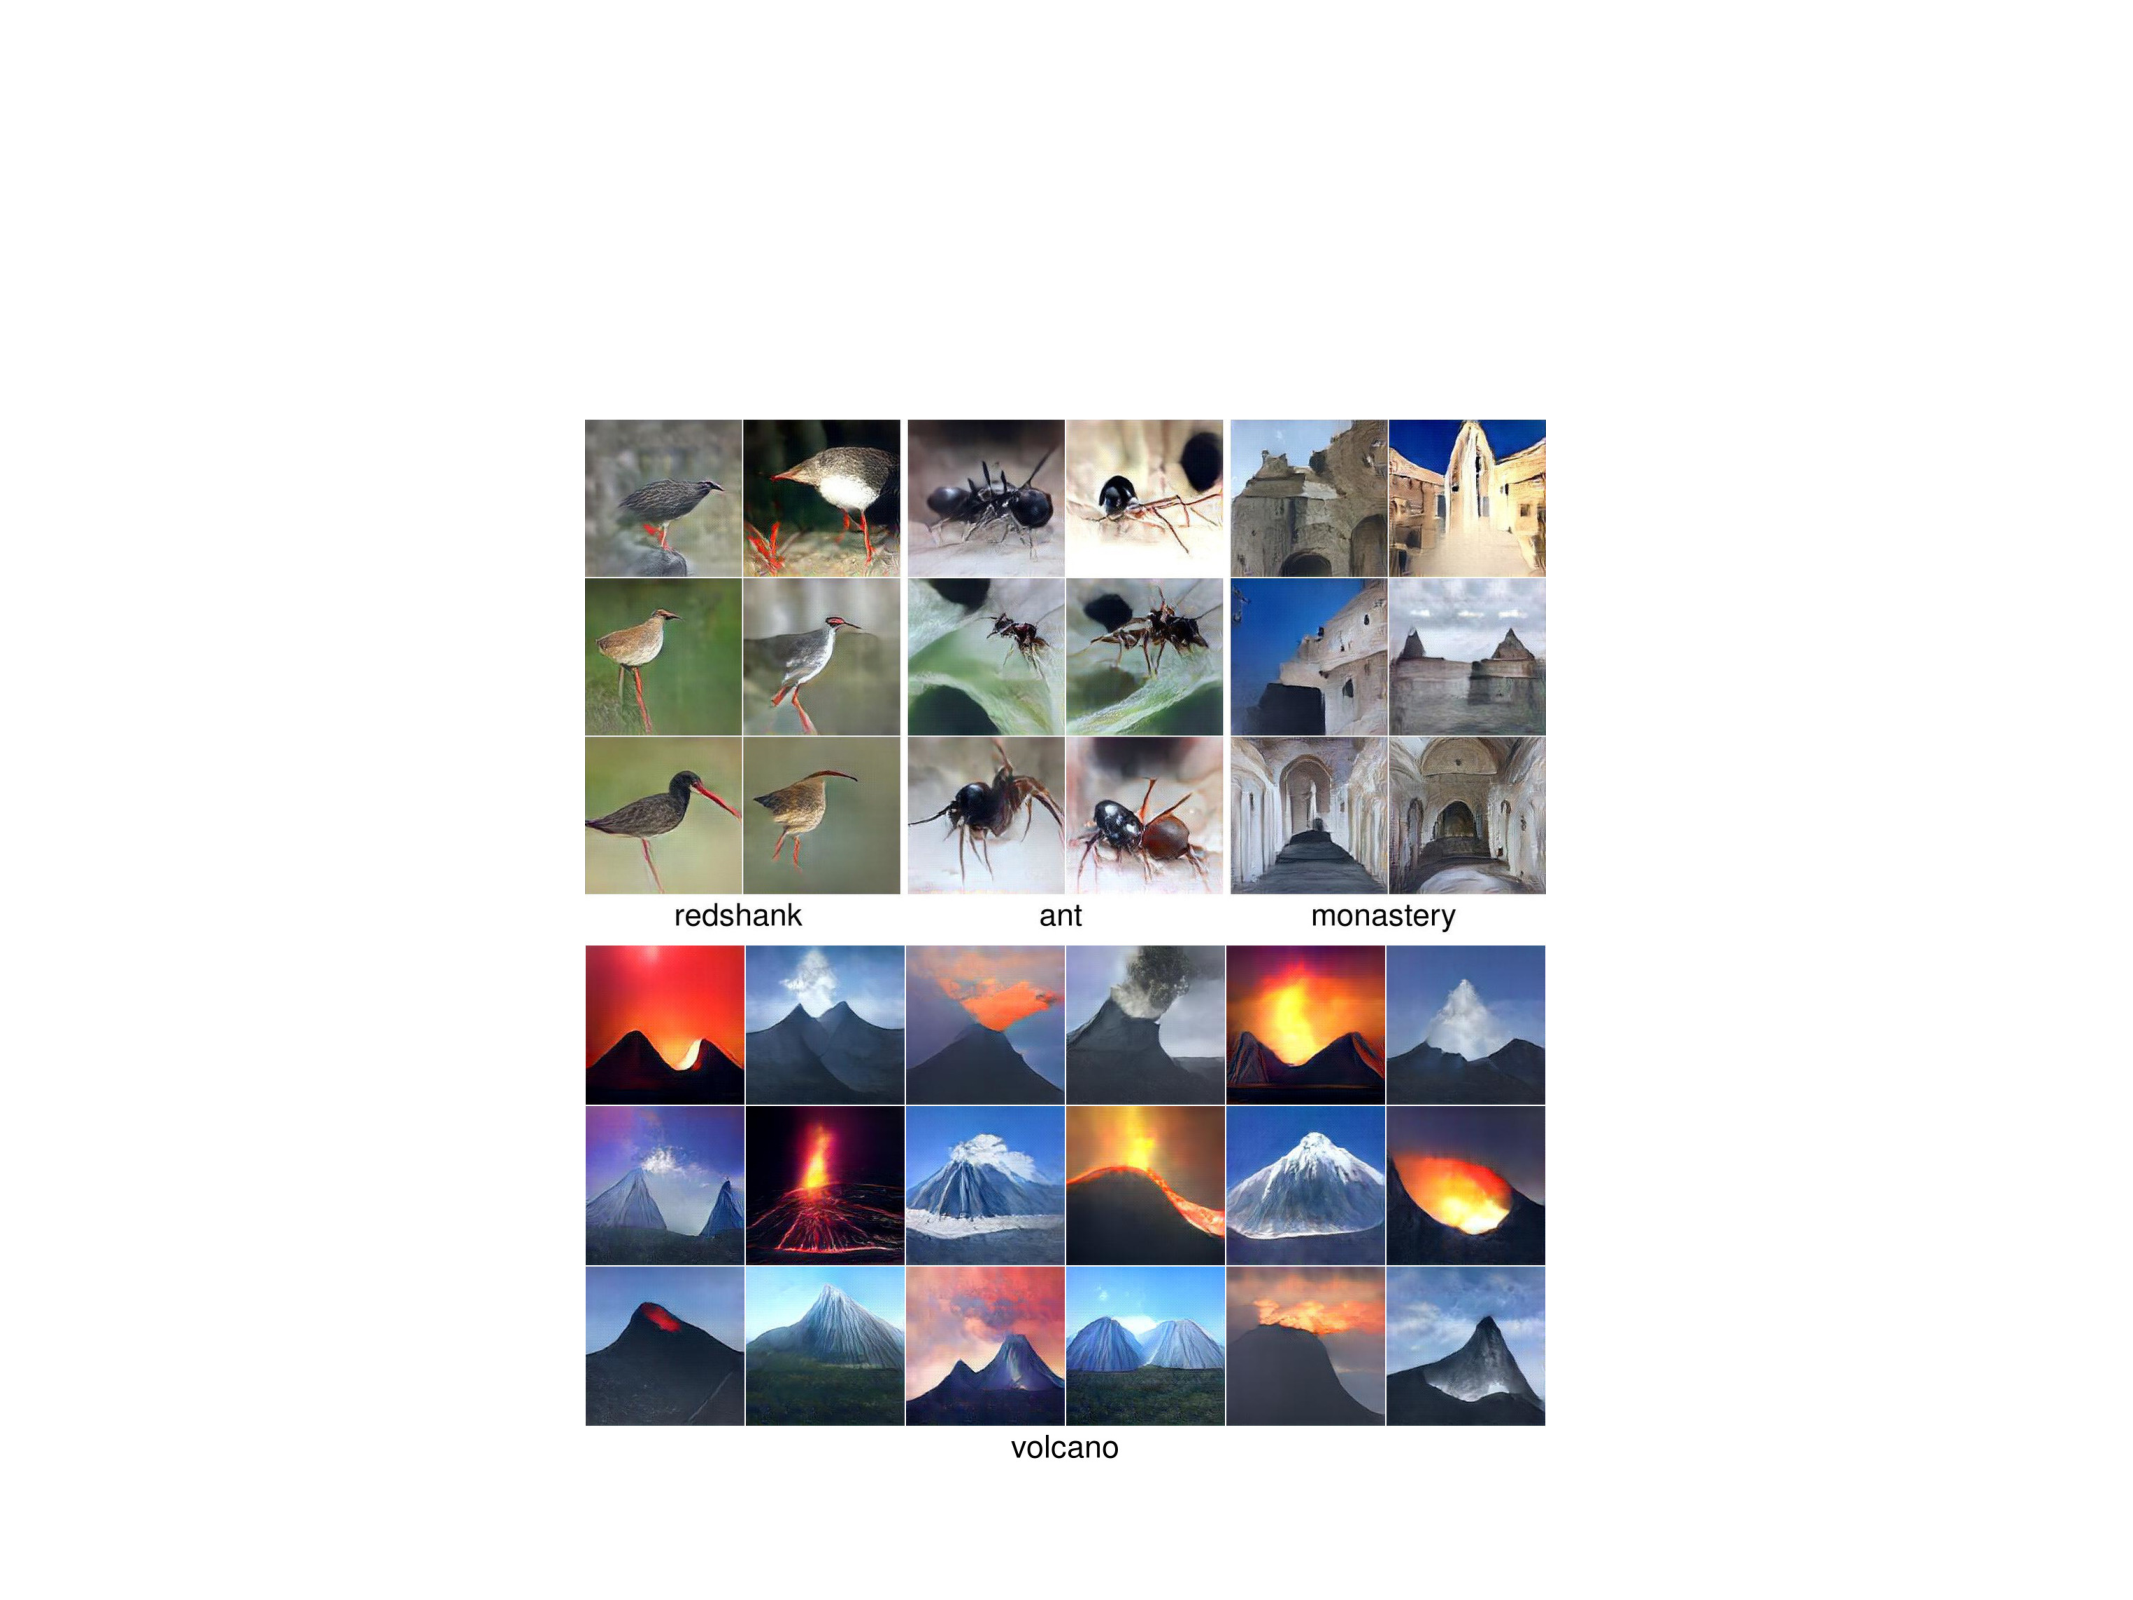
\includegraphics[width=\figwidth]{ppgn}
\caption{PPGNs are able to generate diverse, high resolution images from ImageNet
classes. Image reproduced from \citet{nguyen2016plug}.}
\label{fig:ppgn}
\end{figure}


\begin{figure}
\centering
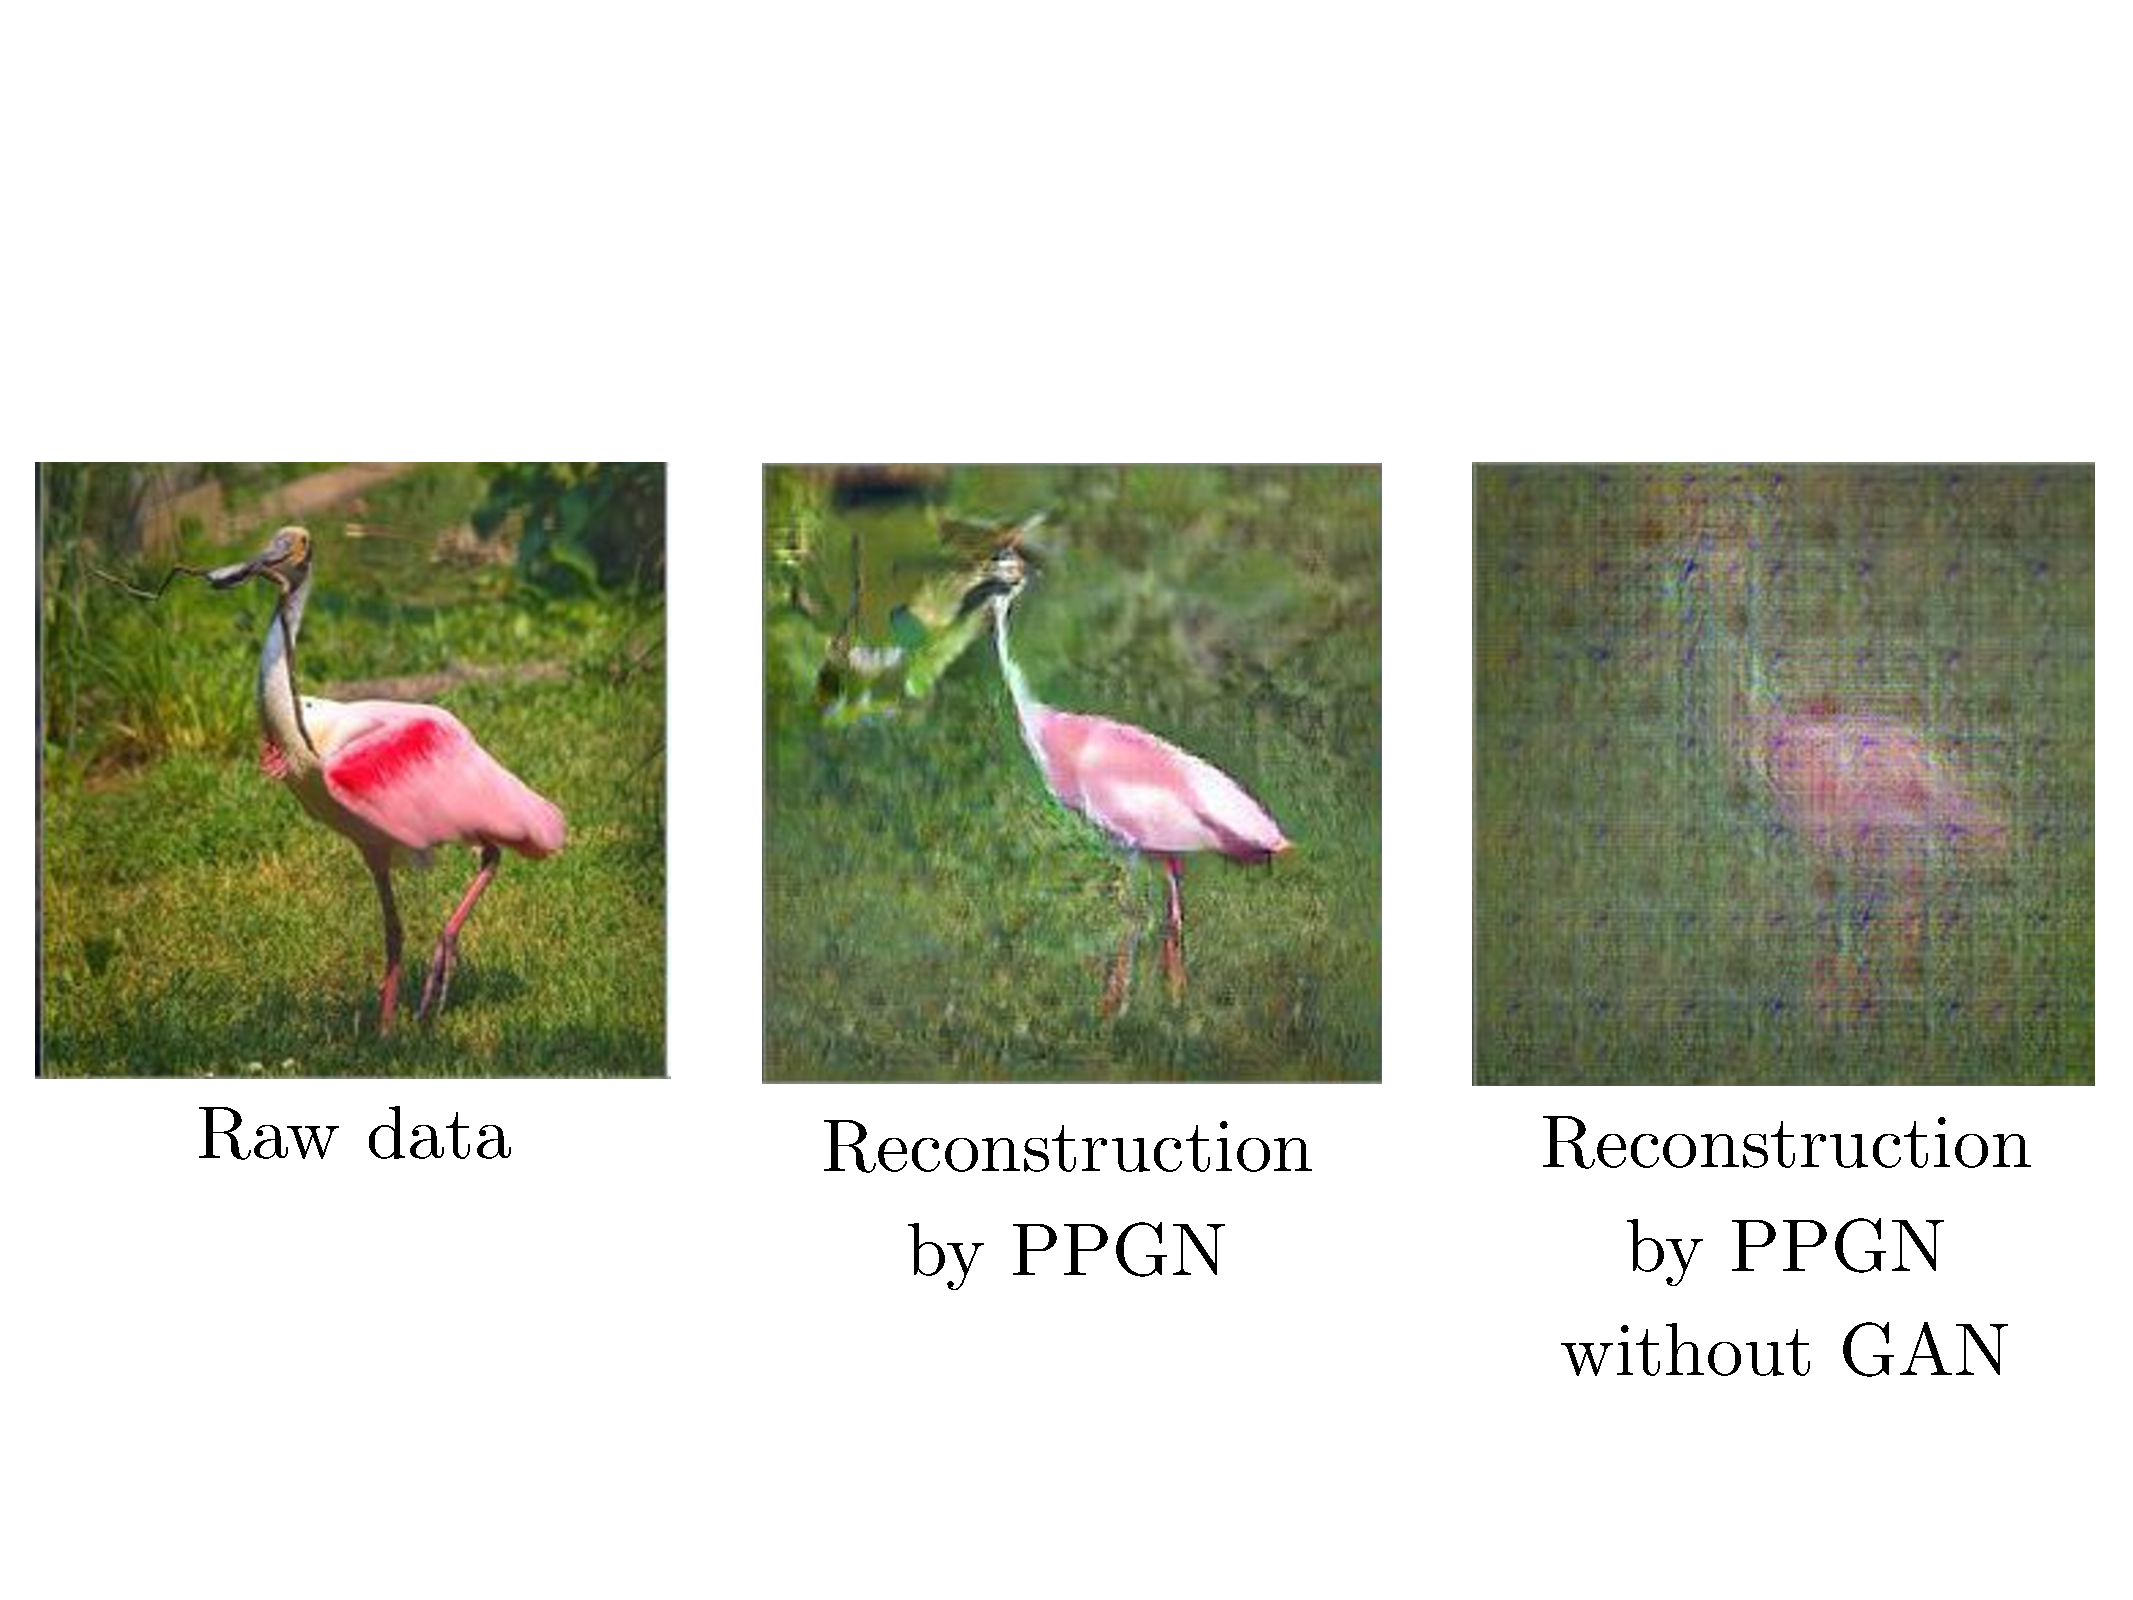
\includegraphics[width=\figwidth]{recons}
\caption{The GAN loss is a crucial ingredient of PPGNs. Without it, the denoising autoencoder
used to drive PPGNs does not create compelling images.}
\label{fig:recons}
\end{figure}



\section{Exercises}

This tutorial includes three exercises to check your understanding.
The solutions are given in \secref{sec:solutions}.

\subsection{The optimal discriminator strategy}
\label{sec:opt_d}

As described in \eqref{eq:discriminator_cost}, the goal of the discriminator is to minimize
\begin{equation}
  J^{(D)}(\vtheta^{(D)}, \vtheta^{(G)}) = -\frac{1}{2} \E_{\vx \sim \pdata} \log D(\vx) - \frac{1}{2} \E_{\vz} \log \left(1 - D\left( G(z) \right) \right)
\end{equation}
with respect to $\vtheta^{(D)}$.
Imagine that the discriminator can be optimized in function space, so the value of
$D(\vx)$ is specified independently for every value of $\vx$.
What is the optimal strategy for $D$?
What assumptions need to be made to obtain this result?

\subsection{Gradient descent for games}
\label{sec:xy_exercise}

Consider a minimax game with two players that each control a single scalar value.
The minimizing player controls scalar $x$ and the maximizing player controls
scalar $y$.
The value function for this game is
\[ V(x, y) = x y .\]

\begin{itemize}
  \item Does this game have an equilibrium? If so, where is it?
  \item Consider the learning dynamics of simultaneous gradient descent.
        To simplify the problem, treat gradient descent as a continuous time
        process.
        With an infinitesimal learning rate, gradient descent is described by a system of partial differential equations:
        \begin{align}
          \frac{\partial x}{\partial t} &= - \frac{\partial}{\partial x} V\left( x(t), y(t) \right) \\
          \frac{\partial y}{\partial t} &= \frac{\partial}{\partial y} V\left( x(t), y(t) \right).
        \end{align}
        Solve for the trajectory followed by these dynamics.
\end{itemize}



\subsection{Maximum likelihood in the GAN framework}
\label{sec:mle_exercise}
TODO

\section{Solutions to exercises}
\label{sec:solutions}

\subsection{The optimal discriminator strategy}
\label{sec:opt_d_soln}

Our goal is to minimize
\begin{equation}
  J^{(D)}(\vtheta^{(D)}, \vtheta^{(G)}) = -\frac{1}{2} \E_{\vx \sim \pdata} \log D(\vx) - \frac{1}{2} \E_{\vz} \log \left(1 - D\left( G(z) \right) \right)
\end{equation}
in function space, specifying $D(\vx)$ directly.

We begin by assuming that both $\pdata$ and $\pmodel$ are nonzero everywhere.
If we do not make this assumption, then some points are never visited during training,
and have undefined behavior.

To minimize $J^{(D)}$ with respect to $D$, we can write down the functional derivatives with
respect to a single entry $D(\vx)$, and set them equal to zero:
\[
\frac{\delta} {\delta D(\vx)} J^{(D)} = 0.
\]
By solving this equation, we obtain
\[
D^*(\vx) = \frac{ \pdata(\vx) } {\pdata(\vx) + \pmodel(\vx) }.
\]

Estimating this ratio is the key approximation mechanism used by GANs.

The process is illustrated in \figref{fig:ratio}.

\begin{figure}
\centering
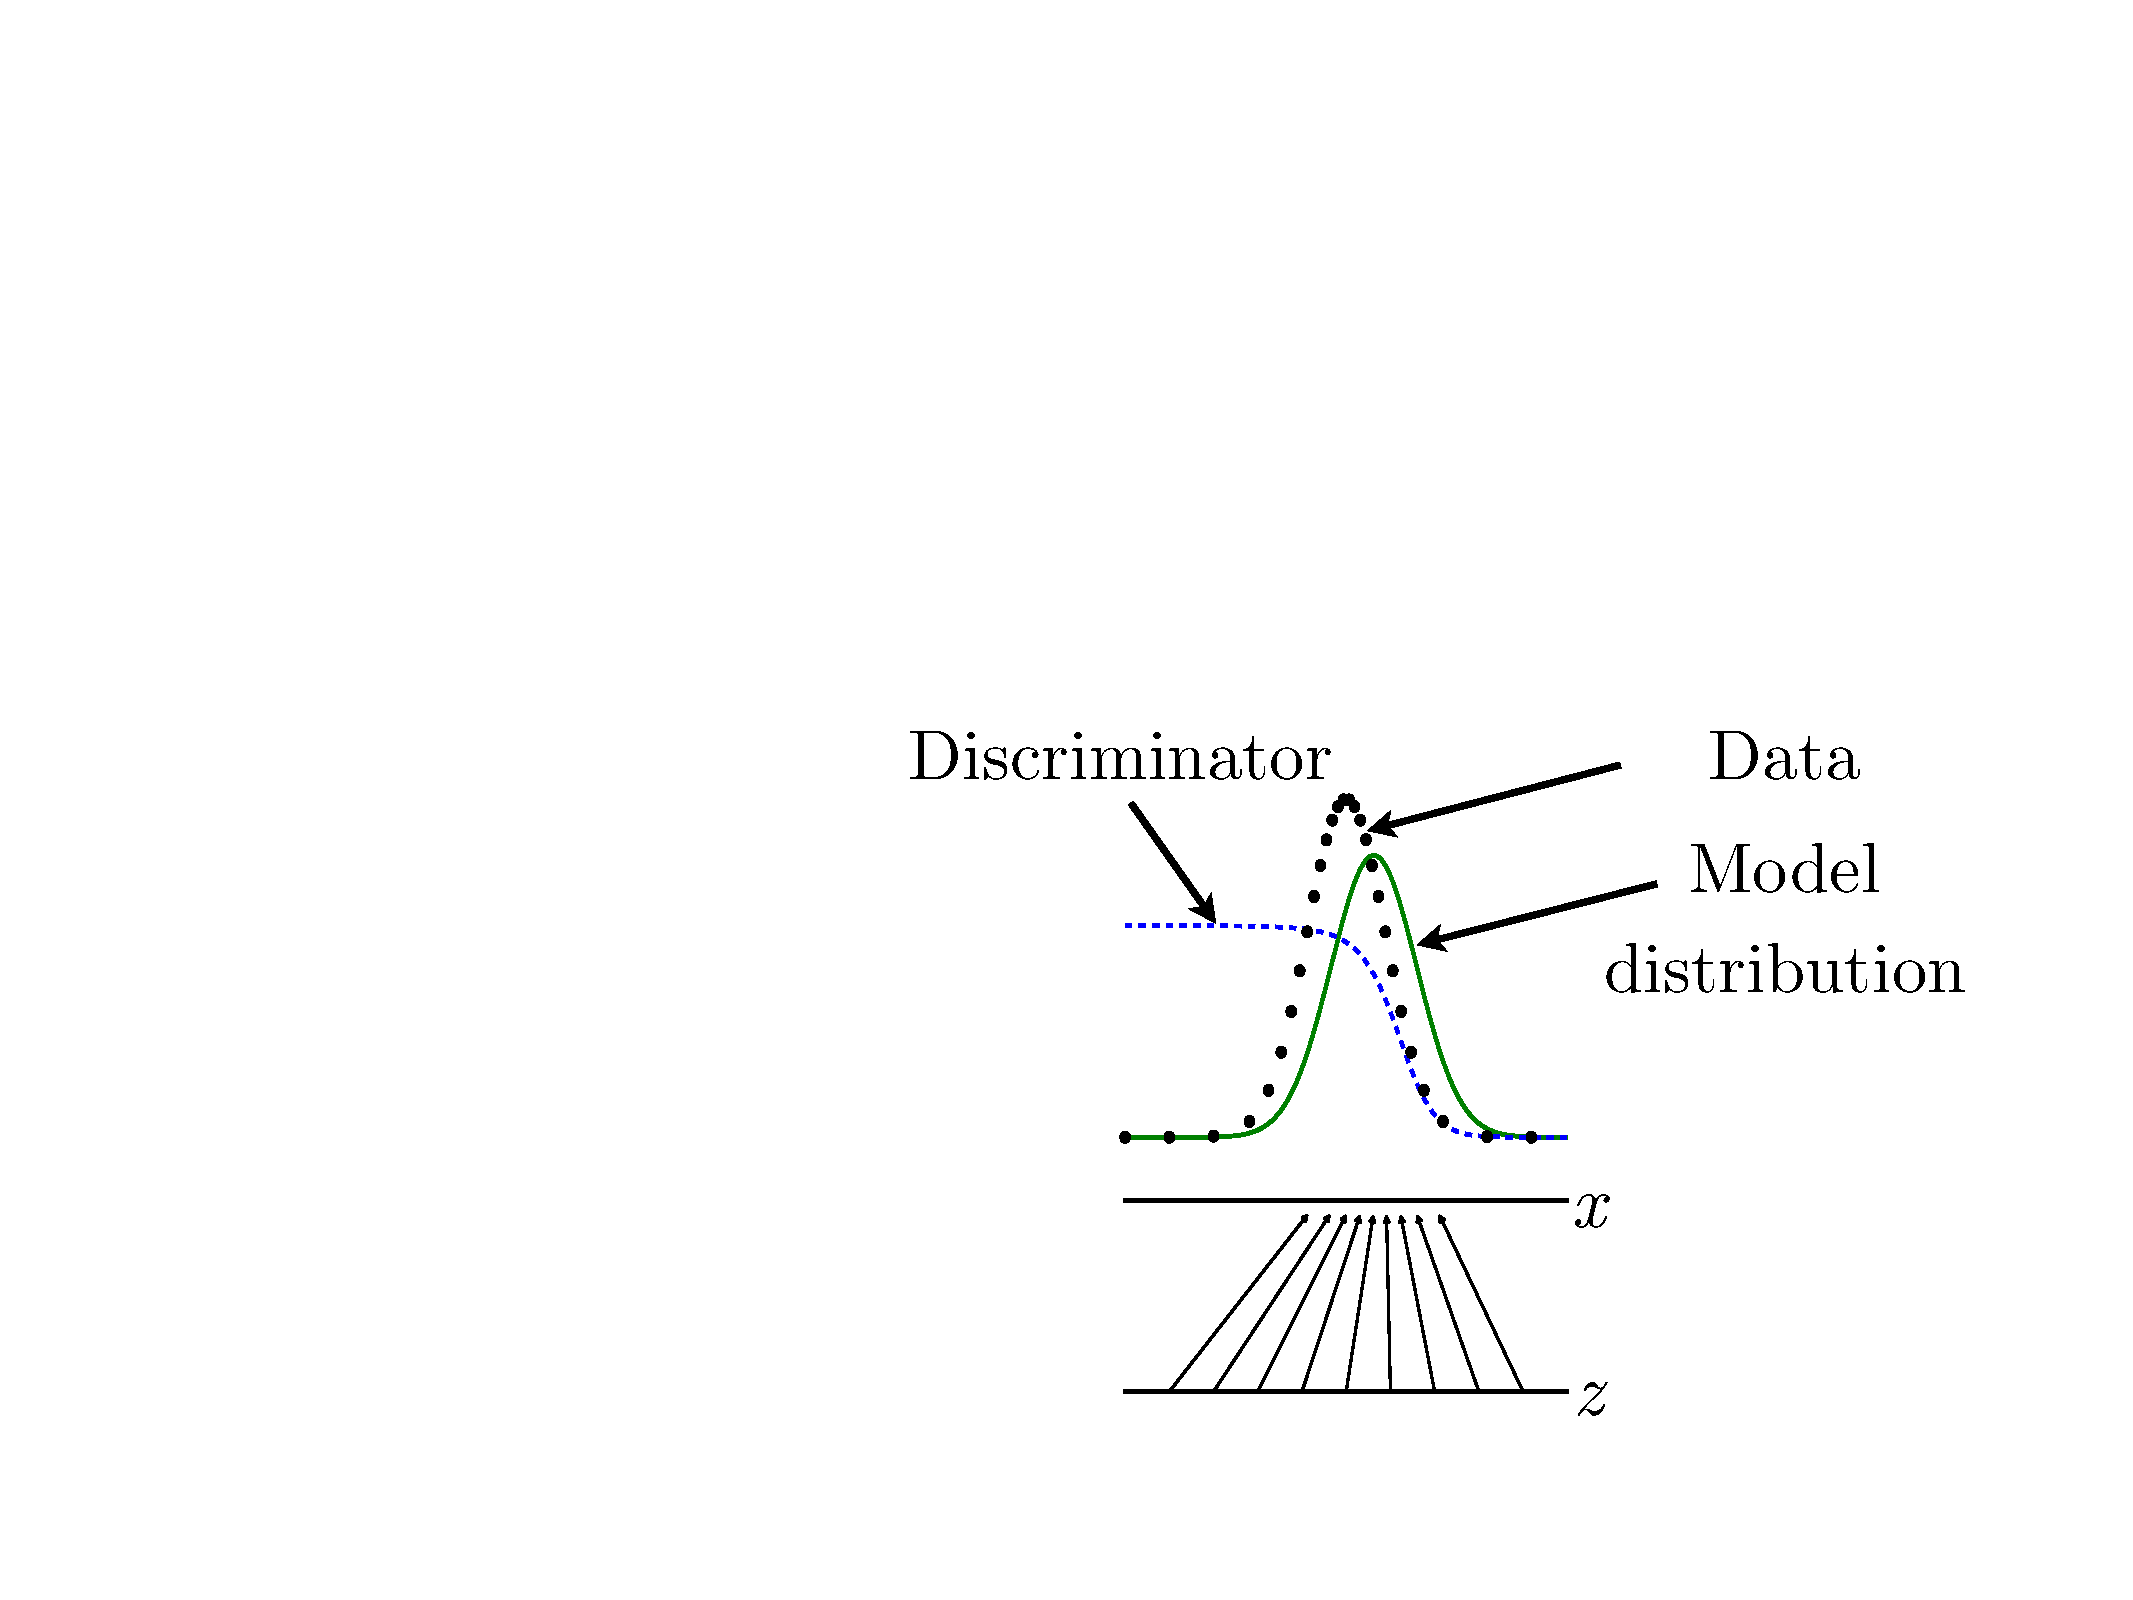
\includegraphics[width=\figwidth]{ratio}
\caption{
An illustration of how the discriminator estimates a ratio of
densities.
In this example, we assume that both $z$ and $x$ are one dimensional
for simplicity.
The mapping from $z$ to $x$ (shown by the black arrows) is non-uniform so that $\pmodel(x)$
(shown by the green curve) is
greater in places where $z$ values are brought together more densely.
The discriminator (dashed blue line) estimates the ratio between the data density (black dots)
and the sum of the data and model densities.
Wherever the output of the discriminator is large, the model density is too low, and wherever
the output of the discriminator is small, the model density is too high.
The generator can learn to produce a better model density by following the discriminator uphill;
each $G(z)$ value should move slightly in the direction that increases $D(G(z))$.
Figure reproduced from \citet{Goodfellow-et-al-NIPS2014-small}.
}
\label{fig:ratio}
\end{figure}


\subsection{Gradient descent for games}
\label{sec:xy_soln}

The value function
\[ V(x, y) = x y \]
is the simplest possible example of a continuous function with a saddle point.
It is easiest to understand this game by visualizing the value function in three
dimensions, as shown in \figref{fig:xy}.

\begin{figure}
\centering
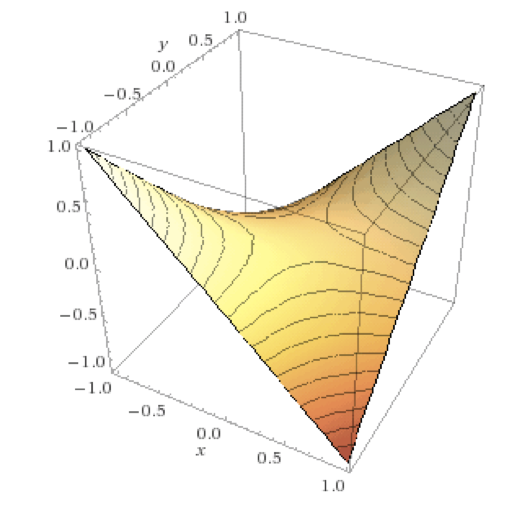
\includegraphics[width=\figwidth]{xy}
\caption{A three-dimensional visualization of the value function $V(x,y) = xy$.
  This is the canonical example of a function with a saddle point, at $x=y=0$.
}
\label{fig:xy}
\end{figure}

The three dimensional visualization shows us clearly that there is a saddle point
at $x=y=0$. This is an equilibrium of the game. We could also have found this point
by solving for where the derivatives are zero.

Not every saddle point is an equilibrium; we require that an infinitesimal perturbation
of one player's parameters cannot reduce that player's cost.
The saddle point for this game satisfies that requirement.
It is something of a pathological equilibrium because the value function is constant
as a function of each player's parameter when holding the other player's parameter
fixed.

To solve for the trajectory taken by gradient descent, we take the derivatives, and find that
\begin{align}
  \frac{\partial x}{\partial t} = - y(t) \\
  \frac{\partial y}{\partial t} = x(t). \label{eq:dy}
\end{align}
Diffentiating \eqref{eq:dy}, we obtain
\[
  \frac{\partial^2 y}{\partial t^2} = \frac{\partial x}{\partial t} = -y(t).
\]
Differential equations of this form have sinusoids as their set of basis functions
of solutions.
Solving for the coefficients that respect the boundary conditions, we obtain
\begin{align}
  x(t) = x(0) \cos(t) - y(0) \sin(t) \\
  y(t) = x(0) \sin(t) + y(0) \cos(t).
\end{align}

These dynamics form a circular orbit, as shown in \figref{fig:orbit}.
In other words, simultaneous gradient descent with an infinitesimal learning rate
will orbit the equilibrium forever, at the same radius that it was initialized.
With a larger learning rate, it is possible for simultaneous gradient descent to
spiral outward forever.
Simultaneous gradient descent will never approach the equilibrium.

\begin{figure}
  \center
  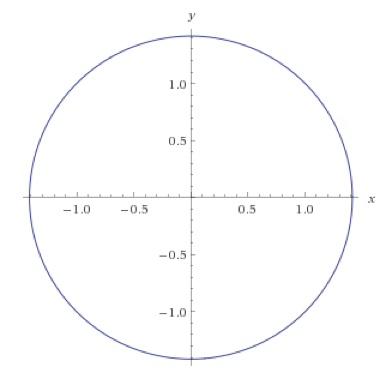
\includegraphics[width=\figwidth]{orbit}
  \caption{Simultaneous gradient descent with infinitesimal learning rate
    will orbit indefinitely at constant radius when applied to $V(x,y) = xy$,
    rather than approaching the equilibrium solution at $x=y=0$.
  }
  \label{fig:orbigt}
\end{figure}

For some games, simultaneous gradient descent does converge, and for others,
such as the one in this exercise, it does not.
For GANs, there is no theoretical prediction as to whether simultaneous
gradient descent should converge or not.
Settling this theoretical question, and developing algorithms guaranteed to
converge, remain important open research problems.

\subsection{Maximum likelihood in the GAN framework}
\label{sec:mle_soln}
TODO

\section{Conclusion}

GANs are generative models that use supervised learning to approximate an intractable cost
function, much as Boltzmann machines use Markov chains to approximate their cost and VAEs
use the variational lower bound to approximate their cost.
GANs can use this supervised ratio estimation technique to approximate many cost functions, including the KL divergence used for maximum
likelihood estimation.

GANs are relatively new and still require some research to reach their new potential.
In particular, training GANs requires finding Nash equilibria in high-dimensional,
continuous, non-convex games.
Researchers should strive to develop better theoretical understanding and better training
algorithms for this scenario.
Success on this front would improve many other applications, besides GANs.

GANs are crucial to many different state of the art image generation and manipulation systems,
and have the potential to enable many other applications in the future.

\section*{Acknowledgments}
The author would like to thank the NIPS organizers for inviting him to
present this tutorial.
Many thanks also to those who commented on his Twitter and Facebook posts
asking which topics would be of interest to the tutorial audience.
Thanks also to D. Kingma for helpful discussions regarding the description of VAEs.
Thanks to Zhu Xiaohu, Alex Kurakin and Ilya Edrenkin for spotting typographical errors in the
manuscript.

\bibliography{biblio}
\bibliographystyle{natbib}

\end{document}
